\documentclass{beamer}
%
% Choose how your presentation looks.
%
% For more themes, color themes and font themes, see:
% http://deic.uab.es/~iblanes/beamer_gallery/index_by_theme.html
%
\mode<presentation>
{
  \usetheme{Madrid}      % or try Darmstadt, Madrid, Warsaw, ...
  \usecolortheme{beaver} % or try albatross, beaver, crane, ...
  \usefonttheme{serif}  % or try serif, structurebold, ...
  \setbeamertemplate{navigation symbols}{}
  \setbeamertemplate{caption}[numbered]
  %%% Author/Title/Date and slide number in the footline
  \setbeamertemplate{footline}[author title date]
  %%% Puts the section/subsection in the headline
  \setbeamertemplate{headline}[section]
  
%%% Set a background colour
% \setbeamercolor{background canvas}{bg=lightgrey}
} 

\graphicspath{{./img/}}
\DeclareGraphicsExtensions{.pdf,.png,.jpg}

\usepackage[brazil]{babel}
%\usepackage[brazilian]{babel}
%\usepackage[T1]{fontenc} 
\usepackage{ae,url} 
\usepackage{amssymb,amsmath}
\usepackage[utf8]{inputenc}
\usepackage{comment} %% cc
\usepackage{listings}
\lstset{numbers=left, keepspaces=true, columns=flexible}

%%%% PARA OS TABLEAUX semanticos
\usepackage{tikz}
\usetikzlibrary{positioning}
\title[Your Short Title]{Tableaux Semânticos}
\tikzset{%
>=latex, %melhor aparência para as setas
inner sep=0pt,outer sep=0pt, %sem separação entre os nós
node distance=5mm %distância entre os nós
}
%%%% PARA OS TABLEAUX semanticos


\title{Lógica Matemática - LMA 0001}
\author{Rogério Eduardo da Silva - \textit{rogerio.silva@udesc.br}\\Claudio Cesar de Sá - \textit{claudio.sa@udesc.br}}
\institute{Universidade do Estado de Santa Catarina \\ Departamento de Ciência da Computação}
\date{\today}

% The log drawn in the upper right corner.
\logo{\includegraphics[height=0.03\paperheight]{udesc_joinville}}

\begin{document}
\bibliographystyle{apalike}

% DO NOT COMPILE THIS FILE DIRECTLY!
% This is included by the other .tex files.

\begin{frame}[t,plain]
\titlepage
\end{frame}

\begin{frame}
	Conteúdo Programático:
	\tableofcontents
\end{frame}

\section{Apresentação da Disciplina} % Necessário para gerar o \tableofcontents

\begin{frame}[t]{Método de Ensino} % Título do Frame
\begin{itemize}
	\item Aulas expositivas em sala e em laboratório
	\item Listas de exercícios teóricos e práticos
	\item Atendimento presencial (sala do professor) e/ou através da lista de emails da disciplina {\bf \url{lma-l@joinville.udesc.br}}
\end{itemize}
\end{frame}

\begin{frame}[t]{Avaliações} % Título do Frame
	\begin{itemize}
		\item 3 provas teóricas (30\% da média semestral cada uma)  \cite{edgar_2000, nunes_2002}: 
		   \begin{enumerate}
		   \item Conceitos básicos: tabelas-verdade, formas normais, implicação e equivalências lógica
		   \item Argumentação lógica: regras de inferência e de equivalência, demonstração condicional e por absurdo
	  	   \item Lógica de Primeira Ordem: Predicados, quantificadores, particularização/generalização
		   \end{enumerate}
		\item Projeto de Implementação Lógica em PROLOG (10\% da média semestral)
		\item Exame Final (caso média semestral < 7.0)\\ 
		Data prevista: {\bf 06 de Julho de 2015 -- 2a. Feira -- Sala F-101 -- 17:00 hrs}
	\end{itemize}
\end{frame}

\begin{frame}[t]{Bibliografia Básica Sugerida} % Título do Frame
    \bibliography{rogerio}
\end{frame}




% DO NOT COMPILE THIS FILE DIRECTLY!
% This is included by the other .tex files.

\section{Introdução à Lógica Proposicional} % Necessário para gerar o \tableofcontents

\begin{frame}[t]
\vskip 3cm
\begin{center}
{\Huge Introdução à\\Lógica Proposicional}
\end{center}
\end{frame}

\begin{frame}[t]
	\begin{figure}
		\center{\includegraphics[scale=0.9]{penguins.png}}
	\end{figure}
\end{frame}

\subsection{Definições Básicas}

\begin{frame}[t]{O que é Lógica?} % Título do Frame
\end{frame}

\begin{frame}[t]{O que é Lógica?} % Título do Frame
\begin{center}
``{\it Conhecimento das formas gerais e regras gerais do pensamento correto e verdadeiro, independentemente dos conteúdos pensados; regras para demonstração científica verdadeira; regras para pensamentos não-científicos; regras sobre o modo de expor o conhecimento; regras para verificação da verdade ou falsidade de um pensamento etc.}''
\end{center}

\begin{flushright}
\footnotesize{[Marilena Chaui, ``{\it Convite a Filosofia}'', 2002]}
\end{flushright}
\end{frame}

%\subsection{Conceitos Introdutórios}

\begin{frame}[t]{Conceitos Introdutórios} % Título do Frame
	\begin{itemize}
		\item Proposição
		   \begin{itemize}
		   \item conjunto de palavras ou símbolos que exprimem um pensamento (fatos ou juízos) de sentido completo
		   \item Exemplos
		   \begin{enumerate}
		   \item A Lua é o satélite da Terra
		   \item Recife é a capital de Pernambuco
	              \item $\pi > \sqrt{5}$
	 	   \item $1 + 1 = 3$
		   \end{enumerate}
		   \end{itemize}
		\item Princípios das Proposições
                         \begin{description}
		    \item[Não contradição:] uma proposição não pode ser verdadeira e falsa ao mesmo tempo
  		    \item[Terceiro excluído:] uma proposição é sempre ou verdadeira ou falsa, não existe terceira opção
		    \end{description}
	\end{itemize}
\end{frame}

\begin{frame}[t]{Conceitos Introdutórios} % Título do Frame
	\begin{itemize}
		\item Proposições {\bf Verdadeiras}
		   \begin{enumerate}
	 	   \item $1 + 1 = 2$
		   \item A Lua é o satélite natural da Terra
		   \item Florianópolis e Recife são capitais de estados
		   \end{enumerate}
		\item Proposições {\bf Falsas}
		   \begin{enumerate}
	 	   \item Vasco da Gama descobriu o Brasil
		   \item $3 \times 4 < 100 \div 13$
		   \item $3 \div 5$ é um número inteiro
		   \end{enumerate}
	\end{itemize}
\end{frame}

\begin{frame}[t]{Conceitos Introdutórios} % Título do Frame
	Determine ``V'' ou ``F'' para as afirmações abaixo
	\begin{enumerate}
	  \item O Brasil já ganhou 5 títulos mundiais
	\end{enumerate}
\end{frame}

\begin{frame}[t]{Conceitos Introdutórios} % Título do Frame
	Determine ``V'' ou ``F'' para as afirmações abaixo
	\begin{enumerate}
	  \item O Brasil já ganhou 5 títulos mundiais
	  \item $\pi = 3.14$
	\end{enumerate}
\end{frame}

\begin{frame}[t]{Conceitos Introdutórios} % Título do Frame
	Determine ``V'' ou ``F'' para as afirmações abaixo
	\begin{enumerate}
	  \item O Brasil já ganhou 5 títulos mundiais
	  \item $\pi = 3.14$
	  \item Eu sempre minto
	\end{enumerate}
\end{frame}

\begin{frame}[t]{Conceitos Introdutórios} % Título do Frame
	Determine ``V'' ou ``F'' para as afirmações abaixo
	\begin{enumerate}
	  \item O Brasil já ganhou 5 títulos mundiais
	  \item $\pi = 3.14$
	  \item Eu sempre minto
	\end{enumerate}
	
	\vskip 1cm

	\begin{center}
	{\Huge {\sc Cuidado com paradoxos!}}
	\end{center}
\end{frame}

\begin{frame}[t]{Conceitos Introdutórios} % Título do Frame
	Determine ``V'' ou ``F'' para as afirmações abaixo
	\begin{enumerate}
	  \item O Brasil já ganhou 5 títulos mundiais
	  \item $\pi = 3.14$
	  \item Eu sempre minto
	\end{enumerate}
	
	\vskip 1cm

	\begin{center}
	{\Huge {\sc Cuidado com paradoxos!}} 

	\vskip 1cm

	{\it I don't speak English}

	\end{center}
\end{frame}


\begin{frame}[t]{Função de Avaliação ou Interpretação Lógica} % Título do Frame
	
%\textcolor{red}{Rogério: introduzi este conceito nos
%exemplos anteriores.}\\


\begin{description}

\item[Uma proposição:]   uma proposição $p$ sempre assume $V$ ou $F$.  Nunca os
dois valores simultaneamente, ou nenhum dos dois. 
Sempre é alguma coisa em $V$ ou $F$, logo ...

  \item[Mapeamento Binário:]  $f(p) \to V$ ou  $f(p) \to F$
	
  \item[Função de Avaliação:] $f_{avalia}(p) = \{V, F\}$\\
%Fiz vários exercícios com os alunos sobre isto, interpretando
%proposições.

\item[Função de Avaliação $f(p)$ ou Interpretação Lógica $\Phi(p)$:] $f_{avalia}(p) \equiv \Phi(p)$

\item[Resumindo $f(p)$ ou $\Phi(p)$:] são utilizadas  para especificar o valor final sobre o conjunto
 $\{V, F\}$,   de uma fórmula lógica ou proposição composta



	\end{description}
\end{frame}




\begin{frame}[t]{Conceitos Introdutórios} % Título do Frame
	Alfabeto
	\begin{description}
	  \item[Símbolos Ortográficos:] ( )
	  \item[Constantes Lógicas:] {\em True, False} ({\bf V} e {\bf F} neste curso)
	  \item[Símbolos Proposicionais:] $p, q, r, s, p_1, r_2, \ldots$
	  \item[Conectores:] $\sim (\neg), \wedge, \vee, \rightarrow, \leftrightarrow$
	\end{description}
\end{frame}

\begin{frame}[t]{Conceitos Introdutórios} % Título do Frame
	Fórmulas bem formadas ({\em fbf})
	\begin{itemize}
	  \item Constantes lógicas são fórmulas
	  \item Símbolos proposicionais são fórmulas
	  \item Operação negação: $\sim p$
	  \item Operação conjunção (``e''): $p \wedge q$
	  \item Operação disjunção (``ou''): $p \vee q$
	  \item Operação disjunção exclusiva (``x-ou''): $p\veebar q$
	  \item Operação condicional: $p \rightarrow q$
	  \item Operação bicondicional:$p \leftrightarrow q$
	\end{itemize}
\end{frame}

\begin{frame}[t]{Conceitos Introdutórios} % Título do Frame
	Tabelas-Verdade
	\begin{itemize}
	  \item lista todos os possíveis valores lógicos de uma proposição composta, em função das combinações de todos os possíveis valores para cada proposição simples que a compõe
	  \item Exemplo:  $p \wedge q$
	    \begin{itemize}
	    \item Valores possíveis para ``p'' = V ou F (1 ou 0)
	    \item Valores possíveis para ``q'' = V ou F (1 ou 0)
	   \end{itemize}
	\end{itemize}

	\begin{minipage}[t]{0.45\textwidth}
	\begin{center}	
	\begin{tabular}{|c|c|}
	\hline
	$\mathbf{p}$ & $\mathbf{q}$ \\
	\hline
	V & V \\
	\hline
	V & F \\
	\hline
	F & V \\
	\hline
	F & F \\
	\hline
	\end{tabular}
	\end{center}
	\end{minipage}
	\begin{minipage}[t]{0.45\textwidth}
	\begin{center}	
	\begin{tabular}{|c|c|}
	\hline
	$\mathbf{p}$ & $\mathbf{q}$ \\
	\hline
	0 & 0 \\
	\hline
	0 & 1 \\
	\hline
	1 & 0 \\
	\hline
	1 & 1 \\
	\hline
	\end{tabular}
	\end{center}
	\end{minipage}
\end{frame}

\begin{frame}[t]{Conceitos Introdutórios} % Título do Frame
	Operações Lógicas: {\bf negação} ($\sim$)
	\begin{itemize}
	  \item inversão do valor lógico de uma proposição
	\end{itemize}

	\begin{center}	
	\begin{tabular}{|c|c|}
	\hline
	$\mathbf{p}$ & $\mathbf{\sim p}$ \\
	\hline
	V & F \\
	\hline
	F & V \\
	\hline
	\end{tabular}
	\end{center}
\end{frame}

\begin{frame}[t]{Conceitos Introdutórios} % Título do Frame
	Operações Lógicas: {\bf negação} ($\sim$)
	\begin{itemize}
	  \item Exemplos em Linguagem Natural:
	  \begin{itemize}
	  \item $p:$ O Sol é uma estrela
	  \item $\sim p:$ O Sol não é uma estrela
	  \item $p:$ Carlos é um mecânico
	  \item $\sim p:$ Não é verdade que Carlos é um mecânico
	  \item $\sim p:$ É falso que Carlos é um mecânico
	  \end{itemize}
	\end{itemize}
\end{frame}

\begin{frame}[t]{Conceitos Introdutórios} % Título do Frame
	Operações Lógicas: {\bf conjunção} ($\wedge$)
	\begin{itemize}
	  \item proposição composta que é verdadeira somente quando todas as proposições componentes forem verdadeiras
	\end{itemize}

	\begin{center}	
	\begin{tabular}{|c|c|c|}
	\hline
	$\mathbf{p}$ & $\mathbf{q}$ & $\mathbf{p \wedge q}$ \\
	\hline
	V & V & V \\
	\hline
	V & F & F \\
	\hline
	F & V & F \\
	\hline
	F & F & F \\
	\hline
	\end{tabular}
	\end{center}
\end{frame}

\begin{frame}[t]{Conceitos Introdutórios} % Título do Frame
	Operações Lógicas: {\bf disjunção} ($\vee$)
	\begin{itemize}
	  \item proposição composta que é verdadeira quando pelo menos uma das proposições componentes for verdadeira
	\end{itemize}

	\begin{center}	
	\begin{tabular}{|c|c|c|}
	\hline
	$\mathbf{p}$ & $\mathbf{q}$ & $\mathbf{p \vee q}$ \\
	\hline
	V & V & V \\
	\hline
	V & F & V \\
	\hline
	F & V & V \\
	\hline
	F & F & F \\
	\hline
	\end{tabular}
	\end{center}
\end{frame}

\begin{frame}[t]{Conceitos Introdutórios} % Título do Frame
	Operações Lógicas: {\bf disjunção exclusiva} ($\veebar$)
	\begin{itemize}
	  \item proposição composta que é verdadeira somente quando exatamente uma das proposições componentes for verdadeira
	\end{itemize}

	\begin{center}	
	\begin{tabular}{|c|c|c|}
	\hline
	$\mathbf{p}$ & $\mathbf{q}$ & $\mathbf{p \veebar q}$ \\
	\hline
	V & V & F \\
	\hline
	V & F & V \\
	\hline
	F & V & V \\
	\hline
	F & F & F \\
	\hline
	\end{tabular}
	\end{center}
\end{frame}

\begin{frame}[t]{Conceitos Introdutórios} % Título do Frame
	Operações Lógicas: {\bf condicional} ($\rightarrow$)
	\begin{itemize}
	  \item proposição que representa uma relação do tipo: ``{\bf se p então q}''
	  \item $p$ é chamado {\bf antecedente}
	  \item $q$ é chamado {\bf consequente}
	  \item $\rightarrow$ é chamado operador {\bf implicação}
	\end{itemize}

	\begin{center}	
	\begin{tabular}{|c|c|c|}
	\hline
	$\mathbf{p}$ & $\mathbf{q}$ & $\mathbf{p \rightarrow q}$ \\
	\hline
	V & V & V \\
	\hline
	V & F & F \\
	\hline
	F & V & V \\
	\hline
	F & F & V \\
	\hline
	\end{tabular}
	\end{center}
\end{frame}

\begin{frame}[t]{Conceitos Introdutórios} % Título do Frame
	Operações Lógicas: {\bf condicional} ($\rightarrow$)
	\begin{itemize}
	  \item Exemplos em Linguagem Natural:
	  \begin{itemize}
	  \item Se Maio tem 31 dias então a Terra é plana
	  \item Se $\pi$ é um número real então o Brasil fica na América do Sul
	  \end{itemize}
	\end{itemize}
\end{frame}

\begin{frame}[t]{Conceitos Introdutórios} % Título do Frame
	Operações Lógicas: {\bf bi-condicional} ($\leftrightarrow$)
	\begin{itemize}
	  \item proposição que representa uma relação do tipo: ``{\bf p se e somente se q}''
	\end{itemize}

	\begin{center}	
	\begin{tabular}{|c|c|c|}
	\hline
	$\mathbf{p}$ & $\mathbf{q}$ & $\mathbf{p \leftrightarrow q}$ \\
	\hline
	V & V & V \\
	\hline
	V & F & F \\
	\hline
	F & V & F \\
	\hline
	F & F & V \\
	\hline
	\end{tabular}
	\end{center}
\end{frame}

\begin{frame}[t]{Conceitos Introdutórios -- Exercícios} % Título do Frame
	Sejam as proposições 

	\begin{center}
	p: Está frio\\
	q: Está chovendo
	\end{center} 

	Traduzir para linguagem natural:

	\begin{enumerate}
	  \item $\sim p$
	  \item $p \wedge q$
	  \item $p \vee q$
	  \item $p \rightarrow \sim q$
	  \item $p \leftrightarrow q$
	  \item $\sim p \wedge \sim q$
	\end{enumerate}
\end{frame}

\begin{frame}[t]{Conceitos Introdutórios -- Exercícios} % Título do Frame
	Traduzir para linguagem simbólica:

	\begin{enumerate}
	  \item Marcos é alto e elegante
	  \item Marcos é alto mas não é elegante
	  \item Não é verdade que Marcos é baixo ou elegante
	  \item Marcos não é nem alto nem elegante
	  \item Marcos é alto ou é baixo e elegante
	\end{enumerate}
\end{frame}

\begin{frame}[t]{Conceitos Introdutórios -- Exercícios} % Título do Frame
	Determinar o valor lógico:

	\begin{enumerate}
	  \item Roma é a capital da França ou $tg 45^\circ = 1$
	  \item Não é verdade que 12 é impar
	  \item $2+2=4 \wedge$ 11 é primo
	  \item Se Brasília é a capital do Brasil então $\pi = 0$
	  \item Se Brasília é a capital do Brasil então argentinos falam espanhol
	  \item $3 + 2 = 7 ~\wedge~ 5 + 5 = 10 ~\vee~ 10 > 3 \times 3$
	  \item $\frac{10}{2} = 5  ~ \veebar ~  \sim 1 + 1 = 3$
	\end{enumerate}
\end{frame}

\subsection{Construção de Tabelas-Verdade}

\begin{frame}[t]
\vskip 2.5cm
\begin{center}
{\Huge Construção de\\Tabelas-Verdade}
\end{center}
\end{frame}

\begin{frame}[t]{Construção de Tabelas-Verdade} % Título do Frame
	\begin{itemize}
	  \item Número de Linhas = $2^N$, onde N = número de proposições
	  \item Dois Métodos:
	  \begin{enumerate}
	  \item uma coluna por operador 
             \item uma coluna por símbolo
	  \end{enumerate}
	\end{itemize}
\end{frame}

\begin{frame}[t]{Construção de Tabelas-Verdade} % Título do Frame
	Método \#1 - Uma coluna por operador.
	
	\begin{center}
	Exemplo: $\sim (p \wedge \sim q)$
	
	\vskip 0.8cm
		
	\begin{tabular}{|c|c|}
	\hline
	$\mathbf{p}$ & $\mathbf{q}$ \\
	\hline
	V & V \\
	\hline
	V & F \\
	\hline
	F & V \\
	\hline
	F & F \\
	\hline
	\end{tabular}
	\end{center}
\end{frame}

\begin{frame}[t]{Construção de Tabelas-Verdade} % Título do Frame
	Método \#1 - Uma coluna por operador.
	
	\begin{center}
	Exemplo: $\sim (p \wedge \sim q)$
	
	\vskip 0.8cm
		
	\begin{tabular}{|c|c|c|}
	\hline
	$\mathbf{p}$ & $\mathbf{q}$ & $\mathbf{\sim q}$\\
	\hline
	V & V & F\\
	\hline
	V & F & V \\
	\hline
	F & V & F \\
	\hline
	F & F & V \\
	\hline
	\end{tabular}
	\end{center}
\end{frame}

\begin{frame}[t]{Construção de Tabelas-Verdade} % Título do Frame
	Método \#1 - Uma coluna por operador.
	
	\begin{center}
	Exemplo: $\sim (p \wedge \sim q)$
	
	\vskip 0.8cm
		
	\begin{tabular}{|c|c|c|c|}
	\hline
	$\mathbf{p}$ & $\mathbf{q}$ & $\mathbf{\sim q}$ & $\mathbf{p \wedge \sim q}$ \\
	\hline
	V & V & F & F \\
	\hline
	V & F & V & V \\
	\hline
	F & V & F & F \\
	\hline
	F & F & V & F \\
	\hline
	\end{tabular}
	\end{center}
\end{frame}

\begin{frame}[t]{Construção de Tabelas-Verdade} % Título do Frame
	Método \#1 - Uma coluna por operador.
	
	\begin{center}
	Exemplo: $\sim (p \wedge \sim q)$
	
	\vskip 0.8cm
		
	\begin{tabular}{|c|c|c|c|c|}
	\hline
	$\mathbf{p}$ & $\mathbf{q}$ & $\mathbf{\sim q}$ & $\mathbf{p \wedge \sim q}$ & $\mathbf{\sim(p \wedge \sim q)}$ \\
	\hline
	V & V & F & F & V \\
	\hline
	V & F & V & V & F \\
	\hline
	F & V & F & F & V \\
	\hline
	F & F & V & F & V \\
	\hline
	\end{tabular}
	\end{center}
\end{frame}

\begin{frame}[t]{Construção de Tabelas-Verdade} % Título do Frame
	Método \#2 - Uma coluna por símbolo.
	
	\begin{center}
	Exemplo: $\sim (p \wedge \sim q)$
	
	\vskip 0.8cm
		
	\begin{tabular}{|c|c|c|c|c|}
	\hline
	& {\tiny 1} & & & {\tiny 1} \\
	\hline
	\hline
	$\mathbf{\sim}$ & $\mathbf{p}$ & $\mathbf{\wedge}$ & $\mathbf{\sim}$ & $\mathbf{q}$ \\
	\hline
	  & V &   &   & V \\
	\hline
	  & V &   &   & F \\
	\hline
	  & F &   &   & V \\
	\hline
	  & F &   &   & F \\
	\hline
	\end{tabular}
	\end{center}
\end{frame}

\begin{frame}[t]{Construção de Tabelas-Verdade} % Título do Frame
	Método \#2 - Uma coluna por símbolo.
	
	\begin{center}
	Exemplo: $\sim (p \wedge \sim q)$
	
	\vskip 0.8cm
		
	\begin{tabular}{|c|c|c|c|c|}
	\hline
	& {\tiny 1} & & {\tiny 2} & {\tiny 1} \\
	\hline
	\hline
	$\mathbf{\sim}$ & $\mathbf{p}$ & $\mathbf{\wedge}$ & $\mathbf{\sim}$ & $\mathbf{q}$ \\
	\hline
	  & V &   & F & V \\
	\hline
	  & V &   & V & F \\
	\hline
	  & F &   & F & V \\
	\hline
	  & F &   & V & F \\
	\hline
	\end{tabular}
	\end{center}
\end{frame}

\begin{frame}[t]{Construção de Tabelas-Verdade} % Título do Frame
	Método \#2 - Uma coluna por símbolo.
	
	\begin{center}
	Exemplo: $\sim (p \wedge \sim q)$
	
	\vskip 0.8cm
		
	\begin{tabular}{|c|c|c|c|c|}
	\hline
	& {\tiny 1} & {\tiny 3} & {\tiny 2} & {\tiny 1} \\
	\hline
	\hline
	$\mathbf{\sim}$ & $\mathbf{p}$ & $\mathbf{\wedge}$ & $\mathbf{\sim}$ & $\mathbf{q}$ \\
	\hline
	  & V & F & F & V \\
	\hline
	  & V & V & V & F \\
	\hline
	  & F & F & F & V \\
	\hline
	  & F & F & V & F \\
	\hline
	\end{tabular}
	\end{center}
\end{frame}

\begin{frame}[t]{Construção de Tabelas-Verdade} % Título do Frame
	Método \#2 - Uma coluna por símbolo.
	
	\begin{center}
	Exemplo: $\sim (p \wedge \sim q)$
	
	\vskip 0.8cm
		
	\begin{tabular}{|c|c|c|c|c|}
	\hline
	{\tiny 4} & {\tiny 1} & {\tiny 3} & {\tiny 2} & {\tiny 1} \\
	\hline
	\hline
	$\mathbf{\sim}$ & $\mathbf{p}$ & $\mathbf{\wedge}$ & $\mathbf{\sim}$ & $\mathbf{q}$ \\
	\hline
	V & V & F & F & V \\
	\hline
	F & V & V & V & F \\
	\hline
	V & F & F & F & V \\
	\hline
	V & F & F & V & F \\
	\hline
	\end{tabular}
	\end{center}
\end{frame}

\begin{frame}[t]{Construção de Tabelas-Verdade} % Título do Frame
	Concluindo:
	
	\begin{center}Exemplo: $\sim (p \wedge \sim q)$\end{center}

	$$P_{pq}(VV, VF, FV, FF) = (V, F, V, V)$$

	\begin{center}ou\end{center}

	$$P_{pq}(00, 01, 10, 11) = (1, 1, 0, 1)$$
\end{frame}

\begin{frame}[t]{Construção de Tabelas-Verdade - Exercícios} % Título do Frame
	\begin{enumerate}
	\item $\sim (p \wedge q) \vee\sim (q \leftrightarrow p)$
	\item $p \vee\sim r \rightarrow q \wedge\sim r$
	\item $(p \rightarrow q) \wedge (q \rightarrow r) \rightarrow (p \rightarrow r)$
	\end{enumerate}
\end{frame}

\begin{frame}[t]{Construção de Tabelas-Verdade - Exercícios} % Título do Frame
	\begin{enumerate}
	\item $\sim (p \wedge q) \vee\sim (q \leftrightarrow p)$
	   \begin{itemize} \item $P_{pq}(VV, VF, FV, VV) = (F, V, V, V)$ \end{itemize}
	\item $p \vee\sim r \rightarrow q \wedge\sim r$
	\item $(p \rightarrow q) \wedge (q \rightarrow r) \rightarrow (p \rightarrow r)$
	\end{enumerate}
\end{frame}

\begin{frame}[t]{Construção de Tabelas-Verdade - Exercícios} % Título do Frame
	\begin{enumerate}
	\item $\sim (p \wedge q) \vee\sim (q \leftrightarrow p)$
	   \begin{itemize} \item $P_{pq}(VV, VF, FV, VV) = (F, V, V, V)$ \end{itemize}
	\item $p \vee\sim r \rightarrow q \wedge\sim r$
	   \begin{itemize} \item $P_{pqr}(VVV, VVF, VFV, VFF, FVV, FVF, FFV, FFF) = (F, V, F, F, V, V, V, F)$ \end{itemize}
	\item $(p \rightarrow q) \wedge (q \rightarrow r) \rightarrow (p \rightarrow r)$
	\end{enumerate}
\end{frame}

\begin{frame}[t]{Construção de Tabelas-Verdade - Exercícios} % Título do Frame
	\begin{enumerate}
	\item $\sim (p \wedge q) \vee\sim (q \leftrightarrow p)$
	   \begin{itemize} \item $P_{pq}(VV, VF, FV, VV) = (F, V, V, V)$ \end{itemize}
	\item $p \vee\sim r \rightarrow q \wedge\sim r$
	   \begin{itemize} \item $P_{pqr}(VVV, VVF, VFV, VFF, FVV, FVF, FFV, FFF) = (F, V, F, F, V, V, V, F)$ \end{itemize}
	\item $(p \rightarrow q) \wedge (q \rightarrow r) \rightarrow (p \rightarrow r)$
	   \begin{itemize} \item $P_{pqr}(VVV, VVF, VFV, VFF, FVV, FVF, FFV, FFF) = (V, V, V, V, V, V, V, V)$ \end{itemize}
	\end{enumerate}
\end{frame}

% ============================================================================

%\subsection{Valor Lógico de uma Proposição}

\begin{frame}[t]{Valor Lógico de uma Proposição} % Título do Frame
	\begin{itemize}
	\item É obtido a partir da substituição das proposições componentes por seus respectivos valores lógicos.
	\item Exemplo:  

	\begin{center}p: A Terra é um planeta\\ q: Maio tem 30 dias\end{center}
	qual o valor lógico da proposição:

	\begin{itemize} \item $\sim (p \vee q) \leftrightarrow \sim p \wedge \sim q$ \end{itemize}
	\end{itemize}
\end{frame}

\begin{frame}[t]{Valor Lógico de uma Proposição} % Título do Frame
	\begin{itemize}
	\item É obtido a partir da substituição das proposições componentes por seus respectivos valores lógicos.
	\item Exemplo:  

	\begin{center}p: A Terra é um planeta\\ q: Maio tem 30 dias\end{center}
	qual o valor lógico da proposição:

	\begin{itemize} \item $\sim (p \vee q) \leftrightarrow \sim p \wedge \sim q$ \end{itemize}
	\end{itemize}
	
	\vskip 1cm

	\begin{center}
	$\sim (V \vee F) \leftrightarrow \sim V \wedge \sim F$ \\
	$\sim ( V ) \leftrightarrow F \wedge V$ \\
	$F \leftrightarrow F$ \\
	$V$
	\end{center}
\end{frame}

\begin{frame}[t]{Valor Lógico de uma Proposição - Exercícios} % Título do Frame
	\begin{enumerate}
	\item Para p = {\em falso} e q = {\em falso}, determine $(p \rightarrow q) \rightarrow (p \rightarrow p \wedge q)$
	\item Para p = {\em verdade} e q, r = {\em falso}, determine $(q \leftrightarrow (r \rightarrow \sim p)) \vee ((\sim q \rightarrow p) \leftrightarrow r)$
	\item Para r = {\em verdade}, determine: $p \rightarrow \sim q \vee r$
	\item Para q = {\em verdade}, determine: $(p \rightarrow q) \rightarrow (\sim q \rightarrow \sim p)$
	\end{enumerate}
\end{frame}

\begin{frame}[t]{Uso de Parênteses} % Título do Frame
	\begin{itemize}
	\item A expressão $p \wedge q \vee r$ pode ser interpretada de duas formas (com valores lógicos distintos):
	\begin{enumerate}
	\item $(p \wedge q) \vee r$
	\item $p \wedge (q \vee r)$
	\end{enumerate}

	\begin{figure}
		\center{\includegraphics[scale=0.7]{usoparent.png}}
	\end{figure}
	\end{itemize}
\end{frame}

\begin{frame}[t]{Uso de Parênteses} % Título do Frame
	\begin{itemize}
	\item Ordem de Precedência dos conectivos:
	\begin{enumerate}
	\item $\sim$
	\item $\wedge ~ \vee ~ \veebar$
	\item $\rightarrow$
	\item $\leftrightarrow$
	\end{enumerate}

	\item {\sc Exercício:} Monte a representação hierárquica para as expressões abaixo:
	\begin{enumerate}
	\item $p \wedge \sim q$
	\item $p \wedge q \veebar r$
	\item $\sim (p \rightarrow q \vee \sim r)$
	\item $p \wedge q \rightarrow \sim p$
	\item $p \wedge (q \rightarrow \sim p)$
	\item $q \rightarrow p \leftrightarrow r \wedge s \vee \sim t$
	\end{enumerate}
	\end{itemize}
\end{frame}

\begin{frame}[t]{Uso de Parênteses} % Título do Frame
	\begin{itemize}
	\item Ordem de Precedência dos conectivos:
	\begin{enumerate}
	\item $\sim$
	\item $\wedge ~ \vee ~ \veebar$
	\item $\rightarrow$
	\item $\leftrightarrow$
	\item $( \ldots )$
	\end{enumerate}

	\item os símbolos de parênteses ``( )'' são então utilizados como modificadores da ordem de precedência.
	\end{itemize}
\end{frame}

\begin{frame}[t]{Construção de Tabelas-Verdade - Exercícios} % Título do Frame
	\begin{enumerate}
	\item $\sim (p \vee \sim q)$
	\item $\sim (p \rightarrow \sim q)$
	\item $p \wedge q \rightarrow p \vee q$
	\item $\sim p \rightarrow (q \rightarrow p)$
	\item $(p \rightarrow q) \rightarrow p \wedge q$
	\item $q \leftrightarrow \sim q \wedge p$
	\item $(p \leftrightarrow \sim q) \rightarrow \sim p \wedge q$
	\end{enumerate}
\end{frame}

\begin{frame}[t]{Construção de Tabelas-Verdade - Exercícios} % Título do Frame
	Suprimir o maior número de parênteses possível (de forma a não alterar a expressão):
	\begin{enumerate}
	\item $((q \leftrightarrow (r \vee q)) \leftrightarrow (p \wedge (\sim (\sim q))))$
	\item $((p \wedge (\sim (\sim q))) \leftrightarrow (q \leftrightarrow (r \vee q)))$
	\item $(((p \vee q) \rightarrow (\sim r)) \vee ((((\sim q) \wedge r) \wedge q)))$
	\end{enumerate}
\end{frame}

% ============================================================================

%\subsection{Tautologias, Contradições e Contingências}

\begin{frame}[t]{Tautologias, Contradições e Contingências} % Título do Frame
	Tautologia ($\blacksquare$):
	\begin{itemize}
	\item Toda proposição $P_{pqr\ldots}$ que, \underline{independente} dos valores lógicos de suas proposições componentes, resulte sempre em {\bf verdade}.
	\item Exemplo: \begin{center}$\sim (p \wedge \sim p)$ \end{center}

	\vskip 1cm
	
	\begin{center}
	\begin{tabular}{|c|c|c|c|}
	\hline
	$\mathbf{p}$ & $\mathbf{\sim p}$ & $\mathbf{p \wedge \sim p}$ & $\mathbf{\sim(p \wedge\sim p)}$ \\
	\hline
	V & F & F & V \\
	\hline
	F & V & F & V \\
	\hline
	\end{tabular}
	\end{center}

	$$P_p(V, F) = (V, V) = \blacksquare$$
	\end{itemize}
\end{frame}

\begin{frame}[t]{Tautologias, Contradições e Contingências} % Título do Frame
	Outros exemplos:
	\begin{itemize}
	\item $p \vee\sim p$
	\item $p \vee\sim (p \wedge q)$
	\item $p \wedge q \rightarrow (p \leftrightarrow q)$
	\item $p \vee (q \wedge\sim q) \leftrightarrow p$
	\item $p \vee r \rightarrow \sim q \vee r$
	\item $((p \rightarrow q) \rightarrow r) \rightarrow (p \rightarrow (q \rightarrow r))$
	\end{itemize}
\end{frame}

\begin{frame}[t]{Tautologias, Contradições e Contingências} % Título do Frame
	Tautologia ($\blacksquare$):\\
	\begin{center}Princípio da Substituição\end{center}
	\begin{itemize}
	\item Se $P_{pqr\ldots}$ é uma tautologia então $P_{p_0q_0r_0\ldots}$ também será uma tautologia, independente dos valores de $p_0, q_0, r_0, \ldots$ 
	\end{itemize}
\end{frame}

\begin{frame}[t]{Tautologias, Contradições e Contingências} % Título do Frame
	Contradição ($\square$):
	\begin{itemize}
	\item Toda proposição $P_{pqr\ldots}$ que, \underline{independente} dos valores lógicos de suas proposições componentes, resulte sempre em {\bf falsidade}.
	\item Exemplo: \begin{center}$p \wedge \sim p$ \end{center}

	\vskip 1cm

	\begin{center}
	\begin{tabular}{|c|c|c|}
	\hline
	$\mathbf{p}$ & $\mathbf{\sim p}$ & $\mathbf{p \wedge \sim p}$ \\
	\hline
	V & F & F \\
	\hline
	F & V & F \\
	\hline
	\end{tabular}
	\end{center}
	
	$$P_p(V, F) = (F, F) = \square$$
	\end{itemize}
\end{frame}

\begin{frame}[t]{Tautologias, Contradições e Contingências} % Título do Frame
	Outros exemplos:
	\begin{itemize}
	\item $p \leftrightarrow\sim p$
	\item $(p \wedge q) \wedge \sim (p \vee q)$
	\item $\sim p \wedge (p \wedge \sim q)$
	\end{itemize}
\end{frame}

\begin{frame}[t]{Tautologias, Contradições e Contingências} % Título do Frame
	Consistência (ou Contingência -- livro texto):
	\begin{itemize}
	\item Toda proposição $P_{pqr\ldots}$ que não é nem uma tautologia nem uma contradição.
	\item Isto é: pelo menos um $V$ e um $F$ em suas interpretações
	\item Exemplo: \begin{center}$p \rightarrow \sim p$ \end{center}

	\vskip 1cm
	
	\begin{center}
	\begin{tabular}{|c|c|c|}
	\hline
	$\mathbf{p}$ & $\mathbf{\sim p}$ & $\mathbf{p \rightarrow \sim p}$ \\
	\hline
	V & F & F \\
	\hline
	F & V & V \\
	\hline
	\end{tabular}
	\end{center}
	$$P_p(V, F) = (F, V)$$
	\end{itemize}
\end{frame}

\begin{frame}[t]{Tautologias, Contradições e Contingências - Exercícios} % Título do Frame
	Classifique as proposições abaixo como tautológicas, contraditórias (ou insatisfatível ou inconsistente) ou consistentes (ou satisfatível ou contingente):
	\begin{enumerate}
	\item $(p \rightarrow p) \vee (p \rightarrow\sim p)$
	\item $p \rightarrow (p \rightarrow q \wedge\sim q)$
	\item $(p \rightarrow q) \rightarrow (p \vee r \rightarrow q \vee r)$
	\end{enumerate}
\end{frame}
%%%%%%%%%%%%%%%%%%%%%%%%%%%%%%%%%%%%%%%%%%%%%%%%%%%%%%%%%%%%%%%%%
\begin{frame}[t]{Resumindo a nomenclatura dos tipos de fórmulas} % Título do Frame

\begin{block} {}
	\begin{itemize}
	\item Tautológica: sempre verdade ($\blacksquare $)
	\item Contraditórias ou insatisfatíveis ou inconsistentes ($\square$)
	\item Consistentes ou satisfatíveis ou contingentes (pelo menos um $V$ e um $F$ na TV)
	\end{itemize}
\end{block}	
\end{frame}
%%%%%%%%%%%%%%%%%%%%%%%%%%%%%%%%%%%%%%%%%%%%%%%%%%%%%%%%


% ============================================================================

\subsection{Implicação Lógica}

\begin{frame}[t]
\vskip 3.5cm
\begin{center}
{\Huge Implicação Lógica}
\end{center}
\end{frame}

\begin{frame}[t]%%%[allowframebreaks=0.9]

\frametitle{Implicação Lógica} % Título do Frame

\begin{block}{Definições:}
		\begin{itemize}
		
	\item Diz-se que uma fórmula $P_{pqr\ldots}$ {\em implica logicamente} uma outra fórmula $Q_{pqr\ldots}$, se simultaneamente estas 
	 nunca assumirem os valores lógicos ``V'' e ``F'', respectivamente, em suas tabelas verdades.
	 
	 \item Isto é uma definição: quando a fórmula  $P_{pqr\ldots}$ assumir $V$,
	 $Q_{pqr\ldots}$ nunca poderá ser $F$

	\item Representação: $$P_{pqr\ldots} \Rightarrow Q_{pqr\ldots}$$

	\item Toda fórmula (ora fórmula atômica ou proposição)  implica logicamente em 
	      uma tautologia: $P_{pqr\ldots} \Rightarrow\blacksquare$

	\item Só uma contradição implica logicamente em outra contradição: $\square \Rightarrow \square$
	
		
	\end{itemize}

	\end{block}
\end{frame}



\begin{frame}[t]%%%[allowframebreaks=0.9]

\frametitle{Implicação Lógica} % Título do Frame

\begin{block}{Definições:}
		\begin{itemize}
		
	
	\item \underline{Atenção}: o símbolo ``$\Rightarrow $'' define uma \textbf{relação lógica}    entre duas 
	fórmulas $P_{pqr\ldots}$ e $Q_{pqr\ldots}$

	\item Por outro lado,  o símbolo ``$\rightarrow $'' define uma \textbf{conectivo lógico} entre duas 
		fórmulas $P_{pqr\ldots}$ e $Q_{pqr\ldots}$. Aqui tem tabela-verdade, no caso acima não
		
		
	\item Em resumo: o ``$\Rightarrow $'' é uma  \textbf{relação	matemática}, enquanto o
	 ``$\rightarrow $'' é  um
	  \textbf{conectivo lógico} usado para construir fórmulas
	
	\end{itemize}

	\end{block}
\end{frame}

%--------------------------------------------------------------------




\begin{frame}[t]{Implicação Lógica} % Título do Frame



\begin{block}{Sua definição operacional é dada por:}

\begin{itemize}
\item Para verificar se duas fórmulas se relacionam logicamente entre si, isto é, $P_{pqr\ldots} \Rightarrow Q_{pqr\ldots}$, deve-se contruir as tabelas-verdade de $P_{pqr\ldots}$  e $Q_{pqr\ldots}$

\item Em toda linha de  avaliação de $P_{pqr\ldots}$ for \textbf{Verdade}, então naquela linha em $Q_{pqr\ldots}$ também deverá ser \textbf{Verdade}

\item Em outras palavras, a definição da relação de implicação lógica ($\Rightarrow$), segue a tabela-verdade da operação ou conectivo lógico da implicação ($\rightarrow$)
\end{itemize}
\end{block}
\end{frame}

%--------------------------------------------------------------------------------------------------


\begin{frame}[t]{Implicação Lógica} % Título do Frame
	Propriedades:
	\begin{itemize}
	\item Propriedade Reflexiva: $P_{pqr\ldots} \Rightarrow P_{pqr\ldots}$

	\item Propriedade Transitiva: se $P_{pqr\ldots} \Rightarrow Q_{pqr\ldots}$ e $Q_{pqr\ldots} \Rightarrow R_{pqr\ldots}$ então $P_{pqr\ldots} \Rightarrow R_{pqr\ldots}$

	\item Exemplo 01: para $p \wedge q, p \vee q ~e~ p \leftrightarrow q$:
	\begin{itemize}
	\item $p \wedge q \Rightarrow p \vee q$
	\item $p \wedge q \Rightarrow p \leftrightarrow q$
	\end{itemize}

	\item Exemplo 02: para $p \leftrightarrow q, p \rightarrow q ~e~ q \rightarrow p$:
	\begin{itemize}
	\item $p \leftrightarrow q \Rightarrow p \rightarrow q$
	\item $p \leftrightarrow q \Rightarrow q \rightarrow p$
	\end{itemize}
	
	\item Falta validar todos estes exemplos!
	\end{itemize}
\end{frame}





\begin{frame}[t]{Implicação Lógica} % Título do Frame

\frametitle{Regras de Inferência}

Construindo TVs, construa e valide as Implicações Lógicas que se seguem:

	\begin{description}
	\item[Adição:] 
		$\begin{array}{l}
		   p \Rightarrow p \vee q \\ 
		   q \Rightarrow p \vee q \\
		\end{array}$
	\end{description}
\end{frame}

\begin{frame}[t]{Implicação Lógica} % Título do Frame
	Regras de Inferência:
	\begin{description}
	\item[Adição:] 
		$\begin{array}{l}
		   p \Rightarrow p \vee q \\ 
		   q \Rightarrow p \vee q \\
		\end{array}$

	\item[Simplificação:] 
		$\begin{array}{l}
		  p \wedge q \Rightarrow p \\
		  p \wedge q \Rightarrow q \\
		\end{array}$
	\end{description}
\end{frame}

\begin{frame}[t]{Implicação Lógica} % Título do Frame
	Regras de Inferência:
	\begin{description}
	\item[Adição:] 
		$\begin{array}{l}
		   p \Rightarrow p \vee q \\ 
		   q \Rightarrow p \vee q \\
		\end{array}$

	\item[Simplificação:] 
		$\begin{array}{l}
		  p \wedge q \Rightarrow p \\
		  p \wedge q \Rightarrow q \\
		\end{array}$

	\item[Silogismo Disjuntivo:] 
		$\begin{array}{l}
		  (p \vee q) \wedge \sim p \Rightarrow q \\
		  (p \vee q) \wedge \sim q \Rightarrow p \\
		\end{array}$

	\end{description}
\end{frame}

\begin{frame}[t]{Implicação Lógica} % Título do Frame
	Regras de Inferência:
	\begin{description}
	\item[Adição:] 
		$\begin{array}{l}
		   p \Rightarrow p \vee q \\ 
		   q \Rightarrow p \vee q \\
		\end{array}$

	\item[Simplificação:] 
		$\begin{array}{l}
		  p \wedge q \Rightarrow p \\
		  p \wedge q \Rightarrow q \\
		\end{array}$

	\item[Silogismo Disjuntivo:] 
		$\begin{array}{l}
		  (p \vee q) \wedge \sim p \Rightarrow q \\
		  (p \vee q) \wedge \sim q \Rightarrow p \\
		\end{array}$

	\item[Modus Ponens:] $ (p \rightarrow q) \wedge p \Rightarrow q$

	\end{description}
\end{frame}

\begin{frame}[t]{Implicação Lógica} % Título do Frame
	Regras de Inferência:
	\begin{description}
	\item[Adição:] 
		$\begin{array}{l}
		   p \Rightarrow p \vee q \\ 
		   q \Rightarrow p \vee q \\
		\end{array}$

	\item[Simplificação:] 
		$\begin{array}{l}
		  p \wedge q \Rightarrow p \\
		  p \wedge q \Rightarrow q \\
		\end{array}$

	\item[Silogismo Disjuntivo:] 
		$\begin{array}{l}
		  (p \vee q) \wedge \sim p \Rightarrow q \\
		  (p \vee q) \wedge \sim q \Rightarrow p \\
		\end{array}$

	\item[Modus Ponens:] $ (p \rightarrow q) \wedge p \Rightarrow q$

	\item[Modus Tollens:] $ (p \rightarrow q) \wedge \sim q \Rightarrow \sim p$

	\end{description}
\end{frame}

\begin{frame}[t]{Implicação Lógica} % Título do Frame
	Regras de Inferência:
	\begin{description}
	\item[Adição:] 
		$\begin{array}{l}
		   p \Rightarrow p \vee q \\ 
		   q \Rightarrow p \vee q \\
		\end{array}$

	\item[Simplificação:] 
		$\begin{array}{l}
		  p \wedge q \Rightarrow p \\
		  p \wedge q \Rightarrow q \\
		\end{array}$

	\item[Silogismo Disjuntivo:] 
		$\begin{array}{l}
		  (p \vee q) \wedge \sim p \Rightarrow q \\
		  (p \vee q) \wedge \sim q \Rightarrow p \\
		\end{array}$

	\item[Modus Ponens:] $ (p \rightarrow q) \wedge p \Rightarrow q$

	\item[Modus Tollens:] $ (p \rightarrow q) \wedge \sim q \Rightarrow \sim p$

	\item[Silogismo Hipotético:] $ (p \rightarrow q) \wedge  (q \rightarrow r) \Rightarrow  (p \rightarrow r)$

	\end{description}
\end{frame}

\begin{frame}[t]{Implicação Lógica} % Título do Frame
	Regras de Inferência:
	\begin{description}
	\item[Adição:] 
		$\begin{array}{l}
		   p \Rightarrow p \wedge q \\ 
		   p \Rightarrow p \vee q \\
		\end{array}$

	\item[Simplificação:] 
		$\begin{array}{l}
		  p \wedge q \Rightarrow p \\
		  p \wedge q \Rightarrow q \\
		\end{array}$

	\item[Silogismo Disjuntivo:] 
		$\begin{array}{l}
		  (p \vee q) \wedge \sim p \Rightarrow q \\
		  (p \vee q) \wedge \sim q \Rightarrow p \\
		\end{array}$

	\item[Modus Ponens:] $ (p \rightarrow q) \wedge p \Rightarrow q$

	\item[Modus Tollens:] $ (p \rightarrow q) \wedge \sim q \Rightarrow \sim p$

	\item[Silogismo Hipotético:] $ (p \rightarrow q) \wedge  (q \rightarrow r) \Rightarrow  (p \rightarrow r)$

	\item[Princípio da Inconsistência:] $ \square \Rightarrow  p$
		\begin{itemize} 
		\item $p \wedge \sim p \Rightarrow \square $ 
		\end{itemize}

	\end{description}
\end{frame}

\begin{frame}[t]{Implicação Lógica - Exercicios} % Título do Frame
	\begin{enumerate}
	\item Mostre que:
	   \begin{enumerate}
	   \item $q \Rightarrow p \rightarrow q$
	   \item $q \Rightarrow p \wedge q \leftrightarrow p$
	   \end{enumerate}

	\item Mostre que $p \leftrightarrow\sim q$ não implica $p \rightarrow q$

	\item Mostre que $(X \neq 0 \rightarrow X=Y) \wedge X \neq Y \Rightarrow X=0$
	\end{enumerate}
\end{frame}

% ============================================================================

\subsection{Equivalência Lógica}

\begin{frame}[t]
\vskip 3.5cm
\begin{center}
{\Huge Equivalência Lógica}
\end{center}
\end{frame}

\begin{frame}[t]{Equivalência Lógica} % Título do Frame
	\begin{itemize}
	\item Diz-se que uma fórmula $P_{pqr\ldots}$ é logicamente equivalente a uma fórmula $Q_{pqr\ldots}$, se as tabelas-verdade dessas fórmulas forem idênticas.

	\item Tautologias são sempre equivalentes: $\blacksquare \Leftrightarrow \blacksquare$

	\item Contradições são sempre equivalentes: $\square \Leftrightarrow \square$

	\end{itemize}
\end{frame}



%----------------------------------------------------

\begin{frame}[t]{Equivalência Lógica} % Título do Frame
	
	\begin{block} {Propriedades da relação de equivalência:}
		
	\begin{description}
	\item [Propriedade Reflexiva]: $P_{pqr\ldots} \Leftrightarrow P_{pqr\ldots}$


	\item [Propriedade Simetria:] se $P_{pqr\ldots} \Leftrightarrow Q_{pqr\ldots}$ então
	$Q_{pqr\ldots} \Leftrightarrow P_{pqr\ldots}$
	

	\item [Propriedade Transitiva]: se $P_{pqr\ldots} \Leftrightarrow Q_{pqr\ldots}$ e $Q_{pqr\ldots} \Leftrightarrow R_{pqr\ldots}$ então $P_{pqr\ldots} \Leftrightarrow R_{pqr\ldots}$

	\end{description}
\end{block}	

\pause

\begin{block} {Observações e uso das propriedades:}

  \begin{itemize}
  
    \item A propriedade da simetria \textbf{\textcolor{red}{não é válida}} para relação da ``$\Rightarrow$''

    \item O uso dessas propriedades é para validar novas relações entre as fórmulas
    

  \end{itemize}
  
\end{block}	
	
\end{frame}

%----------------------------------------------------


\begin{frame}[t]{Equivalência Lógica} % Título do Frame
	Propriedades:
	\begin{description}
	\item [Dupla Negação:] $p \Leftrightarrow \sim\sim p$
	\end{description}
\end{frame}

\begin{frame}[t]{Equivalência Lógica} % Título do Frame
	Propriedades:
	\begin{description}
	\item [Dupla Negação:] $p \Leftrightarrow \sim\sim p$

	\item [Regra de CLAVIUS:] $(\sim p \rightarrow p) \Leftrightarrow p$
	\end{description}
\end{frame}
%-------------------------------------------------------------------------------------
\begin{frame}[t]{Equivalência Lógica} % Título do Frame
	Propriedades:
	\begin{description}
	\item [Dupla Negação:] $p \Leftrightarrow \sim\sim p$

	\item [Regra de CLAVIUS:] $(\sim p \rightarrow p) \Leftrightarrow p$

	\item [Regra da Absorção:] $(p \rightarrow p \wedge q) \Leftrightarrow (p \rightarrow q)$
	\end{description}
\end{frame}
%-------------------------------------------------------------------------------------
\begin{frame}[t]{Equivalência Lógica} % Título do Frame
	Propriedades:
	\begin{description}
	\item [Dupla Negação:] $p \Leftrightarrow \sim\sim p$

	\item [Regra de CLAVIUS:] $(\sim p \rightarrow p) \Leftrightarrow p$

	\item [Regra da Absorção:] $(p \rightarrow p \wedge q) \Leftrightarrow (p \rightarrow q)$

	\item $(p \rightarrow q) \Leftrightarrow \sim p \vee q$
	\end{description}
\end{frame}
%-------------------------------------------------------------------------------------
\begin{frame}[t]{Equivalência Lógica} % Título do Frame
	Propriedades:
	\begin{description}
	\item [Dupla Negação:] $p \Leftrightarrow \sim\sim p$

	\item [Regra de CLAVIUS:] $(\sim p \rightarrow p) \Leftrightarrow p$

	\item [Regra da Absorção:] $(p \rightarrow p \wedge q) \Leftrightarrow (p \rightarrow q)$

	\item $(p \rightarrow q) \Leftrightarrow \sim p \vee q$

	\item $(p \leftrightarrow q) \Leftrightarrow (p \rightarrow q) \wedge (q \rightarrow p)$
	\end{description}
\end{frame}
%-------------------------------------------------------------------------------------
\begin{frame}[t]{Equivalência Lógica} % Título do Frame
	Propriedades:
	\begin{description}
	\item [Dupla Negação:] $p \Leftrightarrow \sim\sim p$

	\item [Regra de CLAVIUS:] $(\sim p \rightarrow p) \Leftrightarrow p$

	\item [Regra da Absorção:] $(p \rightarrow p \wedge q) \Leftrightarrow (p \rightarrow q)$

	\item $(p \rightarrow q) \Leftrightarrow \sim p \vee q$

	\item $(p \leftrightarrow q) \Leftrightarrow (p \rightarrow q) \wedge (q \rightarrow p)$

	\item $(p \leftrightarrow q) \Leftrightarrow (\sim p \vee q) \wedge (\sim q \vee p)$
	\end{description}
\end{frame}

\begin{frame}[t]{Equivalência Lógica - Exercício} % Título do Frame
	\begin{center}
	Prove que: $(p \wedge \sim q \rightarrow \Box ) \Leftrightarrow (p \rightarrow q)$
	\end{center}
\end{frame}
%-------------------------------------------------------------------------------------
\begin{frame}[t]{Equivalência Lógica - Exercício} % Título do Frame
	\begin{center}
	Prove que: $(p \wedge \sim q \rightarrow \mathtt{\Box}) \Leftrightarrow (p \rightarrow q)$
	\end{center}

	\begin{center}
	\begin{scriptsize}
	\begin{tabular}{|c|c|c|c|c|c|c|}
	\hline
	$\mathbf{p}$ & $\mathbf{q}$ & $\mathbf{\sim q}$ & $\mathbf{p \wedge\sim q}$ & $\mathbf{p \wedge\sim q \rightarrow\mathtt{\Box}}$ & $\mathbf{p \rightarrow q}$ & $\mathbf{p \wedge\sim q \rightarrow\mathtt{\Box} \Leftrightarrow p \rightarrow q}$\\
	\hline
	V & V & F & F & V & V &  Iguais \\
	\hline
	V & F & V & V & F & F & Iguais \\
	\hline
	F & V & F & F & V & V & Iguais \\
	\hline
	F & F & V & F & V & V & Iguais \\
	\hline
	\end{tabular}
	\end{scriptsize}
	\end{center}
\end{frame}
%-------------------------------------------------------------------------------------
\begin{frame}[t]{Equivalência Lógica -- Observação} % Título do Frame

{\bf Repetindo:}

\begin{itemize}
\item  Relembrando, embora $\Leftrightarrow $ esteja na TV (página anterior),
ele não é um conectivo lógico, sim uma relação
lógica;

\item Relação de  $\Leftrightarrow $ indica uma verdade entre os lados
esquerdo e direito das fórmulas; 

\item  Se $f_1 \Leftrightarrow f_2 $ e estes são respeitados na
definição desta relação, então é uma relação verdadeira
 (poético, não?).
\end{itemize}

\end{frame}
%-------------------------------------------------------------------------------------
\begin{frame}[t]{Equivalência Lógica} % Título do Frame
	Dada a fórmula $p \rightarrow q$ alguns definições:

	\begin{description}
	\item[Fórmula Recíproca:] $q \rightarrow p$
	\item[Fórmula Contrária:] $\sim p \rightarrow \sim q$
	\item[Fórmula Contrapositiva:] $\sim q \rightarrow \sim p$
	\end{description}
\end{frame}
%-------------------------------------------------------------------------------------
\begin{frame}[t]{Equivalência Lógica} % Título do Frame
	\begin{center}
	\begin{tabular}{|c|c|c|c|c|c|}
	\hline
	$\mathbf{p}$ & $\mathbf{q}$ & $\mathbf{p \rightarrow q}$ & $\mathbf{q \rightarrow p}$ & $\mathbf{\sim p \rightarrow\sim q}$ & $\mathbf{\sim q \rightarrow \sim p}$ \\
	\hline
	V & V & V & V & V & V \\
	\hline
	V & F & F & V & V & F \\
	\hline
	F & V & V & F & F & V \\
	\hline
	F & F & V & V & V & V \\
	\hline
	\end{tabular}
	\end{center}

	Logo:

	\begin{itemize}
	\item $p \rightarrow q \Leftrightarrow \sim q \rightarrow \sim p$
	\item $q \rightarrow p \Leftrightarrow \sim p \rightarrow \sim q$
	\end{itemize}
\end{frame}
%-------------------------------------------------------------------------------------
\begin{frame}[t]{Equivalência Lógica - Exercícios} % Título do Frame
	\begin{enumerate}
	\item Determine a proposição contrapositiva
	\begin{enumerate}
	\item Se $X$ é menor que zero então $X$ não é positivo
	\item Se $X^2$ é ímpar então $X$ é ímpar
	\end{enumerate}

	\item Determine:
	\begin{enumerate}
	\item A contrapositiva da contrapositiva de $p \rightarrow q$
	\item A contrapositiva da recíproca de $p \rightarrow q$
	\item A contrapositiva da contrária de $p \rightarrow q$
	\end{enumerate}

	\item Determine:
	\begin{enumerate}
	\item A contrapositiva de $p \rightarrow \sim q$
	\item A contrapositiva de $\sim p \rightarrow q$
	\item A contrapositiva da recíproca de $p \rightarrow \sim q$
	\item A recíproca da contrapositiva de $\sim p \rightarrow \sim q$
	\end{enumerate}

	\end{enumerate}
\end{frame}
%-------------------------------------------------------------------------------------
\begin{frame}[t]{Equivalência Lógica - Conectivos de Scheffer} % Título do Frame
	
	
	\begin{description}
	\item [Negação conjunta $(\sim p \wedge \sim q)$] também indicada por $(p \downarrow q)$, 
	portanto $$(p \downarrow q) \Leftrightarrow  (\sim p \wedge \sim q)$$

	\item [Negação disjunta $(\sim p \vee \sim q)$] também indicada por $(p \uparrow q)$, 
	portanto $$(p \uparrow q) \Leftrightarrow (\sim p \vee \sim q)$$


  \pause
	\item [Mas ...] há outras equivalências para este conectivo de Sheffer:
	
	\begin{description}
	
	\item[Conectivo de Sheffer:] $ p \uparrow q \Leftrightarrow  \:\: \sim (p \wedge q) $

  \item[Conectivo de  Sheffer:] $ p \downarrow q \Leftrightarrow \:\: \sim (p \vee  q) $
  
  
	\end{description}	
	\end{description}
  \pause
 \textcolor{red}{Logo, muitas equivalências estão por vir!}


\end{frame}
%-------------------------------------------------------------------------------------
\begin{frame}[t]{Equivalência Lógica - Exercícios} % Título do Frame
	Demonstrar por tabelas-verdade as seguintes equivalências lógicas:
	\begin{enumerate}
	\item $p \wedge (p \vee q) \Leftrightarrow p$
	\item $q \leftrightarrow p \vee q \Leftrightarrow p \rightarrow q$
	\item $(p \rightarrow q) \vee (p \rightarrow r) \Leftrightarrow p \rightarrow q \vee r$
	\item $p \veebar q \Leftrightarrow (p \vee q) \wedge \sim (p \wedge q)$
	\item $(p \downarrow q) \uparrow (q \downarrow p) \Leftrightarrow q \vee p$
	\end{enumerate}
\end{frame}

% ============================================================================

\section{Método Dedutivo}

\subsection{Álgebra das Proposições}

\begin{frame}[t]
\vskip 3.5cm
\begin{center}
{\Huge Método Dedutivo}
\end{center}
\end{frame}

\begin{frame}[t]{Álgebra das Proposições}
	Propriedades da Conjunção

	\vskip 0.7cm

	\begin{description}
	\item [Idempotente] $p \wedge p \Leftrightarrow p$
	\item [Comutativa] $p \wedge q \Leftrightarrow q \wedge p$
	\item [Associativa] $(p \wedge q) \wedge r \Leftrightarrow p \wedge (q \wedge r)$
	\item [Identidade] $\begin{array}{l}p \wedge \mbox{true} \Leftrightarrow p\\p \wedge \mbox{false} \Leftrightarrow \mbox{false}\end{array}$
	\end{description}
\end{frame}

\begin{frame}[t]{Álgebra das Proposições}
	Propriedades da Disjunção

	\vskip 0.7cm

	\begin{description}
	\item [Idempotente] $p \vee p \Leftrightarrow p$
	\item [Comutativa] $p \vee q \Leftrightarrow q \vee p$
	\item [Associativa] $(p \vee q) \vee r \Leftrightarrow p \vee (q \vee r)$
	\item [Identidade] $\begin{array}{l}p \vee \mbox{true} \Leftrightarrow \mbox{true}\\p \vee \mbox{false} \Leftrightarrow p\end{array}$
	\end{description}
\end{frame}

\begin{frame}[t]{Álgebra das Proposições}
	Propriedades da Conjunção e da Disjunção

	\vskip 0.7cm

	\begin{description}
	\item [Distributiva] $\begin{array}{l}p \wedge (q \vee r) \Leftrightarrow (p \wedge q)\vee(p \wedge r)\\p \vee (q \wedge r) \Leftrightarrow (p \vee q) \wedge (p \vee r)\end{array}$

	\item [Absorção] $\begin{array}{l}p \wedge (p \vee q) \Leftrightarrow p\\p \vee (p \wedge q) \Leftrightarrow p\end{array}$

	\item [Regra de DE MORGAN] $\begin{array}{l}\sim(p \wedge q) \Leftrightarrow \sim p \vee \sim q\\ \sim (p \vee q) \Leftrightarrow \sim p \wedge \sim q\end{array}$
	\end{description}
\end{frame}

\begin{frame}[t]{Álgebra das Proposições - Exercício}
	Apresente a negação das proposições abaixo:

	\begin{itemize}
	\item É inteligente e estuda
	\item É médico ou professor
	\end{itemize}
\end{frame}

\begin{frame}[t]{Álgebra das Proposições - Exercício}
	Apresente a negação das proposições abaixo:

	\begin{itemize}
	\item É inteligente e estuda
	\item É médico ou professor
	\end{itemize}

	\vskip 0.5cm

	Conclusões:

	\begin{itemize}
	\item $p \wedge q \Leftrightarrow \sim(\sim p \vee \sim q)$
	\item $p \vee q \Leftrightarrow \sim(\sim p \wedge \sim q)$
	\end{itemize}
\end{frame}

\begin{frame}[t]{Álgebra das Proposições}
	Negação da Condicional:

	\begin{itemize}
	\item Se $p \rightarrow q \Leftrightarrow \sim p \vee q$ então sua negação é dada por $$\begin{array}{c}\sim(p \rightarrow q) \Leftrightarrow \sim(\sim p \vee q)\\ \sim(\sim p \vee q) \Leftrightarrow p \wedge \sim q \end{array}$$
	\end{itemize}

	\vskip 2cm

	{\bf CUIDADO!:} Condicional não apresenta as propriedades idempotente, comutativa e associativa.
\end{frame}

\begin{frame}[t]{Álgebra das Proposições}
	Negação da Bicondicional:

	\begin{itemize}
	\item Se $p \leftrightarrow q \Leftrightarrow (p \rightarrow q)\wedge (q \rightarrow p)$ então sua negação é dada por $$\begin{array}{c}\sim(p \leftrightarrow q) \Leftrightarrow \sim((\sim p \vee q)\wedge(\sim q \vee p))\\  \sim((\sim p \vee q)\wedge(\sim q \vee p)) \Leftrightarrow (p \wedge \sim q) \vee (q \wedge\sim p) \end{array}$$
	\end{itemize}

	\vskip 2cm

	{\bf CUIDADO!:} Bicondicional não é idempotente, mas é comutativa e associativa.
\end{frame}

\begin{frame}[t]{Álgebra das Proposições - Exercício}
	Prove:

	\begin{enumerate}
	\item $p \rightarrow q \vee r \Leftrightarrow (p \rightarrow q) \vee (p \rightarrow r)$
	\item $p \rightarrow q \wedge r \Leftrightarrow (p \rightarrow q) \wedge (p \rightarrow r)$
	\end{enumerate}
\end{frame}

\begin{frame}[t]{Método Dedutivo}
	\begin{itemize}
	\item Seja $\mathtt{falso} \rightarrow p$ podemos concluir que
	\item \textcolor{red}{Atenção:} no livro texto, a fórmula $\mathtt{falso}$ é equivalente
	a representação de \textit{quadrado vazio} ou \textcolor{blue}{fórmula sempre falsa}: $\Box $
	
	\item Idem para $\mathtt{true} \equiv \blacksquare $ (\textit{quadrado cheio} ou \textcolor{blue}{fórmula sempre verdade})
	
	\item $\Phi ^n(\blacksquare) = V$ \hspace{1cm}  (interpretação V nas n-linhas da TV)
	
	\item $\Phi ^n(\Box) = F$ \hspace{1cm}  (interpretação F nas n-linhas da TV)
	\end{itemize}
\end{frame}

\begin{frame}[t]{Método Dedutivo}
	\begin{itemize}
	\item Seja $\mathtt{falso} \rightarrow p$ podemos concluir que $$\begin{array}{c}\sim(\mathtt{falso}) \vee p \\ \mathtt{verdade} \vee p \\ \mathtt{verdade}\end{array}$$
	\end{itemize}
\end{frame}

\begin{frame}[t]{Método Dedutivo}
	\begin{itemize}
	\item Seja $\mathtt{falso} \rightarrow p$ podemos concluir que $$\begin{array}{c}\sim(\mathtt{falso}) \vee p \\ \mathtt{verdade} \vee p \\ \mathtt{verdade}\end{array}$$

	\item Seja $p \rightarrow \mathtt{verdade}$ então:
	\end{itemize}
\end{frame}

\begin{frame}[t]{Método Dedutivo}
	\begin{itemize}
	\item Seja $\mathtt{falso} \rightarrow p$ podemos concluir que $$\begin{array}{c}\sim(\mathtt{falso}) \vee p \\ \mathtt{verdade} \vee p \\ \mathtt{verdade}\end{array}$$

	\item Seja $p \rightarrow \mathtt{verdade}$ então: $$\begin{array}{c} \sim p \vee \mathtt{verdade} \\ \mathtt{verdade}\end{array}$$
	\end{itemize}
\end{frame}

%%%%%%%%%% inserido pelo Claudio

\begin{frame}[t]{Método Dedutivo -- Reflexões Parciais}

	\begin{itemize}
	\item Lembrar que: $\mathtt{falso} \equiv  \square$ 
    \item $\mathtt{verdade} \equiv \blacksquare  $

	\item Logo, para que  $P \Rightarrow Q $ seja uma relação
de implicação (ou condicional)
 verdadeira (lembrar da definição desta relação via TV), podemos
assumir como uma relação de equivalência (ou bi-condicional)
também verdadeira

   \item Para isto, basta demonstrar que fórmula $P \rightarrow Q $ é uma fórmula
tautológica, isto é: $P \rightarrow Q \equiv \blacksquare  $

 \item Precisamente: $P \rightarrow Q \Leftrightarrow \blacksquare  $

\item Há uma relação  de equivalência verdadeira!

	\end{itemize}

\end{frame}







\begin{frame}[t]{Método Dedutivo}
	Demonstre pelo método dedutivo que a implicação de simplificação $$p \wedge q \Rightarrow p$$
\end{frame}

\begin{frame}[t]{Método Dedutivo}
	Demonstre pelo método dedutivo que a implicação de simplificação $$p \wedge q \Rightarrow p$$
	\vskip 0.2cm
	$$\begin{array}{cl}
	p \wedge q \rightarrow p & \mbox{(hipótese inicial)}
	\end{array}$$
\end{frame}

\begin{frame}[t]{Método Dedutivo}
	Demonstre pelo método dedutivo que a implicação de simplificação $$p \wedge q \Rightarrow p$$
	\vskip 0.2cm
	$$\begin{array}{cl}
	p \wedge q \rightarrow p & \mbox{(hipótese inicial)} \\
	\sim(p \wedge q) \vee p & \mbox{(equivalência condicional)} 
	\end{array}$$
\end{frame}

\begin{frame}[t]{Método Dedutivo}
	Demonstre pelo método dedutivo que a implicação de simplificação $$p \wedge q \Rightarrow p$$
	\vskip 0.2cm
	$$\begin{array}{cl}
	p \wedge q \rightarrow p & \mbox{(hipótese inicial)} \\
	\sim(p \wedge q) \vee p & \mbox{(equivalência condicional)} \\
	(\sim p \vee\sim q) \vee p & \mbox{(regra de DE MORGAN)} 
	\end{array}$$
\end{frame}

\begin{frame}[t]{Método Dedutivo}
	Demonstre pelo método dedutivo que a implicação de simplificação $$p \wedge q \Rightarrow p$$
	\vskip 0.2cm
	$$\begin{array}{cl}
	p \wedge q \rightarrow p & \mbox{(hipótese inicial)} \\
	\sim(p \wedge q) \vee p & \mbox{(equivalência condicional)} \\
	(\sim p \vee\sim q) \vee p & \mbox{(regra de DE MORGAN)} \\
	\sim p \vee (\sim q \vee p) & \mbox{(associativa)} 
	\end{array}$$
\end{frame}

\begin{frame}[t]{Método Dedutivo}
	Demonstre pelo método dedutivo que a implicação de simplificação $$p \wedge q \Rightarrow p$$
	\vskip 0.2cm
	$$\begin{array}{cl}
	p \wedge q \rightarrow p & \mbox{(hipótese inicial)} \\
	\sim(p \wedge q) \vee p & \mbox{(equivalência condicional)} \\
	(\sim p \vee\sim q) \vee p & \mbox{(regra de DE MORGAN)} \\
	\sim p \vee (\sim q \vee p) & \mbox{(associativa)} \\
	\sim p \vee (p \vee\sim q) & \mbox{(comutativa)} 
	\end{array}$$
\end{frame}

\begin{frame}[t]{Método Dedutivo}
	Demonstre pelo método dedutivo que a implicação de simplificação $$p \wedge q \Rightarrow p$$
	\vskip 0.2cm
	$$\begin{array}{cl}
	p \wedge q \rightarrow p & \mbox{(hipótese inicial)} \\
	\sim(p \wedge q) \vee p & \mbox{(equivalência condicional)} \\
	(\sim p \vee\sim q) \vee p & \mbox{(regra de DE MORGAN)} \\
	\sim p \vee (\sim q \vee p) & \mbox{(associativa)} \\
	\sim p \vee (p \vee\sim q) & \mbox{(comutativa)} \\
	(\sim p \vee p) \vee\sim q & \mbox{(associativa)} 
	\end{array}$$
\end{frame}

\begin{frame}[t]{Método Dedutivo}
	Demonstre pelo método dedutivo que a implicação de simplificação $$p \wedge q \Rightarrow p$$
	\vskip 0.2cm
	$$\begin{array}{cl}
	p \wedge q \rightarrow p & \mbox{(hipótese inicial)} \\
	\sim(p \wedge q) \vee p & \mbox{(equivalência condicional)} \\
	(\sim p \vee\sim q) \vee p & \mbox{(regra de DE MORGAN)} \\
	\sim p \vee (\sim q \vee p) & \mbox{(associativa)} \\
	\sim p \vee (p \vee\sim q) & \mbox{(comutativa)} \\
	(\sim p \vee p) \vee\sim q & \mbox{(associativa)} \\
	(\mathtt{verdade}) \vee\sim q & \mbox{(tautologia)}
	\end{array}$$
\end{frame}

\begin{frame}[t]{Método Dedutivo}
	Demonstre pelo método dedutivo que a implicação de simplificação $$p \wedge q \Rightarrow p$$
	\vskip 0.2cm
	$$\begin{array}{cl}
	p \wedge q \rightarrow p & \mbox{(hipótese inicial)} \\
	\sim(p \wedge q) \vee p & \mbox{(equivalência condicional)} \\
	(\sim p \vee\sim q) \vee p & \mbox{(regra de DE MORGAN)} \\
	\sim p \vee (\sim q \vee p) & \mbox{(associativa)} \\
	\sim p \vee (p \vee\sim q) & \mbox{(comutativa)} \\
	(\sim p \vee p) \vee\sim q & \mbox{(associativa)} \\
	(\mathtt{verdade}) \vee\sim q & \mbox{(tautologia)} \\
	\mathtt{verdade} & \mbox{(identidade)}
	\end{array}$$
	
	Lembrar que: $\mathtt{verdade} \equiv  \blacksquare $
	
\end{frame}

\begin{frame}[t]{Método Dedutivo}
	Demonstre pelo método dedutivo que a implicação de adição $$p \Rightarrow p \vee q$$
	\vskip 0.2cm
	$$\begin{array}{cl}
	p \rightarrow p \vee q & \mbox{(hipótese inicial)}
	\end{array}$$
\end{frame}

\begin{frame}[t]{Método Dedutivo}
	Demonstre pelo método dedutivo que a implicação de adição $$p \Rightarrow p \vee q$$
	\vskip 0.2cm
	$$\begin{array}{cl}
	p \rightarrow p \vee q & \mbox{(hipótese inicial)} \\
	\sim p \vee (p \vee q) & \mbox{(equivalência condicional)} \\
	(\sim p \vee p) \vee q & \mbox{(associativa)} \\
	(\mathtt{verdade}) \vee q & \mbox{(tautologia)} \\
	\mathtt{verdade} & \mbox{(identidade)}
	\end{array}$$
\end{frame}

\begin{frame}[t]{Método Dedutivo}
	Demonstre pelo método dedutivo a regra {\em Modus Ponens}: $$(p \rightarrow q) \wedge p \Rightarrow q$$
\end{frame}

\begin{frame}[t]{Método Dedutivo}
	Demonstre pelo método dedutivo a regra {\em Modus Ponens}: $$(p \rightarrow q) \wedge p \Rightarrow q$$
	\vskip 0.2cm
	$$\begin{array}{cl}
	(p \rightarrow q) \wedge p \rightarrow q & \mbox{(hipótese inicial)} \\
	(\sim p \vee q) \wedge p \rightarrow q & \mbox{(equivalência condicional)} \\
	p \wedge (\sim p \vee q) \rightarrow q & \mbox{(comutativa)} \\
	(p \wedge \sim p) \vee (p \wedge q) \rightarrow q & \mbox{(distributiva)} \\
	(\square) \vee (p \wedge q) \rightarrow q & \mbox{(contradição)} \\
	(p \wedge q) \rightarrow q & \mbox{(identidade)} \\
	\blacksquare & 
	\end{array}$$
\end{frame}

\begin{frame}[t]{Método Dedutivo}
	Demonstre pelo método dedutivo a regra {\em Modus Tollens}: $$(p \rightarrow q) \wedge \sim q \Rightarrow \sim p$$
\end{frame}

\begin{frame}[t]{Método Dedutivo}
	Demonstre pelo método dedutivo a regra {\em Modus Tollens}: $$(p \rightarrow q) \wedge \sim q \Rightarrow \sim p$$
	\vskip 0.2cm
	$$\begin{array}{cl}
	(p \rightarrow q) \wedge \sim q \rightarrow \sim p & \mbox{(hipótese inicial)} \\
	(\sim p \vee q) \wedge \sim q \rightarrow \sim p & \mbox{(equivalência condicional)} \\
	(\sim p \wedge \sim q) \vee (q \wedge\sim q) \rightarrow\sim p & \mbox{(distributiva)} \\
	(\sim p \wedge\sim q) \vee \square \rightarrow\sim p & \mbox{(contradição)} \\
	(\sim p \wedge\sim q) \rightarrow\sim p & \mbox{(identidade)} \\
	\blacksquare & 
	\end{array}$$
\end{frame}

\begin{frame}[t]{Método Dedutivo}
	Demonstre pelo método dedutivo a regra {\em Silogismo Disjuntivo}: $$(p \vee q) \wedge \sim p \Rightarrow q$$
\end{frame}

\begin{frame}[t]{Método Dedutivo}
	Demonstre pelo método dedutivo a regra {\em Silogismo Disjuntivo}: $$(p \vee q) \wedge \sim p \Rightarrow q$$
	\vskip 0.2cm
	$$\begin{array}{cl}
	(p \vee q) \wedge \sim p \rightarrow q & \mbox{(hipótese inicial)} \\
	(p \wedge \sim p) \vee (q \wedge\sim p) \rightarrow q & \mbox{(distributiva)} \\
	\square \vee (q \wedge\sim p) \rightarrow q & \mbox{(contradição)} \\
	(q \wedge\sim p) \rightarrow q & \mbox{(identidade)} \\
	\blacksquare & 
	\end{array}$$
\end{frame}


\begin{frame}[t]{Método Dedutivo}

  Resumo até o momento:
  \begin{itemize}
  	\item Se $F_{pqrs...} \Leftrightarrow G_{pqrs...} $ significa que :
  	
  	\begin{enumerate}
  	
  	\item Que estas duas fórmulas apresentam uma \textcolor{red}{relação de equivalência verdadeira} entre si,
  	      a TV de $F$ é igual a TV de $G$, logo:
  	
  	\item $F_{pqrs...} \leftrightarrow G_{pqrs...} \Leftrightarrow \blacksquare  $\\
  	Lembre que:  $ p \leftrightarrow q \Leftrightarrow (p \rightarrow q ) \wedge  (q \rightarrow p) $
  	  	  	      
  	\item E ainda, podemos transformar   $F_{pqrs...}$ em $G_{pqrs...}$  usando outras regras
  	de equivalência, e vice-versa $G_{pqrs...}$ em $F_{pqrs...}$, leia-se:
  	
  	\item $F_{pqrs...} \underrightarrow{\ast}  G_{pqrs...}$ ou
  	
  	\item ou $G_{pqrs...} \underrightarrow{\ast}  F_{pqrs...}$ 
  	
  	\item Além os uso das propriedades: simétrica, reflexividade e transitividade
  	
  	
  	\end{enumerate}
  	\end{itemize}

  	
\end{frame}


\begin{frame}[t]{Método Dedutivo}

 E ainda:
  \begin{itemize}
  	
\item Quanto $F_{pqrs...}  \Rightarrow G_{pqrs...} $ significa:
  	 
  	\begin{enumerate}
  	\item Significa que $F_{pqrs...}$ tem uma relação de implicação verdadeira para fórmula $G_{pqrs...}$ 
  	
  	\item Para mostrar que isto é verdadeiro, demonstra-se que a implicação é uma
  	      tautologia, isto é: \\
  	      $F_{pqrs...} \rightarrow G_{pqrs...}$ terá que levar a $\blacksquare $
  	      
  	\item Ou   $F_{pqrs...} \rightarrow G_{pqrs...} \Leftrightarrow \blacksquare $  usando outras regras	de equivalências (verdades entre duas fórmulas)
  	
  	\item Aqui:  $(p \rightarrow q )  \Leftrightarrow  (\sim p \vee q )$
  	
  	
  	\item Além os uso das propriedades:  reflexividade e transitividade
  	
  	
  	\end{enumerate}

	\end{itemize}

  	
\end{frame}



\begin{frame}[t]{Método Dedutivo}

  Onde vamos usar esta formulação no curso?

 \begin{enumerate}

\item Faz parte o conceito fundamental do que é um \underline{teorema lógico}

\item Antecipando (mas não muito), um conjunto de fórmulas vai confirmar ou
não uma conclusão ($C$), isto é:
$$
\{ F_1, F_2, F_3, .... F_n  \}  \vdash C
$$
  
   \item Essencialmente, isto é perguntar se: 
$$\{ F_1, F_2, F_3, .... F_n  \} \Rightarrow C$$

   \item Ou se: 
$$\{ F_1, F_2, F_3, .... F_n  \} \rightarrow C \Leftrightarrow \blacksquare $$

  \item Das notações acima, troque as vírgulas 
  por  conectivos $\wedge$ e reflita sobre esta 
  fórmula canônica.

	\end{enumerate}

\end{frame}



\begin{frame}[t]{Método Dedutivo}

\begin{itemize}

\item Mas para chegar lá, faltam alguns detalhes de como transformar fórmulas entre si
\item Uma fórmula transformada em outra ... mantém-se equivalente!

\item Então vamos reescrever fórmulas:

\end{itemize}


\end{frame}

\begin{frame}[t]{Método Dedutivo}
  Transformação de conectivos equivalentes, levando a redução do números de conectivos:

	\begin{enumerate}
	\item Transformar $\wedge, \rightarrow, \leftrightarrow$ em termos de $\sim, \vee$:
	\begin{itemize}
	\item $p \wedge q \Leftrightarrow \sim(\sim p \vee\sim q)$
	\item $p \rightarrow q \Leftrightarrow \sim p \vee q$
	\item $p \leftrightarrow q \Leftrightarrow \sim (\sim (\sim p \vee q) \vee\sim (\sim q \vee p))$
	\end{itemize}

		\item Transformar  $\vee, \rightarrow, \leftrightarrow$ em termos de $\sim, \wedge$:
	\begin{itemize}
	\item $p \vee q \Leftrightarrow \sim (\sim p \wedge\sim q)$
	\item $p \rightarrow q \Leftrightarrow \sim (p \wedge\sim q)$
	\item $p \leftrightarrow q \Leftrightarrow \sim (p \wedge\sim q) \wedge\sim (\sim p \wedge q)$
	\end{itemize}

		\item Transformar  $\wedge, \vee, \leftrightarrow$ em termos de $\sim, \rightarrow$:
	\begin{itemize}
	\item $p \vee q \Leftrightarrow \sim p \rightarrow q$
	\item $p \wedge q \Leftrightarrow \sim (p \rightarrow\sim q)$
	\item $p \leftrightarrow q \Leftrightarrow \sim ((p \rightarrow q) \rightarrow\sim (q \rightarrow p))$
	\end{itemize}
	\end{enumerate}
\end{frame}




\begin{frame}[t]{Forma Normal das Proposições}
	São proposições que (no máximo) contém os conectivos $\sim, \wedge, \vee$.
	
	Tipos:

	\begin{description}
	\item [FNC] Formal Normal Conjuntiva
	\item [FND] Formal Normal Disjuntiva
	\end{description}
\end{frame}

\begin{frame}[t]{Forma Normal Conjuntiva - FNC}
	\begin{itemize}
	\item contém (no máximo) os conectivos $\sim, \wedge, \vee$
	\item $\sim$ não aparece repetido ($\sim\sim$)
	\item $\sim$ não tem alcance sobre $\wedge, \vee$, ou seja, só afeta proposições simples
	\item $\vee$ não tem alcance sobre $\wedge$ como em $(p \vee (q \wedge r))$
	\end{itemize}

	Exemplos de FNC:

	\begin{itemize}
	\item $p$
	\item $\sim p \wedge\sim q$
	\item $\sim p \wedge q \wedge r$
	\item $\sim q \vee r$
	\item $(\sim p \vee q) \wedge (\sim q \vee\sim r)$
	\end{itemize}
\end{frame}

\begin{frame}[t]{Forma Normal Conjuntiva - FNC}
	Como determinar a FNC equivalente?

	\begin{enumerate}
	\item Substituir os conectivos $\leftrightarrow$
	\item Substituir os conectivos $\rightarrow$
	\item Substituir dupla negações ($\sim\sim$)
	\item Substituir negações de parênteses $\sim(X \wedge Y)$ e $\sim(X \vee Y)$
	\item Aplicar a regra da distributiva onde $\vee$ tem alcance sobre $\wedge$
	\item Simplificar as expressões equivalentes a $\square$ ou $\blacksquare$
	\end{enumerate}
\end{frame}

\begin{frame}[t]{Forma Normal Conjuntiva - FNC}
	Converter a expressão abaixo para sua forma normal conjuntiva $$\sim (((p \vee q) \wedge\sim q) \vee (q \wedge r))$$
\end{frame}

\begin{frame}[t]{Forma Normal Conjuntiva - FNC}
	Converter a expressão abaixo para sua forma normal conjuntiva $$\sim (((p \vee q) \wedge\sim q) \vee (q \wedge r))$$

	\vskip 0.5cm

	\begin{enumerate}
	\item $\sim ((p \vee q) \wedge\sim q) \wedge\sim (q \wedge r)$
	\item $( \sim (p \vee q) \vee \sim\sim q) \wedge (\sim q \vee\sim r)$
	\item $((\sim p \wedge\sim q) \vee q) \wedge (\sim q \vee\sim r)$
	\item $(\sim p \vee q) \wedge (\sim q \vee q) \wedge (\sim q \vee\sim r)$
	\item $(\sim p \vee q) \wedge (\blacksquare) \wedge (\sim q \vee\sim r)$
	\item $(\sim p \vee q) \wedge (\sim q \vee\sim r)$
	\end{enumerate}
\end{frame}

\begin{frame}[t]{Forma Normal Conjuntiva - FNC}
	Converter a expressão abaixo para sua forma normal conjuntiva $$(p \rightarrow q) \leftrightarrow (\sim q \rightarrow\sim p)$$

	\vskip 0.25cm

	\begin{enumerate}
	\item $(\sim p \vee q) \leftrightarrow (\sim\sim q \vee\sim p)$
	\item $(\sim p \vee q) \leftrightarrow (q \vee\sim p)$
	\item $(\sim(\sim p \vee q) \vee (q \vee\sim p)) \wedge (\sim (q \vee\sim p) \vee (\sim p \vee q))$
	\item $((\sim\sim p \wedge\sim q) \vee (q \vee\sim p)) \wedge ((\sim q \wedge\sim\sim p) \vee (\sim p \vee q))$
	\item $((p \wedge\sim q) \vee (q \vee\sim p)) \wedge ((\sim q \wedge p) \vee (\sim p \vee q))$
	\item $(p\vee (q \vee\sim p)) \wedge (\sim q \vee (q \vee\sim p)) \wedge (\sim q \vee (\sim p \vee q)) \wedge (p \vee (\sim p \vee q))$
	\item $(p\vee (\sim p \vee q)) \wedge ((\sim q \vee q) \vee\sim p) \wedge (\sim q \vee (q \vee \sim p)) \wedge ((p \vee\sim p) \vee q)$
	\item $((p\vee \sim p) \vee q) \wedge ((\sim q \vee q) \vee\sim p) \wedge ((\sim q \vee q) \vee \sim p) \wedge ((p \vee\sim p) \vee q)$
	\item $((\blacksquare) \vee q) \wedge ((\blacksquare) \vee\sim p) \wedge ((\blacksquare) \vee \sim p) \wedge ((\blacksquare) \vee q)$
	\item $(\blacksquare) \wedge (\blacksquare) \wedge (\blacksquare) \wedge (\blacksquare)$
	\item $\blacksquare$
	\end{enumerate}
\end{frame}

\begin{frame}[t]{Forma Normal Conjuntiva - FNC}
	Converter a expressão abaixo para sua forma normal conjuntiva $$p \leftrightarrow q \vee\sim r$$

	\vskip 0.25cm

	\begin{enumerate}
	\item $(\sim p \vee q\vee\sim r) \wedge (\sim(q \vee\sim r) \vee p)$
	\item $(\sim p \vee q\vee\sim r) \wedge ((\sim q \wedge\sim\sim r) \vee p)$
	\item $(\sim p \vee q\vee\sim r) \wedge ((\sim q \wedge r) \vee p)$
	\item $(\sim p \vee q\vee\sim r) \wedge (\sim q \vee p) \wedge (r \vee p)$
	\end{enumerate}
\end{frame}

\begin{frame}[t]{Forma Normal Disjuntiva - FND}
	\begin{itemize}
	\item contém (no máximo) os conectivos $\sim, \wedge, \vee$
	\item $\sim$ não aparece repetido ($\sim\sim$)
	\item $\sim$ não tem alcance sobre $\wedge, \vee$, ou seja, só afeta proposições simples
	\item $\wedge$ não tem alcance sobre $\vee$ como em $(p \wedge (q \vee r))$
	\end{itemize}

	Exemplos de FND:

	\begin{itemize}
	\item $p$
	\item $\sim p \vee\sim q$
	\item $\sim p \vee q \vee r$
	\item $\sim q \wedge r$
	\item $(\sim p \wedge q) \vee (\sim q \wedge\sim r)$
	\end{itemize}
\end{frame}

\begin{frame}[t]{Forma Normal Disjuntiva - FND}
	Converter a expressão abaixo para sua forma normal disjuntiva $$(p \rightarrow q) \wedge (q \rightarrow p)$$

	\vskip 0.25cm

	\begin{enumerate}
	\item $(\sim p \vee q) \wedge (\sim q \vee p)$
	\item $((\sim p \vee q) \wedge \sim q) \vee ((\sim p \vee q) \wedge p)$
	\item $(\sim p \wedge \sim q) \vee (q \wedge \sim q) \vee (\sim p \wedge p) \vee (q \wedge p)$
	\item $(\sim p \wedge \sim q) \vee (\square) \vee (\square) \vee (q \wedge p)$
	\item $(\sim p \wedge \sim q) \vee (q \wedge p)$
	\end{enumerate}
\end{frame}

\begin{frame}[t]{Forma Normal Disjuntiva - FND}
	Converter a expressão abaixo para sua forma normal disjuntiva $$\sim(((p \vee q) \wedge \sim q) \vee (q \wedge r))$$

	\vskip 0.25cm

	\begin{enumerate}
	\item $\sim((p \vee q) \wedge \sim q) \wedge \sim(q \wedge r)$
	\item $(\sim(p \vee q) \vee \sim\sim q) \wedge (\sim q \vee \sim r)$
	\item $((\sim p \wedge \sim q) \vee q) \wedge (\sim q \vee \sim r)$
	\item $(((\sim p \wedge \sim q) \vee q) \wedge \sim q) \vee (((\sim p \wedge \sim q) \vee q) \wedge \sim r)$
	\item $(\sim p \wedge \sim q \wedge \sim q) \vee (q \wedge \sim q) \vee (\sim p \wedge \sim q \wedge \sim r) \vee (q \wedge \sim r)$
	\item $(\sim p \wedge (\sim q \wedge \sim q)) \vee (\square) \vee (\sim p \wedge \sim q \wedge \sim r) \vee (q \wedge \sim r)$
	\item $(\sim p \wedge \sim q) \vee (\sim p \wedge \sim q \wedge \sim r) \vee (q \wedge \sim r)$	\end{enumerate}
\end{frame}

\begin{frame}[t]{Método Dedutivo}
	\begin{itemize}
	\item Se uma proposição só contém os conectivos $\sim, \wedge, \vee$ então se trocarmos cada símbolo $\wedge$ por $\vee$ e vice-versa, dá-se o nome de {\em\bf dual} à proposição resultante.
	
	\item {\em Exemplo:} $\sim ((p \wedge q) \vee\sim r)$ e sua dual $\sim ((p \vee q) \wedge\sim r)$ 
	
	\item {\bf Princípio da Dualidade:} se $\mathcal{F}_1$ e $\mathcal{F}_2$ são fórmulas equivalentes que só contenham conectivos $\sim$, $\wedge$, e $\vee$, então suas duais $\mathcal{G}_1$ e $\mathcal{G}_2$ respectivamente, também são  equivalentes. Isto é:
	
	\begin{itemize}
	  \item se \hspace{1.5cm} $\mathcal{F}_1 \equiv \mathcal{F}_2$
	  \item então \hspace{1cm} $\mathcal{G}_1 \equiv \mathcal{G}_2$
	\end{itemize}
	
	
	\item Comprove o {\bf Princípio da Dualidade} com exemplos, construindo TV ou transformando
	fórmulas
	
	\end{itemize}
\end{frame}

%%%%%%%%%%%%%%%%%%%%%%%%%%%%%%%%%%%%%%%%%%%%%%%%%%%%
\begin{frame}[t]{Fórmulas Duais -- Fixando}

Basicamente, por definição, obter uma fórmula dual de $\mathcal{F}$ , efetuamos:
\begin{itemize}
  \item Trocamos $\vee $ por $\wedge $,  e vice-versa;
  \item A negação tem como  dual ela própria ($\sim p$ tem como dual $\sim p$);
  \item E se algum termo da fórmula $\mathcal{F}$ for $\blacksquare $ troque por $\Box $,  e vice-versa.
\end{itemize}

\end{frame}
%%%%%%%%%%%%%%%%%%%%%%%%%%%%%%%%%%%%%%%%%%%%%%%%%%%%

\begin{frame}[fragile]{Exemplos de Fixação}

\begin{description}
\itemsep 13pt

\item[Ex1:] $ X \vee (X \wedge Y) \equiv \mathcal{F}_1 $\\
sua dual é:\\
 $ X \wedge (X \vee Y) \equiv \mathcal{F}_2 $

\item[Ex2:] $ X \vee  \square  \equiv X $\\
sua dual é:\\
 $ X \wedge \blacksquare \equiv X $

 \item[Ex3:] $ X \vee \blacksquare  \equiv \blacksquare $ \\
 sua dual é:\\
 $ X \wedge \square \equiv \square $
\end{description}

\end{frame}


%{\bf \textcolor{red}{PS: Rever estes exemplos -- algo %estranho do \LaTeX}}
%%%%%%%%%%%%%%%%%%%%%%%%%%%%%%%%%%%%%%%%%%%%%%%%%%%%
\begin{frame}[t]{Método Dedutivo - Exercícios}
	\begin{enumerate}
	\item Simplifique as proposições
	\begin{enumerate}
	\item $\sim(\sim p \rightarrow \sim q)$
	\item $\sim(p \vee q) \vee (\sim p \wedge q)$
	\end{enumerate}
	
	\item Use o método dedutivo para demonstrar
	\begin{enumerate}
	\item $(p \rightarrow q) \wedge (p \rightarrow r) \Leftrightarrow (p \rightarrow q \wedge r)$
	\end{enumerate}
	
	\item Determine a FNC
	\begin{enumerate}
	\item $p \rightarrow q$
	\item $p \leftrightarrow\sim p$
	\item $\sim p \downarrow (q \veebar p)$
	\end{enumerate}
	
	\item Determine a FND
	\begin{enumerate}
	\item $\sim(\sim p \vee\sim q)$
	\item $(p \rightarrow q) \vee \sim p$
	\end{enumerate}
	\end{enumerate}

\end{frame}


\subsection{Demonstração Direta}

\begin{frame}[t]
\vskip 3cm
\begin{center}
{\Huge Demonstração Direta\\(ou natural)}
\end{center}
\end{frame}


\begin{frame}[t]{Idéia de uma prova lógica:}

\begin{figure}[!ht]
\centering 
\includegraphics[width=0.65\textwidth, height=0.89\textheight]{provador_ilustrado.pdf}
%\caption{Ilustrando o conceito de provas -- explicação em aula}
%\label{fig_-system-architecture}
\end{figure}
\end{frame}


\begin{frame}[t]{Algo mais formal:}

\begin{figure}[!htb]
\centering 
\includegraphics[width=0.8\textwidth, height=0.56\textheight]{proofer-system-architecture.pdf}
\caption{Ilustrando o conceito de provas -- explicação em aula}
\label{fig_-system-architecture}
\end{figure}
\end{frame}






\begin{frame}[t]{Demonstração Direta - Argumentos}
	\begin{itemize}
	\item Dadas as proposições ({\em premissas}) $p_1, p_2, \ldots, p_n$ e uma conclusão $q$, denota-se que: $$\{p_1, p_2, \ldots, p_n \} \vdash q$$
	
	\item {\bf Validade de Argumento:} um argumento é considerado válido se 
	$$p_1 \wedge p_2 \wedge \ldots \wedge p_n \Rightarrow q $$
	
	\item Assim a interpretação de um argumento válido (ver definição de $\Rightarrow$) é dado por: 
		$$\Phi^{n+1} ((p_1 \wedge p_2 \wedge \ldots \wedge p_n) \rightarrow q) \equiv \blacksquare$$
	
	\item Logo, esta é a definição de \textbf{teorema lógico} ou argumento válido: \underline{uma verdade}!
	
	\item Exemplo: $p \vdash p \vee q$ é sempre válido (um teorema!)
	
 \item Assim: $\Phi (p  \rightarrow ( p \vee q)) \equiv \blacksquare $
\end{itemize}
\end{frame}



\begin{frame}[t]{Demonstração Direta - Argumentos}
	Argumentos Válidos Fundamentais

	\begin{description}
	\item [Adição (AD)] $p \vdash p \vee q$
	
	\item [Simplificação (SIMP)] $\begin{array}{l}p \wedge q \vdash p\\p \wedge q \vdash q\end{array}$ 
	
	\item [Conjunção (CONJ)] $p, q \vdash p \wedge q$

	\item [Absorção (ABS)] $p \rightarrow q \vdash p \rightarrow(p \wedge q)$

	\item [Modus Ponens (MP)] $p \rightarrow q, p \vdash q$
	
	\item [Modus Tollens (MT)] $p \rightarrow q, \sim q \vdash \sim p$
	\end{description}
\end{frame}


\begin{frame}[t]{Demonstração Direta - Argumentos}
	Argumentos Válidos Fundamentais

	\begin{description}
	\item [Silogismo Disjuntivo (SD)] $\begin{array}{l}p \vee q, \sim p \vdash q\\p \vee q, \sim q \vdash p\end{array}$ 
	
	\item [Silogismo Hipotético (SH)] $p \rightarrow q, q \rightarrow r \vdash p \rightarrow r$ 

	\item [Dilema Construtivo (DC)] $p \rightarrow q, r \rightarrow s, p \vee r \vdash q \vee s$
	
	\item [Dilema Destrutivo (DD)] $p \rightarrow q, r \rightarrow s, \sim q \vee \sim s \vdash \sim p \vee \sim r$	
	\end{description}	
\end{frame}


\begin{frame}[t]{Demonstração Direta - Argumentos}

	\begin{description}
	\item[Regras de Inferência] ~~ 
	\begin{itemize}
	\item Escreve-se as premissas (em coluna), um traço horizontal e então escreve-se a conclusão
	\item Exemplo para a regra Modus Ponens (MP)	
	\end{itemize}	
	
	\vskip 1.5cm
	
	\begin{minipage}{0.3\textwidth}
	$	\begin{array}{l}
	p \rightarrow q  \\
	p  \\
	\hline
	q 
	\end{array}$
	\end{minipage}
	\begin{minipage}{0.3\textwidth}
	$	\begin{array}{l}
	\sim p \vee r \rightarrow s \wedge \sim q \\
	\sim p \vee r \\
	\hline
	s \wedge \sim q
	\end{array}$
	\end{minipage}
	\end{description}		
	
\end{frame}

\begin{frame}[t]{Validade mediante Regras de Inferência}

\begin{figure}[!htb]
\centering 
\includegraphics[width=0.8\textwidth, height=0.56\textheight]{example_proof.png}
\caption{Exemplo de prova simples -- explicação em aula}
\label{fig_arvore_prova_simples}
\end{figure}
\end{frame}


\begin{frame}[t]{Validade mediante Regras de Inferência}

	Verifique a validade para $p \rightarrow q, p \wedge r \vdash q$
	
\end{frame}

\begin{frame}[t]{Validade mediante Regras de Inferência}

	Verifique a validade para $p \rightarrow q, p \wedge r \vdash q$
	
	\vskip 1.5cm
	
	\begin{minipage}{0.5\textwidth}
	$	\begin{array}{ll}
	p \wedge r  & \\
	\hline
	p & \mathbf{por~(SIMP)}
	\end{array}$
	\end{minipage}
\end{frame}


\begin{frame}[t]{Validade mediante Regras de Inferência}

	Verifique a validade para $p \rightarrow q, p \wedge r \vdash q$
	
	\vskip 1.5cm
	
	\begin{minipage}{0.5\textwidth}
	$	\begin{array}{ll}
	p \wedge r  & \\
	\hline
	p & \mathbf{por~(SIMP)}
	\end{array}$
	\end{minipage}
	\begin{minipage}{0.3\textwidth}
	$	\begin{array}{ll}
	p \rightarrow q & \\
	p &  \\
	\hline
	q & \mathbf{por~(MP)}
	\end{array}$
	\end{minipage}
\end{frame}

\begin{frame}[t]{Validade mediante Regras de Inferência}

	Verifique a validade para $p \wedge q, p \vee r \rightarrow s \vdash p \wedge s$
	
\end{frame}

\begin{frame}[t]{Validade mediante Regras de Inferência}

	Verifique a validade para $p \wedge q, p \vee r \rightarrow s \vdash p \wedge s$
	
	\vskip 1.5cm
	
	$$\begin{array}{lll}
	(1) & p \wedge q  & \\
	(2) & p \vee r \rightarrow s & \\
	\hline
	\end{array}$$	
\end{frame}

\begin{frame}[t]{Validade mediante Regras de Inferência}

	Verifique a validade para $p \wedge q, p \vee r \rightarrow s \vdash p \wedge s$
	
	\vskip 1.5cm
	
	$$\begin{array}{lll}
	(1) & p \wedge q  & \\
	(2) & p \vee r \rightarrow s & \\
	\hline
	(3) & p & \mathbf{(1)~por~(SIMP)} \\
	\end{array}$$	
\end{frame}

\begin{frame}[t]{Validade mediante Regras de Inferência}

	Verifique a validade para $p \wedge q, p \vee r \rightarrow s \vdash p \wedge s$
	
	\vskip 1.5cm
	
	$$\begin{array}{lll}
	(1) & p \wedge q  & \\
	(2) & p \vee r \rightarrow s & \\
	\hline
	(3) & p & \mathbf{(1)~por~(SIMP)} \\
	(4) & p \vee r & \mathbf{(3)~por~(AD)} \\
	\end{array}$$	
\end{frame}

\begin{frame}[t]{Validade mediante Regras de Inferência}

	Verifique a validade para $p \wedge q, p \vee r \rightarrow s \vdash p \wedge s$
	
	\vskip 1.5cm
	
	$$\begin{array}{lll}
	(1) & p \wedge q  & \\
	(2) & p \vee r \rightarrow s & \\
	\hline
	(3) & p & \mathbf{(1)~por~(SIMP)} \\
	(4) & p \vee r & \mathbf{(3)~por~(AD)} \\
	(5) & s & \mathbf{(2,4)~por~(MP)} \\
	\end{array}$$	
\end{frame}


\begin{frame}[t]{Validade mediante Regras de Inferência}

	Verifique a validade para $p \rightarrow (q \rightarrow r), p \rightarrow q, p \vdash r$
	
	\vskip 1.5cm
	
	$$\begin{array}{lll}
	(1) & p \rightarrow (q \rightarrow r)  & \\
	(2) & p \rightarrow q & \\
	(3) & p & \\
	\hline
	\end{array}$$	
\end{frame}


\begin{frame}[t]{Validade mediante Regras de Inferência}

	Verifique a validade para $p \rightarrow (q \rightarrow r), p \rightarrow q, p \vdash r$
	
	\vskip 1.5cm
	
	$$\begin{array}{lll}
	(1) & p \rightarrow (q \rightarrow r)  & \\
	(2) & p \rightarrow q & \\
	(3) & p & \\
	\hline
	(4) & q \rightarrow r & \mathbf{(1,3) ~por~ (MP)}
	\end{array}$$	
\end{frame}


\begin{frame}[t]{Validade mediante Regras de Inferência}

	Verifique a validade para $p \rightarrow (q \rightarrow r), p \rightarrow q, p \vdash r$
	
	\vskip 1.5cm
	
	$$\begin{array}{lll}
	(1) & p \rightarrow (q \rightarrow r)  & \\
	(2) & p \rightarrow q & \\
	(3) & p & \\
	\hline
	(4) & q \rightarrow r & \mathbf{(1,3)~por~(MP)} \\
	(5) & q & \mathbf{(2,3)~por~(MP)}
	\end{array}$$	
\end{frame}


\begin{frame}[t]{Validade mediante Regras de Inferência}

	Verifique a validade para $p \rightarrow (q \rightarrow r), p \rightarrow q, p \vdash r$
	
	\vskip 1.5cm
	
	$$\begin{array}{lll}
	(1) & p \rightarrow (q \rightarrow r)  & \\
	(2) & p \rightarrow q & \\
	(3) & p & \\
	\hline
	(4) & q \rightarrow r & \mathbf{(1,3)~por~(MP)} \\
	(5) & q & \mathbf{(2,3)~por~(MP)} \\
	(6) & r & \mathbf{(4,5)~por~(MP)}
	\end{array}$$	
\end{frame}


\begin{frame}[t]{Validade mediante Regras de Inferência}

	Verifique a validade para $p \rightarrow q, p \wedge q \rightarrow r, \sim (p \wedge r) \vdash \sim p$
	
	\vskip 1.5cm
	
	$$\begin{array}{lll}
	(1) & p \rightarrow q  & \\
	(2) & p \wedge q \rightarrow r & \\
	(3) & \sim (p \wedge r) & \\
	\hline
	\end{array}$$	
\end{frame}


\begin{frame}[t]{Validade mediante Regras de Inferência}

	Verifique a validade para $p \rightarrow q, p \wedge q \rightarrow r, \sim (p \wedge r) \vdash \sim p$
	
	\vskip 1.5cm
	
	$$\begin{array}{lll}
	(1) & p \rightarrow q  & \\
	(2) & p \wedge q \rightarrow r & \\
	(3) & \sim (p \wedge r) & \\
	\hline
	(4) & p \rightarrow p \wedge q & \mathbf{(1)~por~(ABS)}
	\end{array}$$	
\end{frame}


\begin{frame}[t]{Validade mediante Regras de Inferência}

	Verifique a validade para $p \rightarrow q, p \wedge q \rightarrow r, \sim (p \wedge r) \vdash \sim p$
	
	\vskip 1.5cm
	
	$$\begin{array}{lll}
	(1) & p \rightarrow q  & \\
	(2) & p \wedge q \rightarrow r & \\
	(3) & \sim (p \wedge r) & \\
	\hline
	(4) & p \rightarrow p \wedge q & \mathbf{(1)~por~(ABS)} \\
	(5) & p \rightarrow r & \mathbf{(2,4)~por~(SH)}
	\end{array}$$	
\end{frame}


\begin{frame}[t]{Validade mediante Regras de Inferência}

	Verifique a validade para $p \rightarrow q, p \wedge q \rightarrow r, \sim (p \wedge r) \vdash \sim p$
	
	\vskip 1.5cm
	
	$$\begin{array}{lll}
	(1) & p \rightarrow q  & \\
	(2) & p \wedge q \rightarrow r & \\
	(3) & \sim (p \wedge r) & \\
	\hline
	(4) & p \rightarrow p \wedge q & \mathbf{(1)~por~(ABS)} \\
	(5) & p \rightarrow r & \mathbf{(2,4)~por~(SH)} \\
	(6) & p \rightarrow p \wedge r & \mathbf{(5)~por~(ABS)}
	\end{array}$$	
\end{frame}


\begin{frame}[t]{Validade mediante Regras de Inferência}

	Verifique a validade para $p \rightarrow q, p \wedge q \rightarrow r, \sim (p \wedge r) \vdash \sim p$
	
	\vskip 1.5cm
	
	$$\begin{array}{lll}
	(1) & p \rightarrow q  & \\
	(2) & p \wedge q \rightarrow r & \\
	(3) & \sim (p \wedge r) & \\
	\hline
	(4) & p \rightarrow p \wedge q & \mathbf{(1)~por~(ABS)} \\
	(5) & p \rightarrow r & \mathbf{(2,4)~por~(SH)} \\
	(6) & p \rightarrow p \wedge r & \mathbf{(5)~por~(ABS)} \\
	(7) & \sim p & \mathbf{(3,6)~por~(MT)}
	\end{array}$$	
\end{frame}


\begin{frame}[t]{Validade mediante Regras de Inferência}

	Verifique a validade para $p \vee q\rightarrow r, r \vee q \rightarrow (p \rightarrow (s \leftrightarrow t)), p \wedge s \vdash s \leftrightarrow t$
	
	\vskip 1.5cm
	
	$$\begin{array}{lll}
	(1) & p \vee q\rightarrow r  & \\
	(2) & r \vee q \rightarrow (p \rightarrow (s \leftrightarrow t)) & \\
	(3) & p \wedge s & \\
	\hline
	\end{array}$$	
\end{frame}


\begin{frame}[t]{Validade mediante Regras de Inferência}

	Verifique a validade para $p \vee q\rightarrow r, r \vee q \rightarrow (p \rightarrow (s \leftrightarrow t)), p \wedge s \vdash s \leftrightarrow t$
	
	\vskip 1.5cm
	
	$$\begin{array}{lll}
	(1) & p \vee q\rightarrow r  & \\
	(2) & r \vee q \rightarrow (p \rightarrow (s \leftrightarrow t)) & \\
	(3) & p \wedge s & \\
	\hline
	(4) & p & \mathbf{(3)~por~(SIMP)} \\
	(5) & p \vee q & \mathbf{(4)~por~(AD)} \\
	(6) & r & \mathbf{(1,5)~por~(MP)} \\
	(7) & r \vee q & \mathbf{(6)~por~(AD)} \\
	(8) & p \rightarrow (s \leftrightarrow t) & \mathbf{(2,7)~por~(MP)} \\
	(9) & s \leftrightarrow t & \mathbf{(4,8)~por~(MP)}
	\end{array}$$	
\end{frame}


\begin{frame}[t]{Validade mediante Regras de Inferência}
	Verifique a validade para $$p \rightarrow \sim q, \sim p \rightarrow (r \rightarrow\sim q), (\sim s \vee \sim r) \rightarrow \sim \sim q, \sim s \vdash \sim r$$
\end{frame}	


\begin{frame}[t]{Validade mediante Regras de Inferência}

	Verifique a validade para $$p \rightarrow \sim q, \sim p \rightarrow (r \rightarrow\sim q), (\sim s \vee \sim r) \rightarrow \sim \sim q, \sim s \vdash \sim r$$
	
	\vskip 0.5cm
	
	$$\begin{array}{lll}
	(1) & p \rightarrow \sim q  & \\
	(2) & \sim p \rightarrow (r \rightarrow\sim q) & \\
	(3) & (\sim s \vee \sim r) \rightarrow \sim \sim q & \\
	(4) & \sim s & \\
	\hline
	(5) & \sim s \vee\sim r & \mathbf{(4)~por~(AD)} \\
	(6) & \sim\sim q & \mathbf{(3,5)~por~(MP)} \\
	(7) & \sim p & \mathbf{(1,6)~por~(MT)} \\
	(8) & r \rightarrow\sim q  & \mathbf{(2,7)~por~(MP)} \\
	(9) & \sim r & \mathbf{(6,8)~por~(MT)}
	\end{array}$$	
\end{frame}


\begin{frame}[t]{Validade mediante Regras de Inferência}

	Verifique a validade para $$p \wedge q \rightarrow r, r \rightarrow s, t \rightarrow\sim u, t, \sim s \vee u \vdash \sim (p \wedge q)$$

\end{frame}


\begin{frame}[t]{Validade mediante Regras de Inferência}

	Verifique a validade para $$p \wedge q \rightarrow r, r \rightarrow s, t \rightarrow\sim u, t, \sim s \vee u \vdash \sim (p \wedge q)$$
	
	\vskip 0.5cm
	
	$$\begin{array}{lll}
	(1) & p \wedge q \rightarrow r  & \\
	(2) & r \rightarrow s & \\
	(3) & t \rightarrow\sim u & \\
	(4) & t & \\
	(5) & \sim s \vee u & \\
	\hline
	(6) & \sim u & \mathbf{(3,4)~por~(MP)} \\
	(7) & \sim s & \mathbf{(5,6)~por~(SD)} \\
	(8) & \sim r & \mathbf{(2,7)~por~(MT)} \\
	(9) & \sim (p \wedge q) & \mathbf{(1,8)~por~(MT)}
	\end{array}$$	
\end{frame}


\begin{frame}[t]{Validade mediante Regras de Inferência}

	Verifique a validade para $$p \rightarrow q, p \vee (\sim\sim r \wedge\sim\sim q), s \rightarrow\sim r, \sim (p \wedge q) \vdash \sim s \vee\sim q$$

\end{frame}


\begin{frame}[t]{Validade mediante Regras de Inferência}

	Verifique a validade para $$p \rightarrow q, p \vee (\sim\sim r \wedge\sim\sim q), s \rightarrow\sim r, \sim (p \wedge q) \vdash \sim s \vee\sim q$$
	
	\vskip 0.5cm
	
	$$\begin{array}{lll}
	(1) & p \rightarrow q  & \\
	(2) & p \vee (\sim\sim r \wedge\sim\sim q) & \\
	(3) & s \rightarrow\sim r & \\
	(4) & \sim (p \wedge q) & \\
	\hline
	(5) & p \rightarrow p \wedge q & \mathbf{(1)~por~(ABS)} \\
	(6) & \sim p & \mathbf{(4,5)~por~(MP)} \\
	(7) & \sim\sim r \wedge\sim\sim q & \mathbf{(2,6)~por~(SD)} \\
	(8) & \sim\sim r & \mathbf{(7)~por~(SIMP)} \\
	(9) & \sim s & \mathbf{(3,8)~por~(MT)} \\
	(10) & \sim s \vee\sim q & \mathbf{(9)~por~(AD)}
	\end{array}$$	
\end{frame}


\begin{frame}[t]{Validade mediante Regras de Inferência e Equivalência}	
	\begin{description}
	\item[Regra da Substituição] ~~
	\begin{itemize}
	\item Uma proposição $p$ ou apenas parte dela pode ser substituída por uma proposição $q$ \underline{equivalente}, sendo que a proposição resultante será equivalente a $p$
	\end{itemize}
	\end{description}
\end{frame}


\begin{frame}[t]{Validade mediante Regras de Inferência e Equivalência}	
	Equivalências Notáveis
	
	\begin{description}
	\item[Idempotência (ID)] $\begin{array}{l}p \Leftrightarrow p \wedge p\\p \Leftrightarrow p \vee p\end{array}$
	
	\item[Comutação (COM)] $\begin{array}{l}p \wedge q \Leftrightarrow q \wedge p\\p \vee q \Leftrightarrow q \vee p\end{array}$
	
	\item[Associação (ASSOC)] $\begin{array}{l}p \wedge (q \wedge r) \Leftrightarrow (p \wedge q) \wedge r\\p \vee (q \vee r) \Leftrightarrow (p \vee q) \vee r\end{array}$
	
	\item[Distribuição (DIST)] $\begin{array}{l}p \wedge (q \vee r) \Leftrightarrow (p \wedge q) \vee (p \wedge r)\\p \vee (q \wedge r) \Leftrightarrow (p \vee q) \wedge (p \vee r)\end{array}$
	
	\item[Dupla Negação (DN)] $p \Leftrightarrow\sim\sim p$
	\end{description}
\end{frame}


\begin{frame}[t]{Validade mediante Regras de Inferência e Equivalência}	
	Equivalências Notáveis
	
	\begin{description}
	\item[De Morgan (DM)] $\begin{array}{l}\sim (p \wedge q) \Leftrightarrow \sim p \vee\sim q\\ \sim (p \vee q) \Leftrightarrow \sim p \wedge\sim q\end{array}$
	
	\item[Condicional (COND)] $p \rightarrow q \Leftrightarrow \sim p \vee q$
	
	\item[Bicondicional (BICOND)] $\begin{array}{l}p \leftrightarrow q \Leftrightarrow (p \rightarrow q) \wedge (q \rightarrow p)\\p \leftrightarrow q \Leftrightarrow (p \wedge q) \vee (\sim p \wedge\sim q)\end{array}$
	
	\item[Contraposição (CP)] $p \rightarrow q \Leftrightarrow \sim q \rightarrow\sim p$
	
	\item[Exportação--Importação (EI)] $p \wedge q \rightarrow r \Leftrightarrow p \rightarrow (q \rightarrow r)$
	\end{description}
\end{frame}


\begin{frame}[t]{Validade mediante Regras de Inferência e Equivalência}
	Demonstrar: $p \rightarrow\sim q, q \vdash \sim p$
\end{frame}


\begin{frame}[t]{Validade mediante Regras de Inferência e Equivalência}
	Demonstrar: $p \rightarrow\sim q, q \vdash \sim p$
	
	\vskip 0.5cm
	
	$$\begin{array}{lll}
	(1) & p \rightarrow\sim q  & \\
	(2) & q & \\
	\hline
	(3) & \sim\sim q \rightarrow\sim p & \mathbf{(1)~por~(CP)}\\
	(4) & q \rightarrow\sim p & \mathbf{(3)~por~(DN)} \\
	(5) & \sim p & \mathbf{(2,4)~por~(MP)} \\
	\end{array}$$	
\end{frame}


\begin{frame}[t]{Validade mediante Regras de Inferência e Equivalência}
	Demonstrar: $p \rightarrow q, r \rightarrow\sim q \vdash p \rightarrow\sim r$
\end{frame}


\begin{frame}[t]{Validade mediante Regras de Inferência e Equivalência}
	Demonstrar: $p \rightarrow q, r \rightarrow\sim q \vdash p \rightarrow\sim r$
	
	\vskip 0.5cm
	
	$$\begin{array}{lll}
	(1) & p \rightarrow q  & \\
	(2) & r \rightarrow\sim q & \\
	\hline
	(3) & \sim\sim q \rightarrow\sim r & \mathbf{(2)~por~(CP)}\\
	(4) & q \rightarrow\sim r & \mathbf{(3)~por~(DN)} \\
	(5) & p \rightarrow\sim r & \mathbf{(1,4)~por~(SH)} \\
	\end{array}$$	
\end{frame}


\begin{frame}[t]{Validade mediante Regras de Inferência e Equivalência}
	Demonstrar: $p \vee (q \wedge r), p \vee q \rightarrow s \vdash p \vee s$
\end{frame}


\begin{frame}[t]{Validade mediante Regras de Inferência e Equivalência}
	Demonstrar: $p \vee (q \wedge r), p \vee q \rightarrow s \vdash p \vee s$
	
	\vskip 0.5cm
	
	$$\begin{array}{lll}
	(1) & p \vee (q \wedge r)  & \\
	(2) & p \vee q \rightarrow s & \\
	\hline
	(3) & (p \vee q) \wedge (p \vee r) & \mathbf{(1)~por~(DIST)}\\
	(4) & p \vee q & \mathbf{(3)~por~(SIMP)} \\
	(5) & s & \mathbf{(2,4)~por~(MP)} \\
	(6) & s \vee p & \mathbf{(5)~por~(AD)} \\
	(7) & p \vee s & \mathbf{(6)~por~(COM)}
	\end{array}$$	
\end{frame}


\begin{frame}[t]{Validade mediante Regras de Inferência e Equivalência}
	Demonstrar: $p \rightarrow q, q \leftrightarrow s, t \vee (r \wedge\sim s) \vdash p \rightarrow t$
\end{frame}


\begin{frame}[t]{Validade mediante Regras de Inferência e Equivalência}
	Demonstrar: $p \rightarrow q, q \leftrightarrow s, t \vee (r \wedge\sim s) \vdash p \rightarrow t$
	
	\vskip 0.5cm
	
	$$\begin{array}{lll}
	(1) & p \rightarrow q & \\
	(2) & q \leftrightarrow s & \\
	(3) & t \vee (r \wedge\sim s) & \\
	\hline
	(4) & (q \rightarrow s) \wedge (s \rightarrow q) & \mathbf{(2)~por~(BICOND)} \\
	(5) & q \rightarrow s & \mathbf{(4)~por~(SIMP)} \\
	(6) & p \rightarrow s & \mathbf{(1,5)~por~(SH)} \\
	(7) & (t \vee r) \wedge (t \vee\sim s) & \mathbf{(3)~por~(DIST)} \\
	(8) & t \vee\sim s & \mathbf{(7)~por~(SIMP)} \\
	(9) & \sim s \vee t & \mathbf{(8)~por~(COM)} \\
	(10) & s \rightarrow t & \mathbf{(9)~por~(COND)} \\
	(11) & p \rightarrow t & \mathbf{(6,10)~por~(SH)}
	\end{array}$$	
\end{frame}


\begin{frame}[t]{Validade mediante Regras de Inferência e Equivalência}
	\begin{description}
	\item[Princípio da Inconsistência] ~~
	\begin{itemize}
	\item Quando duas ou mais proposições não podem ser \underline{simultaneamente} verdadeiras
	\item Exemplo: $$\sim (p \vee\sim q), p \vee\sim r, q \rightarrow r$$ 
	\end{itemize}
	\end{description}
\end{frame}


\begin{frame}[t]{Validade mediante Regras de Inferência e Equivalência}
	Demonstrar a inconsistência entre: $\sim (p \vee\sim q), p \vee\sim r, q \rightarrow r$
	
	\vskip 0.5cm
	
	$$\begin{array}{lll}
	(1) & \sim (p \vee\sim q) & \\
	(2) & p \vee\sim r & \\
	(3) & q \rightarrow r & \\
	\hline
	(4) & \sim p \wedge\sim\sim q & \mathbf{(1)~por~(DM)} \\
	(5) & \sim p \wedge q & \mathbf{(4)~por~(DN)} \\
	(6) & q & \mathbf{(5)~por~(SIMP)} \\
	(7) & r & \mathbf{(3,6)~por~(MP)} \\
	(8) & \sim p & \mathbf{(5)~por~(SIMP)} \\
	(9) & \sim r & \mathbf{(2,8)~por~(SD)} \\
	(10) & r \wedge\sim r & \mathbf{(7,9)~por~(CONJ)} \\
	(11) & \square & \mathbf{(10)~por~(CONTR)}
	\end{array}$$	
\end{frame}

\subsection{Demonstração Condicional}

\begin{frame}[t]
\vskip 3cm
\begin{center}
{\Huge Demonstração Condicional}
\end{center}
\end{frame}

\begin{frame}[t]{Demonstração Condicional}
	\begin{itemize}
	\item Seja o argumento $$\{p_1, p_2, \ldots, p_N\} \vdash A \rightarrow B$$
	
	\item este só é válido se a regra $$\Phi( (p_1 \wedge p_2 \wedge \ldots \wedge p_N) \rightarrow (A \rightarrow B) ) \equiv \blacksquare$$ 
	
	\item Aplicando a regra da importação temos $$(p_1 \wedge p_2 \wedge \ldots \wedge p_N) \wedge A \rightarrow B$$
	
	\item Portanto, conclui-se que: $$\{p_1, p_2, \ldots, p_N, A \}\vdash B$$
	\end{itemize}
\end{frame}


\begin{frame}[t]{Demonstração Condicional}
	Demonstrar: $p \vee (q \rightarrow r), \sim r \vdash q \rightarrow p$
	
	\vskip 0.5cm
	
	$$\begin{array}{lll}
	(1) & p \vee (q \rightarrow r) & \\
	(2) & \sim r & \\
	\hline
	\end{array}$$	
\end{frame}


\begin{frame}[t]{Demonstração Condicional}
	Demonstrar: $p \vee (q \rightarrow r), \sim r \vdash q \rightarrow p$
	
	\vskip 0.5cm
	
	$$\begin{array}{lll}
	(1) & p \vee (q \rightarrow r) & \\
	(2) & \sim r & \\
	(3) & q & \mathbf{por~(Dem.C)~} \vdash p \\
	\hline
	\end{array}$$	
\end{frame}


\begin{frame}[t]{Demonstração Condicional}
	Demonstrar: $p \vee (q \rightarrow r), \sim r \vdash q \rightarrow p$
	
	\vskip 0.5cm
	
	$$\begin{array}{lll}
	(1) & p \vee (q \rightarrow r) & \\
	(2) & \sim r & \\
	(3) & q & \mathbf{por~(Dem.C)~} \vdash p \\
	\hline
	(4) & p \vee (\sim q \vee r) & \mathbf{(1)~por~(COND)} \\
	(5) & (p \vee\sim q) \vee r & \mathbf{(4)~por~(ASSOC)} \\
	(6) & p \vee\sim q & \mathbf{(2,5)~por~(SD)} \\
	(7) & p & \mathbf{(3,6)~por~(SD)} 
	\end{array}$$	
\end{frame}


\begin{frame}[t]{Demonstração Condicional}
	Demonstrar: $\sim p \rightarrow\sim q \vee r, s \vee (r \rightarrow t), \sim p \vee s, \sim s \vdash q \rightarrow t$
\end{frame}


\begin{frame}[t]{Demonstração Condicional}
	Demonstrar: $\sim p \rightarrow\sim q \vee r, s \vee (r \rightarrow t), \sim p \vee s, \sim s \vdash q \rightarrow t$
	
	\vskip 0.5cm
	
	$$\begin{array}{lll}
	(1) & \sim p \rightarrow\sim q \vee r & \\
	(2) & s \vee (r \rightarrow t) & \\
	(3) & \sim p \vee s & \\
	(4) & \sim s & \\
	(5) & q & \mathbf{por~(Dem.C)~} \vdash t \\
	\hline
	(6) & p \rightarrow s & \mathbf{(3)~por~(COND)} \\
	(7) & \sim p & \mathbf{(4,6)~por~(MT)} \\
	(8) & \sim q \vee r & \mathbf{(1,7)~por~(MP)} \\
	(9) & q \rightarrow r & \mathbf{(8)~por~(COND)} \\
	(10) & r \rightarrow t & \mathbf{(2,4)~por~(SD)} \\
	(11) & q \rightarrow t & \mathbf{(9,10)~por~(SH)} \\
	(12) & t & \mathbf{(5,11)~por~(MP)} 
	\end{array}$$	
\end{frame}


\begin{frame}[t]{Demonstração Condicional}
	Demonstrar: $\sim p \rightarrow\sim q, r \rightarrow s, (\sim p \wedge t) \vee (r \wedge u) \vdash q \rightarrow s$
\end{frame}


\begin{frame}[t]{Demonstração Condicional}
	Demonstrar: $\sim p \rightarrow\sim q, r \rightarrow s, (\sim p \wedge t) \vee (r \wedge u) \vdash q \rightarrow s$
	
	\vskip 0.5cm
	
	$$\begin{array}{lll}
	(1) & \sim p \rightarrow\sim q & \\
	(2) & r \rightarrow s & \\
	(3) & (\sim p \wedge t) \vee (r \wedge u) & \\
	(4) & q & \mathbf{por~(Dem.C)~} \vdash s \\
	\hline
	(5) & \sim\sim p & \mathbf{(1,4)~por~(MT)} \\
	(6) & p & \mathbf{(5)~por~(DN)} \\
	(7) & p \vee \sim t & \mathbf{(6)~por~(AD)} \\
	(8) & \sim\sim p \vee\sim t & \mathbf{(7)~por~(DN)} \\
	(9) & \sim (\sim p \wedge t) & \mathbf{(8)~por~(DM)} \\
	(10) & r \wedge u & \mathbf{(3,9)~por~(SD)} \\
	(11) & r & \mathbf{(10)~por~(SIMP)}  \\
	(12) & s & \mathbf{(2,11)~por~(MP)}
	\end{array}$$	
\end{frame}

\subsection{Demonstração Indireta}

\begin{frame}[t]
\vskip 3cm
\begin{center}
{\Huge Demonstração Indireta\\(ou por Absurdo)}
\end{center}
\end{frame}

\begin{frame}[t]{Demonstração por Absurdo}
	\begin{itemize}
	\item Consiste em admitir a negação da conclusão ($\sim Q$) como sendo uma nova premissa
	\item E então, demonstrar logicamente que o novo argumento é inconsistente: 
	$$\{p_1, p_2, \ldots, p_n, \sim Q \} \vdash \square$$
	
	\item A semântica é dada por: 
	$$\Phi^{n+1} ( (p_1 \wedge p_2 \wedge \ldots \wedge p_n) \wedge \sim Q ) \equiv \square$$
	
	\item Explicando: se todos argumentos eram válidos, ao adicionar
	a conclusão negada ($\sim Q$) e esta gerou uma $\square$, logo, $Q$ era
	verdadeiro!
 		
	\item Assim,  temos que demonstrar $\square$ em algum passo da dedução
	
	
	\end{itemize}
\end{frame}


\begin{frame}[t]{Demonstração por Absurdo}
	Demonstrar: $p \rightarrow\sim q, r \rightarrow q \vdash \sim (p \wedge r)$
\end{frame}

\begin{frame}[t]{Demonstração por Absurdo}
	Demonstrar: $p \rightarrow\sim q, r \rightarrow q \vdash \sim (p \wedge r)$
	
	\vskip 0.5cm
	
	$$\begin{array}{lll}
	(1) & p \rightarrow\sim q & \\
	(2) & r \rightarrow q & \\
	(3) & \sim\sim (p \wedge r) & \mathbf{por~(Dem.Ab.)~}\vdash\square \\
	\hline
	(4) & p \wedge r & \mathbf{(3)~por~(DN)} \\
	(5) & p & \mathbf{(4)~por~(SIMP)} \\
	(6) & r & \mathbf{(4)~por~(SIMP)} \\
	(7) & \sim q & \mathbf{(1,5)~por~(MP)} \\
	(8) & q & \mathbf{(2,6)~por~(MP)} \\
	(9) & \sim q \wedge q & \mathbf{(7,8)~por~(CONJ)} \\
	(10) & \square & \mathbf{(9)~por~(CONTR)} \\
	\end{array}$$	
\end{frame}


\begin{frame}[t]{Demonstração por Absurdo}
	Demonstrar: $\sim p \rightarrow q, \sim q \vee r, \sim r \vdash p \vee s$
\end{frame}


\begin{frame}[t]{Demonstração por Absurdo}
	Demonstrar: $\sim p \rightarrow q, \sim q \vee r, \sim r \vdash p \vee s$
	
	\vskip 0.5cm
	
	$$\begin{array}{lll}
	(1) & \sim p \rightarrow q & \\
	(2) & \sim q \vee r & \\
	(3) & \sim r & \\
	(4) & \sim (p \vee s) & \mathbf{por~(Dem.Ab.)~}\vdash\square \\
	\hline
	(5) & \sim p \wedge\sim s & \mathbf{(4)~por~(DM)} \\
	(6) & \sim p & \mathbf{(5)~por~(SIMP)} \\
	(7) & q & \mathbf{(1,6)~por~(MP)} \\
	(8) & \sim q & \mathbf{(2,3)~por~(SD)} \\
	(9) & q \wedge \sim q & \mathbf{(7,8)~por~(CONJ)} \\
	(10) & \square & \mathbf{(9)~por~(CONTR)} \\
	\end{array}$$	
\end{frame}


\begin{frame}[t]{Demonstração por Absurdo}
	Demonstrar: $\sim p \vee q, \sim q, \sim r \rightarrow s, \sim p \rightarrow (s \rightarrow\sim t) \vdash t \rightarrow r$
\end{frame}

\begin{frame}[t]{Demonstração por Absurdo}
	Demonstrar: $\sim p \vee q, \sim q, \sim r \rightarrow s, \sim p \rightarrow (s \rightarrow\sim t) \vdash t \rightarrow r$
	
	\vskip 0.5cm
	
	$$\begin{array}{lll}
	(1) & \sim p \vee q & \\
	(2) & \sim q & \\
	(3) & \sim r \rightarrow s & \\
	(4) & \sim p \rightarrow (s \rightarrow\sim t) & \\
	(5) & t & \mathbf{por~(Dem.C)~}\vdash r \\
	(6) & \sim r & \mathbf{por~(Dem.Ab.)~}\vdash \square \\
	\hline
	(7) & \sim p & \mathbf{(1,2)~por~(SD)} \\
	(8) & s \rightarrow\sim t & \mathbf{(4,7)~por~(MP)} \\
	(9) & s & \mathbf{(3,6)~por~(MP)} \\
	(10) & \sim t & \mathbf{(8,9)~por~(MP)} \\
	(11) & t \wedge\sim t & \mathbf{(5,10)~por~(CONJ)} \\
	(12) & \square & \mathbf{(11)~por~(CONTR)} \\
	\end{array}$$	
\end{frame}

\begin{frame}[t]{Demonstração por Absurdo}
	Demonstre por absurdo:
	\vskip 0.5cm
	$$\begin{array}{lll}
	(1) & \sim (y \neq 1 \vee z \neq -1)& \\
	(2) & (x < y \wedge x > z) \wedge z = -1 \rightarrow x = 0& \\
	(3) & \sim (y = 1 \vee x = 0) \vee (x < y \wedge x > z) & \\
	\hline
	\vdash & x = 0 \\
	\end{array}$$	
\end{frame}

\begin{frame}[t]{Demonstração por Absurdo}
	Demonstre por absurdo:

	$$\begin{array}{lll}
	(1) & \sim (y \neq 1 \vee z \neq -1)& \\
	(2) & (x < y \wedge x > z) \wedge z = -1 \rightarrow x = 0& \\
	(3) & \sim (y = 1 \vee x = 0) \vee (x < y \wedge x > z) & \\
	(4) & x \neq 0 & \mathbf{por~(Dem.Ab.)~} \vdash\square \\
	\hline
	(5) & y = 1 \wedge z = -1 & \mathbf{(1)~por~(DM)} \\
	(6) & y = 1 & \mathbf{(5)~por~(SIMP)} \\
	(7) & y = 1 \vee x = 0 & \mathbf{(6)~por~(AD)} \\
	(8) & x < y \wedge x > z & \mathbf{(3,7)~por~(SD)} \\
	(9) & z = -1 & \mathbf{(5)~por~(SIMP)} \\
	(10) & (x < y \wedge x > z) \wedge z = -1 & \mathbf{(8,9)~por~(CONJ)} \\
	(11) & x = 0 & \mathbf{(2,10)~por~(MP)} \\
	(12) & x \neq 0 \wedge x = 0 & \mathbf{(4,11)~por~(CONJ)} \\
	(13) & \square & \mathbf{(12)~por~(CONTR)}
	\end{array}$$	
\end{frame}


\section{Outros Métodos}

\subsection{Método pela Resolução}

\begin{frame}[t]
\vskip 3cm
\begin{center}
{\Huge Método pela Resolução}
\end{center}

\end{frame}


\begin{frame}{Definição:}

A resolução é um método de dedução, que também define uma estrutura para 
representação e dedução de conhecimento. Não temos axiomas, apenas uma 
regra de inferência. Utilizamos na prova de argumentos a partir do 
conhecimento representado no sistema. A prova é feita aplicando a regra 
de resolução sobre um conjunto de cláusulas.

\vspace{0.7cm}

De forma dual, a resolução se aplica a fórmulas que são
 conjunções de disjunções de literais,representadas na forma 
 de conjunto de cláusulas. A linguagem de programação ProLoG, 
 é um exemplo de utilização desse método.


\end{frame}

\begin{frame}{Notação:}

Representação na forma de conjunto de cláusulas:\\

Exemplo: $$H = (p \vee \sim q \vee r) \wedge (p \vee \sim q) \wedge  (p \vee p)$$  

A representação na forma de {\bf conjunto de cláusulas} fica:\\
         
$$H = \{\{p,\sim q,r\},\{p,\sim q\},\{p\}\}$$

Onde as vírgulas internas representam as disjunções ($\vee$) e as externas as conjunções ($\wedge$).

OBS: Quanto à representação do último termo do conjunto, note que:\\
		 $$(p \vee p) = \{p,p\} = \{p\}$$
\end{frame}




\begin{frame}{Cláusulas}
Definição: na Lógica Proposicional uma cláusula é uma disjunção de literais.
\vspace{0.5cm}
Exemplo: Utilizando o conjunto de cláusulas do exemplo anterior:
\\
\begin{table}
\centering
\begin{tabular}{l}
\hline
\hline
$C_1 = \{p, \sim q, r\}$\\ \hline
$C_2 = \{p,\sim q\}$\\  \hline
$C_3 = \{p\}$\\
\hline
\hline
\end{tabular}
\end{table}
              
Assim, H possui 3 cláusulas: $C_1,C_2$ e $C_3$

\end{frame}

\begin{frame}{Literais Complementares}
Definição: para serem complementares, um literal deverá ser a negação do outro.
\begin{table}
\centering
\begin{tabular}{r|r}
\hline
\hline
$p$&$\sim p$\\
\hline
$q$&$\sim q$\\
\hline
\hline
\end{tabular}
\end{table}
\end{frame}
%%%%%%%%%%%%%%%%%%%%%%%%%%%%%%%%%%%%%%%%%%
\begin{frame}
\frametitle{Resolvente de Duas Cláusulas}

Definição: sejam duas cláusulas:
$$C_1 = \{a_1,...,a_n\} $$ 
$$C_2 = \{b_1,...,b_n\}$$

\begin{itemize}
\item Considere que ambas possuem literais complementares.

\item Agora,  supondo que há um literal $\lambda$
em $C_1$ e  seu complemento $\sim \lambda$ em $C_2$.

\item O resolvente $Res(C_1,C_2)$ é definido por:
\begin{equation}
Res(C_1,C_2) = (C_1 - \lambda) \cup (C_2 - \sim \lambda)
\label{equacao_resolvente}
\end{equation}
\item Se $Res(C_1,C_2) = \{\}$, dizemos que temos um \textit{resolvente vazio} ou \textit{trivial}

\end{itemize}
\end{frame}

\begin{frame}{Exemplos:}

\begin{itemize}
%%% ESPACAMENTO ENTRE ITEnS
\itemsep 0.7cm

\item $C_1 = \{p,\sim q, r\}$ e $C_2 = \{ \sim p, r\}$ O resolvente de $C_1$ e $C_2$ é dado por:\\
\begin{center}
$Res(C_1,C_2) = \{ \sim q, r \}$
\end{center}

O resolvente de $C_1$ e $C_2$ também é uma cláusula e $\lambda = p$.\\

\item $D_1 = \{p\}$ e $D_2 = \{ \sim p\}$ O resolvente de $D_1$ e $D_2$ é dado por $$Res(D_1,D_2) = \{ \}$$

Neste caso, o resolvente das duas cláusulas é a cláusula vazia  e $\lambda = p$.
\end{itemize}
\end{frame}
%%%%%%%%%%%%%%%%%%%%%%%%%%%%%%%%%%%%%%%%%%%%%%%%%5

\begin{frame}
%%% ESPACAMENTO ENTRE ITEnS


\begin{itemize}
\itemsep 0.7cm

\item $E_1 = \{p, \sim q\}$ e $E_2 = \{ \sim p, q\}$

$$Res(E_1,E_2) = \{ \sim q, q\}$$

Agora, a resolução não elimina todos os literais das cláusulas mesmo eles sendo complementares.
\end{itemize}

\end{frame}

\begin{frame}{Regra de Resolução}

\begin{itemize}
\itemsep 0.7cm
\item O mecanismo de inferência da resolução utiliza apenas uma regra que é semelhante à Modus Ponens, porém mais adequada às implementações em computadores.

\item A regra de resolução é definida  a partir
de duas cláusulas quaisquer
$$C_1 = \{a_1,...,a_n \}$$ 
$$C_2 = \{ b1,...,bn\}$$
tal que a regra de resolução aplicada a $C_1$ e $C_2$ é definida pelo procedimento a seguir:
\end{itemize}
\end{frame}

\begin{frame}{Expansão por Resolução}

\begin{itemize}
\itemsep 0.7cm

\item Onde $C_1$ e $C_2$ com seus termo $\lambda $ em $C_1$ e $\sim \lambda $ em $C_2$, aplique  $Res(C_1,C_2)$ definida na equação \ref{equacao_resolvente}

\item Essencialmente é a aplicação do passo anterior sucessivas vezes, até encontrar a cláusula vazia. Se esta for encontrada, há uma contradição.

\item A regra de resolução é aplicada repetidamente, até que se consiga obter a cláusula vazia. Essa aplicação repetida da regra de resolução determina uma \textit{expansão por resolução}.

\end{itemize}

\end{frame}

\begin{frame}{Exemplos:}
Considere o conjunto de cláusulas:

$\{\{ \sim p, q, r\},\{p, r\},\{p, \sim r\}\}.$

Uma expansão por resolução sobre esse conjunto é:

\begin{table}
\centering
\begin{tabular}{r|l|r}
\hline
\hline
$1.$&$\{ \sim\ p, q, r\}$&$ $\\
\hline
$2.$&$\{p,r\}$&$ $\\
\hline
$3.$&$\{p,\sim r\}$&$ $\\
\hline
$4.$&$ \{q,r\}$&$Res(1,2)$\\
\hline
$5.$&$ \{q,p\}$&$Res(3,4)$\\
\hline
$6.$&$ \{p\}$&$Res(2,3)$\\
\hline
\hline
\end{tabular}
\end{table}

A expansão acima é obtida por três aplicações da regra de resolução. Neste exemplo, não foi possível obter a cláusula vazia.
OBS: A obtenção da cláusula vazia é uma propriedade importante. Quando ocorre, chamamos de \texttt{Expansão por Resolução Fechada}.

\end{frame}

\begin{frame}{Prova por Resolução}

\begin{itemize}
\item Seja $H$ é um teorema lógico por {\bf H}ipótese

\item Não se sabe se é verdade ou falso

\item Supondo que seja teorema lógico, então será  uma tautologia

\item Logo, $\sim H$ deverá ser uma inconsistência


\item Definição: seja $H$ uma fórmula e $\sim H_c$ a forma clausal associada a $\sim H$. Uma prova de $H$ por resolução é uma expansão por resolução fechada sobre $\sim H_c$. Neste caso, $H$ é um teorema do sistema de resolução.

\end{itemize}

%%%%%%%%%%%%%%%%%%%%%%%%%%%%%%%%%%%%%%%%%%%%%%%%%%%%%%%%%%%%%

\end{frame}

\begin{frame}{Exemplo de Prova por Resolução:}
 \textcolor{blue}{Exemplo 1:} 

Considere a fórmula: 

$H=((p_1 \vee p_2 \vee p_3) \wedge (p_1 \rightarrow p_4) \wedge (p_3 \rightarrow p_4)) \rightarrow p_4$

Relembrando tudo:

\begin{itemize}
\item Seja $H=((p_1 \vee p_2 \vee p_3) \wedge (p_1 \rightarrow p_4) \wedge (p_3 \rightarrow p_4)) \rightarrow p_4$

\item Isto é: $((p_1 \vee p_2 \vee p_3) \wedge (p_1 \rightarrow p_4) \wedge (p_3 \rightarrow p_4)) \vdash p_4$

\item ou ainda  $\{(p_1 \vee p_2 \vee p_3) \wedge (p_1 \rightarrow p_4) \wedge (p_3 \rightarrow p_4)\} \vdash p_4$

\item ou ainda  $\{(p_1 \vee p_2 \vee p_3) , (p_1 \rightarrow p_4) , (p_3 \rightarrow p_4)\} \vdash p_4$

\item Nenhuma alteração foi feita, apenas reescrevemos o exercício.

\item Bem como:  $\Phi(\{(p_1 \vee p_2 \vee p_3) , (p_1 \rightarrow p_4) , (p_3 \rightarrow p_4)\} \vdash p_4) \equiv \blacksquare$

\item com rigor: $\Phi(\{(p_1 \vee p_2 \vee p_3) , (p_1 \rightarrow p_4) , (p_3 \rightarrow p_4)\} \rightarrow p_4) \equiv \blacksquare$

\item Ou seja  $\Phi(H) = \blacksquare$

\item Logo, $\Phi(\sim H) = \square$

\end{itemize}
\end{frame}

\begin{frame}

\begin{itemize}
\item \textcolor{blue}{Primeiro passo}: 

determinar uma forma clausal $\sim H_c$ associada a $\sim H$. A fórmula $\sim H_c$ é determinada considerando as equivalências a seguir:

$\scriptstyle \sim H = \sim (((p_1 \vee p_2 \vee p_3) \wedge (p_1 \rightarrow p_4) \wedge (p_2 \rightarrow p_4) \wedge (p_3\rightarrow p_4) \rightarrow p_4$ 
\\
equivale a:
\\
$\scriptstyle \sim (\sim ((p_1 \vee p_2 \vee p_3) \wedge (\sim p_1 \vee p_4) \wedge (\sim p_2 \vee p_4) \wedge (\sim p_3 \vee p_4) \vee p_4$ 
\\
equivale a: 
\\
$\scriptstyle (p_1 \vee p_2 \vee p_3) \wedge (\sim p_1 \vee p_4) \wedge (\sim p_2 \vee p_4) \wedge (\sim p_3 \vee p_4) \wedge \sim p_4 = \sim H_c$

\end{itemize}
\end{frame}

\begin{frame}{Exemplo de Prova por Resolução:}
\begin{itemize}
\item  \textcolor{blue}{Segundo passo:} 
\\
observe que a fórmula $\sim H_{clausulas}$ é uma conjunção de cláusulas e é representada como:
\\
$$\scriptstyle \sim H_c = \{\{p_1, p_2, p_3\},\{\sim p_1, p_4\},\{\sim p_2, p_4\},\{\sim p_3, p_4\},\{\sim p_4\}\}$$
\end{itemize}
\end{frame}


\begin{frame}{Exemplo de Prova por Resolução:}
\begin{itemize}
\item  \textcolor{blue}{Terceiro passo:} 

desenvolver uma expansão por resolução sobre $\sim Hc$.
\begin{table}
\centering
\begin{tabular}{r|l|r}
\hline
\hline
$1.$&$\{p1,p2,p3\}$&$ $\\
\hline
$2.$&$\{\sim p1,p4\}$&$ $\\
\hline
$3.$&$\{\sim p2,p4\}$&$ $\\
\hline
$4.$&$\{\sim p3,p4\}$&$ $\\
\hline
$5.$&$\{\sim p4\}$&$ $\\
\hline
$6.$&$\{p2,p3,p4\}$&$Res(1,2)$\\
\hline
$7.$&$\{p3,p4\}$&$Res(3,6)$\\
\hline
$8.$&$\{p4\}$&$Res(4,7)$\\
\hline
$9.$&$\{  \}$&$Res(5,8)$\\
\hline
\hline
\end{tabular}
\end{table}

A expansão por resolução é fechada, portanto temos uma prova de H.

\end{itemize}
\end{frame}

\begin{frame}
\begin{figure}[!htb]
\centering 
\includegraphics[width=1\textwidth]{arvore_metodo_resolucao.pdf}
\caption{Exemplo de Prova por Resolução}
\label{fig_arvore_resolucao}
\end{figure}

\end{frame}

\begin{frame}{Exemplo de Prova por Resolução:}
 \textcolor{blue}{Exemplo 2:}
 \begin{itemize}
\item Considere as fórmulas
\vspace{0.5cm}

$G=((p1 \vee p2)\wedge(p1\rightarrow p4)\wedge(p2\rightarrow p4)\wedge(p3\rightarrow p4))\rightarrow p3$
\vspace{0.5cm}

\item Considerando as equivalências:
\vspace{0.5cm}

$\sim G=\sim(((p1\vee p2)\wedge(p1\rightarrow p4)\wedge(p2\rightarrow p4)\wedge(p3\rightarrow p4))\rightarrow p3)$
\vspace{0.5cm}

\item equivale a:

$\sim(\sim((p1\vee p2)\wedge(\sim p1\vee p4)\wedge(\sim p2\vee p4)\wedge(\sim p3\vee p4))\vee p3$
\vspace{0.5cm}

\item equivale a:

$(p1\vee p2)\wedge(\sim p1\vee p4)\wedge(\sim p2\vee p4)\wedge(\sim p3\vee p4)\wedge \sim p3=\sim Gc$
\end{itemize}
\end{frame}

\begin{frame}{Exemplo de Prova por Resolução:}
Na notação de conjuntos $\sim Gc$ é:

$\sim Gc = \{\{p1,p2\},\{\sim p1,p4\},\{\sim p2,p4\},\{\sim p3,p4\},\{\sim p3\}\}$

Uma expansão por resolução sobre $\sim Gc$ é dada por:
\\
\begin{table}
\centering
\begin{tabular}{r|l|r}
\hline
\hline
$1.$&$\{p1,p2\}$&$ $\\
\hline
$2.$&$\{\sim p1,p4\}$&$ $\\
\hline
$3.$&$\{\sim p2,p4\}$&$ $\\
\hline
$4.$&$\{\sim p3,p4\}$&$ $\\
\hline
$5.$&$\{\sim p3\}$&$ $\\
\hline
$6.$&$\{p2,p4\}$&$Res(1,2)$\\
\hline
$7.$&$\{p4\}$&$Res(3,6)$\\
\hline
\hline
\end{tabular}
\end{table}

Neste caso a expansão por resolução não é fechada. Portanto, não temos a prova de $G$.
\end{frame}


\begin{frame}{Consequência Lógica por Resolução}
Dada uma fórmula H e um conjunto de hipóteses

$\beta = \{a1,...,an\}$,

então H é uma consequência lógica de $\beta$, por resolução, se existe uma prova de

$(a1 \wedge ... \wedge an) \rightarrow H $

por resolução.
\end{frame}

\begin{frame}{Exemplo de Consequência Lógica por Resolução}

Seja o exemplo:
\begin{enumerate}
\item Guga é determinado.

\item Guga é inteligente.

\item Se Guga é determinado e atleta, ele não é um perdedor.

\item Guga é um atleta se é um amante do tênis.

\item Guga é amante do tênis se é inteligente.
\end{enumerate}

Demonstre que: ``\textit{Guga não é um perdedor}" é uma consequência lógica dos argumentos acima?
\end{frame}

\begin{frame}{Exemplo de Consequência Lógica por Resolução}
\begin{itemize}
\item Demonstra-se a seguir, utilizando resolução, que a consequência lógica ocorre.
\vspace{0.7cm}

\item Conforme foi analisado anteriormente, a representação dos argumentos na Lógica Proposicional é dada por:
\vspace{0.7cm}

$H = (p \wedge q \wedge ((p \wedge r) \rightarrow \sim p1) \wedge (q1 \rightarrow r) \wedge (q \rightarrow q1)) \rightarrow \sim p1$
\end{itemize}
\end{frame}

\begin{frame}{Exemplo de Consequência Lógica por Resolução}
A forma clausal associada a $\sim H$ é obtida pelas equivalências:

$\sim H = \sim((p \wedge q\wedge((p\wedge r)\rightarrow \sim p1)\wedge(q1 \rightarrow r)\wedge (q \rightarrow q1))\rightarrow \sim p1)$

equivale a:

$\sim(\sim(p \wedge q \wedge((p \wedge r)\rightarrow \sim p1)\wedge (q1\rightarrow r) \wedge (q \rightarrow q1)) \vee \sim p1)$

equivale a:

$p \wedge q \wedge ((p \wedge r)\rightarrow \sim p1) \wedge (q1 \rightarrow r) \wedge (q \rightarrow q1) \wedge p1$

equivale a:

$p \wedge q \wedge (\sim(p \wedge r) \vee \sim p1) \wedge (\sim q1 \vee r) \wedge (\sim q \vee q1) \wedge p1$

equivale a:

$p \wedge q \wedge (\sim p \vee \sim r \vee \sim p1) \wedge (\sim q1 \vee r) \wedge (\sim q \vee q1) \wedge p1 = \sim Hc$.
\end{frame}

\begin{frame}{Exemplo de Consequência Lógica por Resolução}
Na notação de conjuntos $\sim Hc$ é dada por:

$\sim Hc = \{p,q,\{\sim p,\sim r,\sim p1\{\sim q1,r\},\{\sim q,q1\},\{p1\}\}$

Uma expansão por resolução sobre $\sim Hc$ é indicada a seguir:
\begin{table}
\centering
\begin{tabular}{r|l|r}
\hline
\hline
$1.$&$\{p\}$&$ $\\
\hline
$2.$&$\{q\}$&$ $\\
\hline
$3.$&$\{\sim p, \sim r, \sim p1\}$&$ $\\
\hline
$4.$&$ \{\sim q1, r\}$&$ $\\
\hline
$5.$& $\{ \sim q, q1\}$&$ $\\
\hline
$6.$&$\{p1\}$&$ $\\
\hline
$7.$&$\{\sim q, r\} $&$Res(4,5)$\\
\hline
$8.$&$\{ \sim p, \sim p1, \sim q\} $&$Res(3,7)$\\
\hline
$9.$&$ \{\sim p1, \sim q\} $&$Res(1,8)$\\
\hline
$10.$&$\{\sim q\} $&$Res(6,9)$\\
\hline
$11.$&$\{ \} $&$Res(2,10)$\\
\hline
\hline
\end{tabular}
\end{table}
A expansão obtida é fechada, portanto $\vdash H$. Logo, pelo teorema da corretude, $H$ é uma tautologia. 
\end{frame}


\begin{frame}
\frametitle{Exercícios}

\begin{itemize}
\item Construa as árvores de resolução de todos os exemplos anteriores. Como referência, veja o exemplo da figura \ref{fig_arvore_resolucao}

\item Considere os exercícios dos métodos anteriormente vistos, resolva-os pelo método da resolução
\end{itemize}

\end{frame}

 %% 06/11/15

\subsection{Tableaux Semânticos}

\begin{frame}[t]

\vskip 3cm

\begin{center}
{\Huge Tableaux Semânticos}
\end{center}

\end{frame}


\begin{frame}{Definição:}
Sistema de dedução que possui uma estrutura que permite a representação e a dedução formal de conhecimento. Por não ser axiomático os tableaux semânticos são mais adequados para implementações em computadores.
\vspace{0,7 cm}

Diferente dos outros métodos, os tableaux semânticos estabelecem um importante mecanismo de decisão, pois, nos permitem inferir a falsidade da consequência sintática.
\end{frame}

\begin{frame}{Elementos Básicos}
\begin{itemize}
\item O alfabeto da Lógica Proposicional
\item O conjunto das fórmulas da Lógica Proposicional
\item Um conjunto de regras de dedução
\end{itemize}
\vspace{0,7 cm}
Os elementos básicos do sistema de tableaux semânticos determinam a sua estrutura. Os tableaux semânticos contém apenas regras de dedução que definem o mecanismo de inferência.
\end{frame}

\begin{frame}{Regras de Inferências}
\begin{itemize}
\item Regras de Inferência que Prolongam:\\
\vspace{0,7 cm}

\begin{tikzpicture}
{\tiny 
\path (1,3) node (1) {$R_1:$};
\path (2,2) node (2) {$p \wedge q$};
\path (2,1) node (3) {p};
\path (2,0) node (4) {q};
\path (4,3) node (5) {$R_5:$};
\path (5,2) node (6) {$\sim \sim p$};
\path (5,1) node (7) {p};
\path (7,3) node (8) {$R_7:$};
\path (8,2) node (9) {$\sim(p \vee q)$};
\path (8,1) node (10) {$\sim p$};
\path (8,0) node (11) {$\sim q$};
\path (10,3) node (12) {$R_8:$};
\path (11,2) node (13) {$\sim(p\rightarrow q)$};
\path (11,1) node (14) {p};
\path (11,0) node (15) {$\sim q$};

\draw (2) -- (3) ;
\draw (3) -- (4) ;
\draw (6) -- (7) ;
\draw (9) -- (10) ;
\draw (10) -- (11) ;
\draw (13) -- (14) ;
\draw (14) -- (15) ;
}

\end{tikzpicture}
\end{itemize}
\end{frame}

\begin{frame}{Regras de Inferências - Continuação}
\begin{itemize}
\item Regras de Inferência que Bifurcam:\\
\vspace{0,7 cm}

\begin{tikzpicture}
{\tiny 
\path (1,6) node (1) {$R_2$:};
\path (2,5) node (2) {$p \vee q$};
\path (1,4) node (3) {$p$};
\path (3,4) node (4) {$q$};
\path (5,6) node (5) {$R_3:$};
\path (6,5) node (6) {$p \rightarrow q$};
\path (5,4) node (7) {$\sim p$};
\path (7,4) node (8) {$q$};
\path (9,6) node (9) {$R_4:$};
\path (10,5) node (10) {$p \leftrightarrow q$};
\path (9,4) node (11) {$p \wedge q$};
\path (11,4) node (12) {$\sim p \wedge \sim q$};
\path (1,3) node (13) {$R_6:$};
\path (2,2) node (14) {$ \sim (p \wedge q$)};
\path (1,1) node (15) {$ \sim p$};
\path (3,1) node (16) {$\sim q$};
\path (5,3) node (17) {$R_9:$};
\path (6,2) node (18) {$ \sim (p \leftrightarrow q)$};
\path (5,1) node (19) {$ \sim p \wedge q$};
\path (7,1) node (20) {$p \wedge \sim q$};

\draw (2) -- (3) ;
\draw (2) -- (4) ;
\draw (6) -- (7) ;
\draw (6) -- (8) ;
\draw (10) -- (11) ;
\draw (10) -- (12) ;
\draw (14) -- (15) ;
\draw (14) -- (16) ;
\draw (18) -- (19) ;
\draw (18) -- (20) ;
}
\end{tikzpicture}
\end{itemize}
\end{frame}

\begin{frame}{Aplicação do Método de Prova no sistema dos Tableaux Semânticos}
O método de prova nos tableaux semânticos é feita utilizando o método da negação ou redução ao absurdo. Dessa forma, para provar uma fórmula $H$, inicialmente consideramos $\sim H$. \\ Em seguida precisamos:

\begin{itemize}
\item Construir o tableau semântico para $\sim H$.
\item Utilizando as regras de dedução, a fórmula $\sim H$ é decomposta em subfórmulas.
\end{itemize}
\end{frame}

\begin{frame}{Construção de um Tableau Semântico}
Um tableau semântico na Lógica Proposicional, é construído como segue:\\
\vspace{0,7 cm}
Seja um conjunto de fórmulas $$\{ A_1,..., A_n\} $$
\end{frame}

\begin{frame}{Exemplo de construção de um tableau semântico}
Considere o conjunto de fórmulas:\\
$$\{ (p \vee q),(p \wedge \sim q)\}$$
\centering

\begin{tikzpicture}
\path (3,4) node (1) {1:};
\path (5,4) node (2) {$p \vee q$};
\path (3,3) node (3) {2:};
\path (5,3) node (4) {$p \wedge \sim q$};
\path (3,2) node (5) {3:};
\path (5,2) node (6) {p};
\path (8,2) node (7) {$R_1,2.$};
\path (3,1) node (8) {4:};
\path (5,1) node (9) {$\sim q$};
\path (8,1) node (10) {$R_1,2.$};
\path (3,0) node (11) {5:};
\path (4,0) node (12) {$p$};
\path (6,0) node (13) {$q$};
\path (8,0) node (14) {$R_2,1.$};

\draw (2) -- (4) ;
\draw (4) -- (6) ;
\draw (6) -- (9) ;
\draw (9) -- (12) ;
\draw (9) -- (13) ;
\end{tikzpicture}

\vspace{0,7 cm}
\begin{itemize}
\item Heurística (Aplicação de regras): Aplicamos preferencialmente as regras que prolongam.
\end{itemize}
\end{frame}

\begin{frame}{Construção de um Tableau Semântico}
Considere o conjunto de fórmulas
$$\{(p \rightarrow q),\sim(p \vee q), \sim(r \rightarrow p)\}$$

As fórmulas anteriores resultam num tableau que é uma árvore de um ramo só.

\vspace{0,7 cm}
\centering
\begin{tikzpicture}
\path (3,2) node (1) {1:};
\path (5,2) node (2) {$p \rightarrow q$};
\path (3,1) node (3) {2:};
\path (5,1) node (4) {$\sim(p \vee q)$};
\path (3,0) node (5) {3:};
\path (5,0) node (6) {$\sim(r \rightarrow p)$};
\draw (2) -- (4) ;
\draw (4) -- (6) ;
\end{tikzpicture}   \\
\vspace{0,7 cm}
\begin{itemize}
\item Aplicando as regras de inferência o tableau resultante será:
\end{itemize}
\end{frame}

\begin{frame}{Tableau Semântico Resultante}
\centering
\begin{tikzpicture}

\path (3,7) node (1) {1:};
\path (5,7) node (2) {$p \rightarrow q$};
\path (3,6) node (3) {2:};
\path (5,6) node (4) {$\sim(p \vee q)$};
\path (3,5) node (5) {3:};
\path (5,5) node (6) {$\sim(r \rightarrow p)$};
\path (3,4) node (7) {4:};
\path (5,4) node (8) {$\sim p $};
\path (3,3) node (9) {5:};
\path (5,3) node (10) {$\sim q $};
\path (3,2) node (11) {6:};
\path (4,2) node (12) {$\sim p $};
\path (6,2) node (13) {$\sim q $};
\path (8,2) node (14) {$R_3,1.$};
\path (8,3) node (15) {$R_7,2.$};
\path (8,4) node (16) {$R_7,2.$};
\path (3,1) node (17) {7:};
\path (4,1) node (18) {$r$};
\path (6,1) node (19) {$r$};
\path (8,1) node (20) {$R_8,3.$};
\path (3,0) node (21) {8:};
\path (4,0) node (22) {$\sim p$};
\path (6,0) node (23) {$\sim p$};
\path (8,0) node (24) {$R_8,3.$};
\draw (2) -- (4) ;
\draw (4) -- (6) ;
\draw (6) -- (8) ;
\draw (8) -- (10) ;
\draw (10) -- (12) ;
\draw (10) -- (13);
\draw (12) -- (18);
\draw (13) -- (19);
\draw (18) -- (22);
\draw (19) -- (23);
\end{tikzpicture}   
\end{frame}
\begin{frame}{}
O tableau da figura anterior contém dois ramos. Nesse caso, o ramo à direita contém as fórmulas $\sim q$ e $q$. O ramo à esquerda não contém nenhuma fórmula juntamente com sua negação. Essa é uma propriedade a ser identificada nos ramos de um tableau.
\begin{itemize}
\item Ramo: é uma sequência de fórmulas $H_1,...,H_n$ onde $H_1$ é a primeira fórmula do tableau e, nessa sequência, $H_{i+1}$ é a derivada de $H_i$.
\item Ramo Fechado: é fechado se ele contém uma fórmula $H$ e sua negação $\sim H$.
\item Ramo Aberto: é aberto se ele não é fechado.
\end{itemize}
\end{frame}
\begin{frame}
	\begin{itemize}
	    \item Ramo Saturado: é saturado se para toda fórmula $H$, do ramo:
			\begin{itemize}
       	\item já foi aplicada alguma regra de inferência, ou seja, $H$ já   			  foi expandida por alguma regra; ou
	    \item não é possível aplicar nenhuma regra de inferência.
    \end{itemize}
    	\item Tableau Fechado: é fechado quando todos os seus ramos são         	      fechados
        \item Tableau Aberto: é aberto se ele possui algum ramo aberto.
    \end{itemize}
\end{frame}
\begin{frame}{Consequência Lógica no Sistema de Tableaux Semânticos}

Seja $H$ uma fórmula. Uma prova de $H$, no sistema $Tb_a$, é um tableau fechado iniciado com a fórmula $\sim H$. Nesse caso, $H$ é um teorema do sistema de tableax semânticos $Tb_a$.\\
\vspace{0,7 cm}
Considere a fórmula: $$H = \sim((p \rightarrow q) \wedge \sim (p \leftrightarrow q)\wedge \sim \sim p).$$
Observe que o tableau é iniciado com a negação da fórmula $H$, que é igual a
$$\sim \sim((p \rightarrow q) \wedge \sim (p \leftrightarrow q)\wedge \sim \sim p).$$
\\

Após a aplicação das regras, se todos os seus ramos são fechados, o tableaux é fechado, portanto constitui uma prova de $H$.
\end{frame}

\begin{frame}{Exemplo de Aplicação do Sistema de Tableaux Semânticos}

\centering

\begin{tikzpicture}
\path (3,7) node (1) {1:};
\path (5,7) node (2) {$ \sim ( \sim (p \leftrightarrow q) \vee \sim \sim p) $};
\path (8,6) node (3) {$R_7,1.$};
\path (3,6) node (4) {2:};
\path (5,6) node (5) {$ \sim (p \leftrightarrow q)$};
\path (8,5) node (6) {$R_7,1.$};
\path (3,5) node (7) {3:};
\path (5,5) node (8) {$\sim \sim p$};
\path (8,4) node (9) {$R_5,3.$};
\path (3,4) node (10) {4:};
\path (5,4) node (11) {$p$};
\path (8,3) node (12) {$R_9,2.$};
\path (3,3) node (13) {5:};
\path (4,3) node (14) {$p \wedge \sim q$};
\path (6,3) node (15) {$\sim p \wedge q$};
\path (8,2) node (16) {$R_1,5.$};
\path (3,2) node (17) {6:};
\path (4,2) node (18) {$p$};
\path (6,2) node (19) {$\sim p$};

\path (8,1) node (20) {$R_1,5.$};
\path (3,1) node (21) {7:};
\path (4,1) node (22) {$ \sim q$};
\path (6,1) node (23) {$q$};

\path (4,0) node (24) {aberto};
\path (6,0) node (25) {fechado};

\draw (2) -- (5) ;
\draw (5) -- (8) ;
\draw (8) -- (11) ;
\draw (11) -- (14);
\draw (11) -- (15);

\end{tikzpicture}
\end{frame}

 %% 06/11/15
\section{Completude e Corretude}
\begin{frame}[t]

\vskip 3cm

\begin{center}
{\Huge Teorema da Completude e da Corretude}
\end{center}

\end{frame}

\begin{frame}{Teorema da Completude e da Corretude}

\begin{itemize}

\item \textbf{Teorema da Completude}: seja $H$ uma fórmula da Lógica Proposicional. 
Se $H$ é uma tautologia então existe uma prova de $H$ por resolução.

A prova por resolução também é correta. Todo teorema é uma tautologia. 
Isto significa que dada uma fórmula $H$, se uma expansão por resolução associada 
a $\sim$H é fechada, então $H$ é uma tautologia. Os argumentos provados 
utilizando a resolução são válidos.


\item \textbf{Teorema da Corretude}: seja $H$ uma fórmula da Lógica Proposicional. 
Se existe uma prova de $H$, por resolução, então $H$ é uma tautologia.

\end{itemize}
\end{frame}
 %% 06/11/15
\section{Introdução à Lógica de Primeira Ordem} % Necessário para gerar o \tableofcontents

\begin{frame}[t]
\vskip 3cm
\begin{center}
{\Huge Introdução à\\Lógica de Primeira Ordem}
\end{center}
\end{frame}

\subsection{Sentenças Abertas}

\begin{frame}[t]{Lógica de Primeira Ordem}
	\begin{itemize} \itemsep 0.4cm
	\item Lógica de Primeira Ordem (LPO) é uma extensão à Lógica Proposicional onde cada proposição $p, q, r, \ldots$ é entendida como um conjunto de proposições pertencentes a um dado conjunto (chamado de {\bf domínio}) $$p(x):~ x \in A$$

	\item $p(x)$ é uma {\bf sentença aberta} em um conjunto $A$, se e somente se, $p(x)$ se torna uma proposição \underline{para todo} $x=a, a \in A$

	\item Se $a \in A$ e $\Phi(p(a)) = \mbox{verdade}$ diz-se que $a$ {\bf satisfaz} $p(x)$

	\item Exemplo: seja $N = 1, 2, 3, \ldots$
	\begin{itemize}
	\item $x + 1 > 8$
	\item $x^2 - 5x + 6 = 0$
	\end{itemize}
	\end{itemize}
\end{frame}

\begin{frame}[t]{Conjunto-Verdade para Sentenças Abertas}
	\begin{itemize} \itemsep 0.7cm
	\item É definido com o conjunto $(V_p)$ de todos os elementos $a \in A$ tais que $\Phi(p(a)) = \mbox{verdade}$

	\item Exemplo: $x + 1 > 8$ em $N$ (números naturais)
	\begin{itemize}
	\item $V_p = \{ x \mid x \in N \wedge x + 1 > 8\} = \{8, 9, 10, \ldots\}$
	\end{itemize}

	\item Considerações
	\begin{description}
	\item [Condição Universal] $V_p = A$, $\Phi(p(x))$ é verdade para {\bf todo} $x \in A$
	\item [Condição Possível]  $V_p \subset A$, $\Phi(p(x))$ é verdade para {\bf algum} $x \in A$
	\item [Condição Impossível] $V_p = \phi$, $\Phi(p(x))$ é verdade para {\bf nenhum} $x \in A$
	\end{description}
	\end{itemize}
\end{frame}

\begin{frame}[t]{Sentenças Abertas -- Duas Variáveis}
	\begin{itemize} \itemsep 0.4cm
	\item $p(x,y)$ é uma sentença aberta em dois domínios $A$ e $B$, se e somente se, $p(x,y)$ se torna uma proposição para todo par $(a,b) \in A \times B$

	\item Se $a \in A, b \in B ~e~ \Phi(p(a,b)) = \mbox{verdade}$ diz-se que $(a,b)$ satisfaz $p(x,y)$

	\item Exemplo: seja $A = \{1, 2, 3\}$ e $B = \{5, 6\}$
	\begin{itemize}
	\item $x < y$
	\item $y = 2x$
	\end{itemize}
	\end{itemize}
\end{frame}

\begin{frame}[t]{Conjunto-Verdade para Sentenças Abertas}
	\begin{itemize} \itemsep 0.7cm
	\item É o conjunto $(V_p)$ de todos os elementos $(a, b) \in A \times B$ tais que $\Phi(p(a,b)) = \mbox{verdade}$ $$V_p = \{(x,y) \mid x \in A \wedge y \in B \wedge \Phi(p(x,y)) \}$$

	\item Considerações
	\begin{description}
	\item [Condição Universal] $V_p = A \times B$, $\Phi(p(x,y))$ é verdade para {\bf todo} $(x,y) \in A \times B$
	\item [Condição Possível]  $V_p \subset A \times B$, $\Phi(p(x,y))$ é verdade para {\bf algum} $(x,y) \in A \times B$
	\item [Condição Impossível] $V_p = \phi$, $\Phi(p(x,y))$ é verdade para {\bf nenhum} $(x,y) \in A \times B$
	\end{description}
	\end{itemize}
\end{frame}

\begin{frame}[t]{Sentenças Abertas -- N-Variáveis}
	\begin{itemize} \itemsep 0.4cm
	\item $p(x_1, x_2, \ldots, x_N)$ é uma sentença aberta em $N$ domínios $A_1, A_2, \ldots, A_N$, se e somente se, $p(x_1, x_2, \ldots, x_N)$ se torna uma proposição para toda tupla $(a_1, a_2, \ldots, a_N) \in A_1 \times A_2 \times \ldots \times A_N$
	\end{itemize}
\end{frame}

\begin{frame}[t]{Exercícios}
	\begin{itemize}
	\item Determinar o conjunto-verdade ($V_p$) para
	\begin{enumerate}
	\item $2x = 6$
	\item $x - 1 < 4$
	\item $x^2 < 25$
	\end{enumerate}

	\item ...considerando:
	\begin{itemize}
	\item A = números naturais
	\item $A = \{ 1, 3, 4, 7, 9, 11 \}$
	\end{itemize}
	\end{itemize}
\end{frame}

\begin{frame}[t]{Operações Lógicas sobre Sentenças Abertas}
	\begin{itemize}
	\item {\bf Conjunção} $$V_{p \wedge q} = V_p \cap V_q = \{ x \in A \mid p(x) \} \cap \{ x \in A \mid q(x) \}$$

	\item {\bf Disjunção}  $$V_{p \vee q} = V_p \cup V_q = \{ x \in A \mid p(x) \} \cup \{ x \in A \mid q(x) \}$$

	\item {\bf Negação} $$V_{\sim p} = \bar{A} = \{ x \in A \mid A - p(x) \}$$
	\end{itemize}
\end{frame}

\begin{frame}[t]{Operações Lógicas sobre Sentenças Abertas}
	\begin{itemize}
	\item {\bf Condicional} 
	\begin{itemize}
	\item Se $p(x) \rightarrow q(x)$ então $\sim p(x) \vee q(x)$
	$$V_{p \rightarrow q} = V_{\sim p} \cup V_q = \{ x \in A \mid A - p(x) \} \cup \{ x \in A \mid q(x) \}$$
	\end{itemize}

	\item {\bf Bicondicional} 
	\begin{itemize}
	\item Se $p(x) \leftrightarrow q(x)$ então $(p(x) \rightarrow q(x)) \wedge (q(x) \rightarrow p(x))$
	$$V_{p \leftrightarrow q} = (V_{\sim p} \cup V_q) \cap (V_{\sim q} \cup V_p)$$
	\end{itemize}
	\end{itemize}

	\hskip 1.5cm

	\begin{center}
	{\bf A álgebra das proposições que era válida para proposições atômicas e compostas, continua válida para sentenças abertas}
	\end{center}
\end{frame}

\begin{frame}[t]{Exercícios}
	\begin{itemize}
	\item Determina o conjunto-verdade para $A = \{1 \ldots 10 \}$
	\begin{enumerate}
	\item $x < 7 \wedge \mbox{x é ímpar}$
	\item $\mbox{x é par} \wedge x + 2 \leq 10$
	\item $\mbox{x é primo} \vee x + 5 \in A$
	\item $\sim (\mbox{x é primo})$
	\item $\sim (x^2 - 3x = 0)$
	\item $x + 5 \in A \rightarrow x < 0$
	\item $x^2 < 12 \leftrightarrow x^2 - 5x + 6 = 0$
	\end{enumerate}
	\end{itemize}
\end{frame}

\begin{frame}[t]{Quantificadores}
	\begin{itemize} \itemsep 0.8cm
	\item Expressam relações lógicas de \underline{quantidade} entre variáveis e seus respectivos domínios
	\item Tipos:
	\begin{itemize}
	\item Quantificador Universal ($\forall$)
	\item Quantificador Existencial ($\exists$)
	\end{itemize}
	\end{itemize}
\end{frame}

\begin{frame}[t]{Quantificador Universal}
	\begin{itemize} \itemsep 0.8cm
	\item Para uma sentença aberta $p(x)$ em um conjunto não-vazio $A$, onde para {\bf todo} elemento $x \in A$, temos $\Phi(p(x)) = \mbox{verdade}$
	\begin{itemize}
	\item $\Phi(\forall x \in A: p(x)) \equiv p(x_1) \wedge p(x_2) \wedge p(x_3) \wedge \ldots \wedge p(x_N)$
	\item ou simplesmente $\Phi(\forall x: p(x))$
	\item conclui-se que $V_p = A$
	\end{itemize}

	\item Exemplo: ``{\it Todo x é mortal no domínio dos seres humanos}''
	\end{itemize}
\end{frame}

\begin{frame}[t]{Quantificador Universal - Exercício}
	\begin{itemize}
	\item Seja D = [ 10 \ldots 15 ] $$\forall x \in D: \frac{x}{2} \geq 5$$ Interprete e avalia a validade da expressão acima
	\end{itemize}
\end{frame}

\begin{frame}[t]{Quantificador Universal - Exercício}
	\begin{itemize} \itemsep 0.7cm
	\item Seja D = [ 10 \ldots 15 ] $$\forall x \in D: \frac{x}{2} \geq 5$$ Interprete e avalia a validade da expressão acima

	\item {\scriptsize $\Phi(\forall x \in D: \frac{x}{2} \geq 5) = \Phi(\frac{10}{2} \geq 5) \wedge \Phi(\frac{11}{2} \geq 5) \wedge \Phi(\frac{12}{2} \geq 5) \wedge \Phi(\frac{13}{2} \geq 5) \wedge \Phi(\frac{14}{2} \geq 5) \wedge \Phi(\frac{15}{2} \geq 5)$}
	\end{itemize}
\end{frame}

\begin{frame}[t]{Quantificador Universal - Exercício}
	\begin{itemize} \itemsep 0.7cm
	\item Seja D = [ 10 \ldots 15 ] $$\forall x \in D: \frac{x}{2} \geq 5$$ Interprete e avalia a validade da expressão acima

	\item {\scriptsize $\Phi(\forall x \in D: \frac{x}{2} \geq 5) = \Phi(\frac{10}{2} \geq 5) \wedge \Phi(\frac{11}{2} \geq 5) \wedge \Phi(\frac{12}{2} \geq 5) \wedge \Phi(\frac{13}{2} \geq 5) \wedge \Phi(\frac{14}{2} \geq 5) \wedge \Phi(\frac{15}{2} \geq 5)$}

	\item $\Phi(\forall x \in D: \frac{x}{2} \geq 5) = V \wedge V \wedge V \wedge V \wedge V \wedge V  = V$
	\end{itemize}
\end{frame}

\begin{frame}[t]{Quantificador Existencial}
	\begin{itemize} \itemsep 0.8cm
	\item Para uma sentença aberta $p(x)$ em um conjunto não-vazio $A$, onde para {\bf pelo menos um} elemento $x \in A$, temos $\Phi(p(x)) = \mbox{verdade}$
	\begin{itemize}
	\item $\Phi(\exists x \in A: p(x)) \equiv p(x_1) \vee p(x_2) \vee p(x_3) \vee \ldots \vee p(x_N)$
	\item ou simplesmente $\Phi(\exists x: p(x))$
	\item conclui-se que $V_p \subset A$
	\end{itemize}

	\item Exemplo: ``{\it Existe pelo menos um x que é homem no domínio dos seres humanos}''
	\end{itemize}
\end{frame}

\begin{frame}[t]{Quantificador Existencial - Exercício}
	\begin{itemize}
	\item Seja D = [ 10 \ldots 15 ] $$\exists x \in D: mod(x,3) = 0$$ Interprete e avalia a validade da expressão acima
	\end{itemize}
\end{frame}

\begin{frame}[t]{Quantificador Existencial - Exercício}
	\begin{itemize}\itemsep 0.7cm
	\item Seja D = [ 10 \ldots 15 ] $$\exists x \in D: mod(x,3) = 0$$ Interprete e avalia a validade da expressão acima

	\item {\scriptsize $\Phi(\exists x \in D: mod(x,3) = 0) = \Phi(mod(10,3) = 0) \vee \Phi(mod(11,3) = 0) \vee \Phi(mod(12,3) = 0) \vee \Phi(mod(13,3) = 0) \vee \Phi(mod(14,3) = 0) \vee \Phi(mod(15,3) = 0)$}

	\item $\Phi(\exists x \in D: mod(x,3) = 0) = F \vee F \vee V \vee F \vee F \vee V  =  V$
	\end{itemize}
\end{frame}

\begin{frame}[t]{Variável Ligada e Variável Livre}
	\begin{itemize}
	\item Se há um quantificador incidindo sobre uma variável, essa se chama {\bf variável ligada}. Caso contrário, chama-se {\bf variável livre}

	\item Em outras palavras, variáveis ligadas estarão \underline{sempre} associadas a domínios, e portanto para tais é possível a sua interpretação ($\Phi$)

	\item Exemplos: $$\exists x \in A: 3x + 1 > 10$$ $$x + 3 = -4$$

	\item Princípio da Substituição de Variáveis Ligadas
	\begin{itemize}
	\item $\forall x \in A: p(x) \Leftrightarrow \forall y \in A: p(y)$
	\item $\exists x \in A: p(x) \Leftrightarrow \exists y \in A: p(y)$
	\end{itemize}
	\end{itemize}
\end{frame}

\begin{frame}[t]{Quantificador de Existência e Unicidade}
	\begin{itemize}\itemsep 1cm
	\item Para $x^2 = 16$ sobre o conjunto dos números reais ($\Re$) temos: $$4^2 = 16 \wedge (-4)^2 = 16 \Leftrightarrow 4 \neq -4$$ portanto conclui-se que: $$\exists x,y \in \Re: (x^2 = 16 \wedge y^2 = 16 \wedge x \neq y)$$

	\item Para $x^3 = 27$ temos: $$\exists x \in\Re: (x^3 = 27)$$ $$(x^3 = 27) \wedge (y^3 = 27) \rightarrow (x = y)$$ portanto: $$\exists ! x \in\Re: (x^3 = 27)$$
	\end{itemize}
\end{frame}

\begin{frame}[t]{Negação de Quantificadores}
	\begin{itemize}
	\item Regra de DE MORGAN para quantificadores
	\item $\sim (\forall x \in A: p(x)) \Leftrightarrow \exists x \in A: \sim p(x)$
	\item $\sim (\exists x \in A: p(x)) \Leftrightarrow \forall x \in A: \sim p(x)$
	\end{itemize}
\end{frame}

\begin{frame}[t]{Quantificadores -- N-Variáveis}
	\begin{description} \itemsep 1.3cm
	\item [Quantificação Parcial]  $$\exists x \in A: (2x + y < 7),$$ $$\mbox{ onde } A = \{ 1 \ldots 5 \}$$

	\item [Quantificação Múltipla] $$\exists x \in A, \forall y \in B: (2x + y < 7),$$ $$\mbox{ onde } A = \{ 1 \ldots 5 \}, B = \{ 3, 4, 5 \}$$
	\end{description}
\end{frame}

\begin{frame}[t]{Negação de Múltiplos Quantificadores}
	\begin{itemize} \itemsep 0.8cm
	\item $\sim (\forall x \exists y: p(x,y)) \Leftrightarrow$

	\item $\exists x \sim (\exists y: p(x,y)) \Leftrightarrow$

	\item $\exists x \forall y: \sim p(x,y)$
	\end{itemize}
\end{frame}


\begin{frame}[t]{Simplificando a Notação da LPO}

Em alguns livros, a notação dos parênteses pode ser omitida, mas tome
muito cuidado. Veja os exemplos de simplificações:

	\begin{itemize} \itemsep 0.8cm
	\item $\forall x\:\: p(x) \equiv \forall x\:\: px $

	\item $\exists x \forall y \:\: p(x,y) \equiv \exists x \forall y \:\: pxy$

	\item $\exists x \forall y \exists z  \:\:   p(x,y,z) \equiv \exists x \forall y \exists z  \:\:  pxyz$
	
	\end{itemize}
	
	
	Em geral, vamos continuar usando os parênteses e vírgulas.
	
	
\end{frame}



\begin{frame}[t]{Exercícios -- Obrigatórios}

Considere a seguinte interpretação em um domínio dado por $D=\{a,b\}$. 

\begin{tabular}{c |c | c | c } \hline \hline 
p(a,a) & p(a,b)  & p(b,a) & p(b,b)  \\  \hline 
 V & F & F & V \\ \hline \hline 
\end{tabular}

Determine o valor verdade ($f_{aval}$  ou $\Phi $), passo-a-passo, das seguintes fórmulas:

\begin{enumerate}
\itemsep -1pt
\item $\forall x \exists y \:\: p(x,y) $
\item $\forall x \forall y \:\: p(x,y) $
\item $\exists x \forall y \:\: p(x,y) $
\item $\exists y \:\: \sim p(a,y) $
\item $\forall x \forall y \:\: (p(x,y) \rightarrow p(y,x)) $
\item $\forall x  \:\: p(x,x) $
\end{enumerate}
Retirado do livro do Chang-Lee -- página 42

	
	
\end{frame}




\subsection{Revisitando a Lógica dos Predicados}

\begin{frame}[t]
\vskip 2cm
\begin{center}
{\Huge Lógica de Primeira Ordem -- LPO}\\
(\textit{Visitando} os elementos da LPO)

\vskip 2cm

Slides do Prof. José Augusto Baranauskas

Fonte: \url{http://dfm.ffclrp.usp.br/~augusto} 

(Modificados para se adequarem a esta disciplina com autorização do autor)
\end{center}
\end{frame}
%%%%%%%%%%%%%%%%%%%%%%%%%%
\begin{frame}[t]{Lógica Proposicional vs. Lógica de Predicados}
	\begin{itemize} \itemsep 1cm
	\item Na lógica proposicional, utilizamos {\em proposições} para a representação de conceitos. Ex.: $p: $ o céu é azul
	\item Na lógica de predicados (ou lógica de primeira ordem) utilizaremos:
	\begin{enumerate}
	\item Objetos pertencentes a um dado domínio ($D$)
	\item Fatos sobre objetos
	\item Relações ou relacionamento entre os objetos de domínios: $$D = D_1 \cup D_2 \cup\ldots\cup D_N$$
	\end{enumerate}
	\end{itemize}
\end{frame}

\begin{frame}[t]{Lógica Proposicional vs. Lógica de Predicados}
	\begin{itemize} \itemsep 0.6cm
	\item O objetivo (motivação) de se utilizar LPO é aumentar a capacidade de representação de conceitos

	\item ``{\bf Todo homem é mortal}''

	\item ``{\bf Sócrates é um homem}''

	\item Logo .... ``{\bf Sócrates é um mortal}''
	\end{itemize}
\end{frame}


\begin{frame}[t]{Lógica Proposicional vs. Lógica de Predicados}
	\begin{itemize} \itemsep 0.6cm
	\item O objetivo (motivação) de se utilizar LPO é aumentar a capacidade de representação de conceitos

	\item ``{\bf Todo homem é mortal}'' $$\forall x \in HUMANIDADE: (homem(x) \rightarrow mortal(x))$$

	\item ``{\bf Sócrates é um homem}'' $$homem(socrates)$$

	\item Logo .... ``{\bf Sócrates é um mortal}'' $$homem(socrates) \rightarrow mortal(socrates) \mbox{  por Particularização Universal}$$ $$mortal(socrates) \mbox{  por Modus Ponens}$$
	\end{itemize}
\end{frame}

\begin{frame}[t]{Lógica de Predicados}
	\begin{itemize} \itemsep 0.5cm
	\item Problema: representar o fato de que todas as mulheres do DCC são bonitas

	\item Lista de mulheres do DCC: Ana, Laura, Cláudia, Bianca, Fernanda, Paula, Joana, Maria, ...

	\item Antes, no cálculo proposicional, seria necessário criar uma proposição para cada caso:
	\begin{enumerate}
	\item p: ``{\it Ana é bonita}''
	\item q: ``{\it Laura é bonita}''
	\item r: ``{\it Cláudia é bonita}''
	\item s: ``{\it Bianca é bonita}''
	\item e assim por diante ...
	\end{enumerate}

	\item Fácil perceber que rapidamente faltarão símbolos proposicionais !
	\end{itemize}
\end{frame}


\begin{frame}[t]{Lógica de Predicados}
	\begin{itemize} \itemsep 0.5cm
	\item Solução: representar o fato através de variáveis relacionadas com o domínio `DCC '

	\item $\forall x \in DCC: mulher(x) \rightarrow bonita(x)$

	\item E ainda, como o domínio é conhecido e fixo, é usual a representação do fato sem explicitar o domínio: $$\forall x: mulher(x) \rightarrow bonita(x)$$
	\end{itemize}
\end{frame}



\begin{frame}[t]{Lógica de Predicados - Representação}
	\begin{footnotesize}
	\begin{description}
	\item [Símbolos Constantes] representam objetos específicos do domínio. São representados por letras minúsculas ou números: {\bf a, maria, bola, 10, 7.43}

	\item [Símbolos Variáveis] representam objetos não-específicos (instanciáveis) que podem assumir apenas os valores de um domínio. São representados por letras maiúsculas: {\bf X, Y, PESSOA}

	\item [Símbolos Funcionais] representam funções no domínio $D$: $f: D^N \mapsto D$ onde $N$ é o número de argumentos da função ({\it Aridade}).

	Não possuem valor lógico. Exemplo: $$idade(joao) \mapsto \Phi(idade(joao)) = 23$$

	\item [Símbolos Predicados] representam relação ou propriedade $p$ de um ou mais objetos no domínio $D$ $p: D^N \mapsto \{ V, F \}$ . São representados por nome que iniciam com letra minúscula.

	Exemplo: $$gosta(X, Y)$$ $$empresta(Fulano, Objeto, Alguem)$$
	\end{description}
	\end{footnotesize}
\end{frame}

\begin{frame}[t]{Lógica de Predicados - Representação}
	\begin{small}
	\begin{description}
	\item [Termos] é o menor elemento para construção de fatos e regras de primeira ordem. Constantes, variáveis e funções são exemplos de termos.

	É denominado {\it tupla} a um conjunto de termos: $(t_1, t_2, \ldots, t_N)$

	\item [Átomo] é um símbolo predicado aplicado a uma tupla de termos: $p(t_1, t_2, \ldots, t_N)$. Exemplos: $$gosta(joao, maria)$$ $$irmao(pedro, X)$$ $$empresta(maria, livro, mae(joao))$$

	\item [Símbolo de Igualdade] usado para indicar que dois símbolos se referem ao mesmo objeto: $pai(joao) = henrique$

	\item [Símbolos Conectivos] continuam válidos os símbolos $\wedge, \vee, \veebar, \sim, \rightarrow, \leftrightarrow$ com o acréscimo dos símbolos $\forall, \exists$
	\end{description}
	\end{small}	
\end{frame}

\begin{frame}[t]{Lógica de Predicados - Propriedades}
	\begin{description} \itemsep 0.5cm
	\item[Particularização] dada uma fórmula com variáveis ligadas (associadas a um domínio), {\bf particularizar} significa associar um dos elementos pertencentes ao domínio à variável. Denota-se por {\bf variável/valor}. Tipos: Particularização Universal (PU) ou Particularização Existencial (PE)
	
	Por exemplo: dado $\forall X \in D: gato(X)$ e $D=[frajola, felix, garfield]$; uma possível PU é dada por $gato(frajola) ~~PU~(X/frajola)$ 
	
	\item[Generalização] dado um domínio (ou vários), {\bf generalizar} uma fórmula (para $\forall$ ou $\exists$) desde que as variáveis envolvidas não estejam relacionadas a outras já existentes. Tipos: Generalização Universal (GU) ou Generalização Existencial (GE) 
	
	Exemplo: dado o conjunto $D = [frajola, garfield, snoopy]$; uma possível GE seria $\exists X \in D: gato(X)~~GU ~em~ D$
	\end{description}
\end{frame}

\begin{frame}[t]{Lógica de Predicados - Exercícios $LN \Rightarrow LPO$}
	Traduzir da linguagem natural (LN) para linguagem de primeira ordem (LPO):
	
	\begin{enumerate}
	\item Todos os homens são mortais
	\item Alguns gatos são amarelos
	\item Nenhuma baleia é peixe
	\item Nem tudo que reluz é ouro
	\item Meninas e meninos gostam de brincar
	\item Leite e banana são nutritivos	
	\end{enumerate}
\end{frame}

\begin{frame}[t]{Lógica de Predicados - Exercícios $LN \Rightarrow LPO$}
	Traduzir da linguagem natural (LN) para linguagem de primeira ordem (LPO):
	
	\begin{footnotesize}
	\begin{enumerate}
	\item Todos os homens são mortais $$\forall X: (homem(X) \rightarrow mortal(X))$$
	\item Alguns gatos são amarelos $$\exists X: (gato(X) \wedge amarelo(X))$$
	\item Nenhuma baleia é peixe $$\forall X: (baleia(X) \rightarrow\sim peixe(X))$$
	\item Nem tudo que reluz é ouro $$\exists X: (reluz(X) \wedge\sim ouro(X))$$ $$\sim (\forall X: (reluz(X) \rightarrow ouro(X)))$$
	\item Meninas e meninos gostam de brincar $$\forall X: (menino(X) \vee menina(X) \rightarrow gosta(X, brincar))$$
	\item Leite e banana são nutritivos	$$\forall X: (leite(X) \vee banana(X) \rightarrow nutritivo(X))$$
	\end{enumerate}
	\end{footnotesize}
\end{frame}

\begin{frame}[t]{Lógica de Predicados - Exercícios $LPO \Rightarrow LN$}
	Traduzir da linguagem de primeira ordem (LPO) para linguagem natural (LN):
	
	\begin{enumerate}
	\item $\forall X \exists Y: (pessoa(X) \wedge pessoa(Y) \wedge engana(X,Y) \rightarrow engana(X,X))$
	\item $\forall X \exists Y: (humano(X) \rightarrow erro(Y) \wedge faz(X,Y))$ 
	\item $\forall X \exists Y: (erro(Y) \wedge\sim faz(X,Y) \rightarrow\sim humano(X))$
	\end{enumerate}
\end{frame}

\begin{frame}[t]{Lógica de Predicados - Exercícios $LPO \Rightarrow LN$}
	Traduzir da linguagem de primeira ordem (LPO) para linguagem natural (LN):
	
	\begin{enumerate} \itemsep 0.5cm
	\item $\forall X \exists Y: (pessoa(X) \wedge pessoa(Y) \wedge engana(X,Y) \rightarrow engana(X,X))$ 
	\begin{center}
	``{\it Pessoas que enganam outras pessoas, enganam a si mesmas}''
	\end{center}

	\item $\forall X \exists Y: (humano(X) \rightarrow erro(Y) \wedge faz(X,Y))$ 
	\begin{center}
	``{\it Todas as pessoas cometem erros}''
	\end{center}

	\item $\forall X \exists Y: (erro(Y) \wedge\sim faz(X,Y) \rightarrow\sim humano(X))$
	\begin{center}
	``{\it Não é humano quem não erra}''
	\end{center}

	\end{enumerate}
\end{frame}

\begin{frame}[t]{Inferência em LPO}	
	\begin{itemize}
	\item O processo para especificação de conhecimento inferível em LPO é dado através de {\bf fatos} e {\bf regras}

	\item {\it Fatos} representam enumerações dos elementos de um domínio. São informações que se conhece como verdadeiras. É através de um conjunto de fatos que é possível se realizar a operação de particularização. Exemplo: $gato(felix)$

	\item {\it Regras} são generalizações de domínios para situações específicas. Exemplo: $\forall X ~ gato(X) \rightarrow agil(X)$

	\item {\bf \underline{Exercício:}} Prove que ``Felix é ágil''
	\end{itemize}
\end{frame}

\begin{frame}[t]{Inferência em LPO}	
	\begin{itemize}
	\item O processo para especificação de conhecimento inferível em LPO é dado através de {\bf fatos} e {\bf regras}

	\item {\it Fatos} representam enumerações dos elementos de um domínio. São informações que se conhece como verdadeiras. É através de um conjunto de fatos que é possível se realizar a operação de particularização. Exemplo: $gato(felix)$

	\item {\it Regras} são generalizações de domínios para situações específicas. Exemplo: $\forall X: ~ gato(X) \rightarrow agil(X)$

	\item {\bf \underline{Exercício:}} Prove que ``Felix é ágil'' $$agil(felix)$$
	\end{itemize}
\end{frame}

\begin{frame}[t]{Inferência em LPO}	
	$$\begin{array}{lll}
	(1) & gato(felix) & \\
	(2) & \forall X: ~ gato(X) \rightarrow agil(X)  & \vdash agil(felix) \\
	\hline
	\end{array}$$	
\end{frame}


\begin{frame}[t]{Inferência em LPO}	
	$$\begin{array}{lll}
	(1) & gato(felix) & \\
	(2) & \forall X: ~ gato(X) \rightarrow agil(X)  & \vdash agil(felix) \\
	\hline
	(3) & gato(felix) \rightarrow agil(felix) &  \mathbf{(2)~por~(PU)~~X/felix} \\
	(4) & agil(felix) & \mathbf{(1,3)~por~(MP)} \\
	\end{array}$$	
\end{frame}


\begin{frame}[t]{Inferência em LPO}	
	\begin{itemize}
	\item Considere uma lista de cidades: {\bf Joinville, Itajaí, Blumenau, Balneário Camboriú, Florianópolis}
	\item Considere agora que essas cidades são conectadas por estradas, conforme a figura a seguir
	\item Determine se existe algum {\bf caminho} entre duas cidades.

	\item Há um caminho entre duas cidades se:
	\begin{enumerate}
	\item as duas cidades são conectadas por uma estrada
	\item existe uma cidade intermediária (escala) que é conectada à cidade de origem a partir da qual há um caminho para a cidade destino
	\end{enumerate}

	\item Demonstre que há um caminho que ligue a cidade de {\bf Joinville} à cidade de {\bf Florianópolis}
	\end{itemize}
\end{frame}

\begin{frame}[t]{Inferência em LPO}	
	\begin{center}
	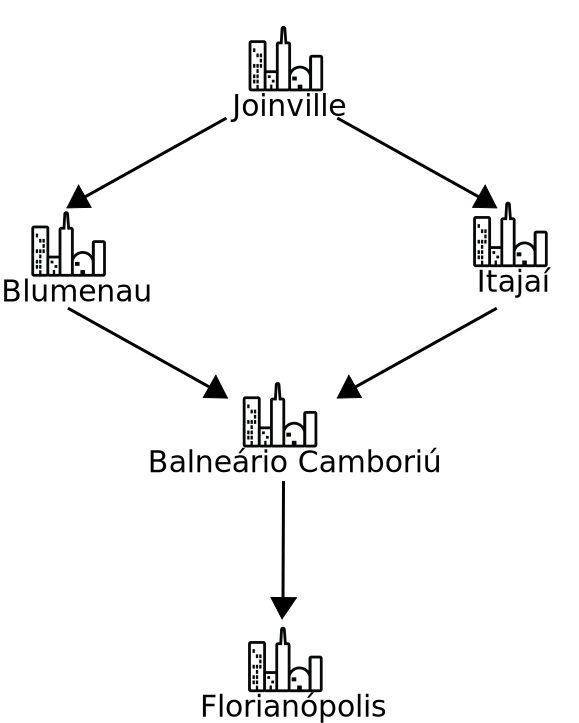
\includegraphics[height=6cm]{cities}
	\end{center}
\end{frame}

\begin{frame}[t]{Inferência em LPO - Passo \#1 = Definir o domínio}	
	$$\begin{array}{lll}
	(1) & estrada(joinville, itajai) & \\
	(2) & estrada(joinville, blumenau) & \\
	(3) & estrada(itajai, balneariocamboriu) & \\
	(4) & estrada(blumenau, balneariocamboriu) & \\
	(5) & estrada(balneariocamboriu, florianopolis) & \\
	\hline
	\end{array}$$	
\end{frame}

\begin{frame}[t]{Inferência em LPO - Passo \#2 = Definir as regras}	
	\begin{tiny}
	$$\begin{array}{lll}
	(1) & estrada(joinville, itajai) & \\
	(2) & estrada(joinville, blumenau) & \\
	(3) & estrada(itajai, balneariocamboriu) & \\
	(4) & estrada(blumenau, balneariocamboriu) & \\
	(5) & estrada(balneariocamboriu, florianopolis) & \\
	(6) & \forall Origem ~\exists Destino: estrada(Origem, Destino) \rightarrow caminho(Origem, Destino) & \\
	(7) & \forall Origem ~\exists Destino: estrada(Origem, Escala) \wedge caminho(Escala, Destino) \rightarrow caminho(Origem, Destino) & \\
	\hline
	\end{array}$$	
	\end{tiny}
\end{frame}

\begin{frame}[t]{Inferência em LPO - Passo \#3 = Definição da Hipótese}	
	\begin{tiny}
	$$\begin{array}{lll}
	(1) & estrada(joinville, itajai) & \\
	(2) & estrada(joinville, blumenau) & \\
	(3) & estrada(itajai, balneariocamboriu) & \\
	(4) & estrada(blumenau, balneariocamboriu) & \\
	(5) & estrada(balneariocamboriu, florianopolis) & \\
	(6) & \forall Origem ~\exists Destino: estrada(Origem, Destino) \rightarrow caminho(Origem, Destino) & \\
	(7) & \forall Origem ~\exists Destino: estrada(Origem, Escala) \wedge caminho(Escala, Destino) \rightarrow caminho(Origem, Destino) & \\
	\hline
	\end{array}$$	
	\end{tiny}

	$$\vdash caminho(joinville, florianopolis)$$
\end{frame}

\begin{frame}[t]{Inferência em LPO - Passo \#4 = Inferência}	
	\begin{tiny}
	$$\begin{array}{lll}
	(1) & estrada(joinville, itajai) & \\
	(2) & estrada(joinville, blumenau) & \\
	(3) & estrada(itajai, balneariocamboriu) & \\
	(4) & estrada(blumenau, balneariocamboriu) & \\
	(5) & estrada(balneariocamboriu, florianopolis) & \\
	(6) & \forall Origem ~\exists Destino: estrada(Origem, Destino) \rightarrow caminho(Origem, Destino) & \\
	(7) & \forall Origem ~\exists Destino: estrada(Origem, Escala) \wedge caminho(Escala, Destino) & \\
	& \rightarrow caminho(Origem, Destino) & \\
	\hline
	(8) & estrada(joinville, itajai) \wedge caminho(itajai, florianopolis) \rightarrow caminho(joinville, florianopolis) & \mathbf{(7)~por~(PU)~\begin{array}{l} Origem/joinville \\ Escala/itajai \\ Destino/florianopolis \end{array}}
	\end{array}$$	
	\end{tiny}

	$$\vdash caminho(joinville, florianopolis)$$
\end{frame}

\begin{frame}[t]{Inferência em LPO - Passo \#4 = Inferência}	
	\begin{tiny}
	$$\begin{array}{lll}
	(1) & estrada(joinville, itajai) & \\
	(2) & estrada(joinville, blumenau) & \\
	(3) & estrada(itajai, balneariocamboriu) & \\
	(4) & estrada(blumenau, balneariocamboriu) & \\
	(5) & estrada(balneariocamboriu, florianopolis) & \\
	(6) & \forall Origem ~\exists Destino: estrada(Origem, Destino) \rightarrow caminho(Origem, Destino) & \\
	(7) & \forall Origem ~\exists Destino: estrada(Origem, Escala) \wedge caminho(Escala, Destino) & \\
	& \rightarrow caminho(Origem, Destino) & \\
	\hline
	(8) & estrada(joinville, itajai) \wedge caminho(itajai, florianopolis) \rightarrow caminho(joinville, florianopolis) & \mathbf{(7)~por~(PU)~\begin{array}{l} Origem/joinville \\ Escala/itajai \\ Destino/florianopolis \end{array}} \\
	(9) & estrada(itajai, balneariocamboriu) \wedge caminho(balneariocamboriu, florianopolis) & \\
	 &  \rightarrow caminho(itajai, florianopolis) &  \mathbf{(7)~por~(PU)~\begin{array}{l} Origem/itajai\\ Escala/balneariocamboriu \\ Destino/florianopolis \end{array}} \\
	\end{array}$$	
	\end{tiny}

	$$\vdash caminho(joinville, florianopolis)$$
\end{frame}

\begin{frame}[t]{Inferência em LPO - Passo \#4 = Inferência}	
	\begin{tiny}
	$$\begin{array}{lll}
	(1) & estrada(joinville, itajai) & \\
	(2) & estrada(joinville, blumenau) & \\
	(3) & estrada(itajai, balneariocamboriu) & \\
	(4) & estrada(blumenau, balneariocamboriu) & \\
	(5) & estrada(balneariocamboriu, florianopolis) & \\
	(6) & \forall Origem ~\exists Destino: estrada(Origem, Destino) \rightarrow caminho(Origem, Destino) & \\
	(7) & \forall Origem ~\exists Destino: estrada(Origem, Escala) \wedge caminho(Escala, Destino) & \\
	& \rightarrow caminho(Origem, Destino) & \\
	\hline
	(8) & estrada(joinville, itajai) \wedge caminho(itajai, florianopolis) \rightarrow caminho(joinville, florianopolis) & \mathbf{(7)~por~(PU)~\begin{array}{l} Origem/joinville \\ Escala/itajai \\ Destino/florianopolis \end{array}} \\
	(9) & estrada(itajai, balneariocamboriu) \wedge caminho(balneariocamboriu, florianopolis) & \\
	 &  \rightarrow caminho(itajai, florianopolis) &  \mathbf{(7)~por~(PU)~\begin{array}{l} Origem/itajai\\ Escala/balneariocamboriu \\ Destino/florianopolis \end{array}} \\
	(10) & estrada(balneariocamboriu, florianopolis) \rightarrow caminho(balneariocamboriu, florianopolis) & \mathbf{(6)~por~(PU)~\begin{array}{l} Origem/balneariocamboriu \\ Destino/florianopolis \end{array}} \\
	\end{array}$$	
	\end{tiny}

	$$\vdash caminho(joinville, florianopolis)$$
\end{frame}

\begin{frame}[t]{Inferência em LPO - Passo \#4 = Inferência}	
	\begin{tiny}
	$$\begin{array}{lll}
	(1) & estrada(joinville, itajai) & \\
	(2) & estrada(joinville, blumenau) & \\
	(3) & estrada(itajai, balneariocamboriu) & \\
	(4) & estrada(blumenau, balneariocamboriu) & \\
	(5) & estrada(balneariocamboriu, florianopolis) & \\
	(6) & \forall Origem ~\exists Destino: estrada(Origem, Destino) \rightarrow caminho(Origem, Destino) & \\
	(7) & \forall Origem ~\exists Destino: estrada(Origem, Escala) \wedge caminho(Escala, Destino) & \\
	& \rightarrow caminho(Origem, Destino) & \\
	\hline
	(8) & estrada(joinville, itajai) \wedge caminho(itajai, florianopolis) \rightarrow caminho(joinville, florianopolis) & \mathbf{(7)~por~(PU)~\begin{array}{l} Origem/joinville \\ Escala/itajai \\ Destino/florianopolis \end{array}} \\
	(9) & estrada(itajai, balneariocamboriu) \wedge caminho(balneariocamboriu, florianopolis) & \\
	 &  \rightarrow caminho(itajai, florianopolis) &  \mathbf{(7)~por~(PU)~\begin{array}{l} Origem/itajai\\ Escala/balneariocamboriu \\ Destino/florianopolis \end{array}} \\
	(10) & estrada(balneariocamboriu, florianopolis) \rightarrow caminho(balneariocamboriu, florianopolis) & \mathbf{(6)~por~(PU)~\begin{array}{l} Origem/balneariocamboriu \\ Destino/florianopolis \end{array}} \\
	(11) & caminho(balneariocamboriu, florianopolis) & \mathbf{(5,10) ~por~(MP)} \\
	\end{array}$$	
	\end{tiny}

	$$\vdash caminho(joinville, florianopolis)$$
\end{frame}

\begin{frame}[t]{Inferência em LPO - Passo \#4 = Inferência}	
	\begin{tiny}
	$$\begin{array}{lll}
	(1) & estrada(joinville, itajai) & \\
	(2) & estrada(joinville, blumenau) & \\
	(3) & estrada(itajai, balneariocamboriu) & \\
	(4) & estrada(blumenau, balneariocamboriu) & \\
	(5) & estrada(balneariocamboriu, florianopolis) & \\
	(6) & \forall Origem ~\exists Destino: estrada(Origem, Destino) \rightarrow caminho(Origem, Destino) & \\
	(7) & \forall Origem ~\exists Destino: estrada(Origem, Escala) \wedge caminho(Escala, Destino) & \\
	& \rightarrow caminho(Origem, Destino) & \\
	\hline
	(8) & estrada(joinville, itajai) \wedge caminho(itajai, florianopolis) \rightarrow caminho(joinville, florianopolis) & \mathbf{(7)~por~(PU)~\begin{array}{l} Origem/joinville \\ Escala/itajai \\ Destino/florianopolis \end{array}} \\
	(9) & estrada(itajai, balneariocamboriu) \wedge caminho(balneariocamboriu, florianopolis) & \\
	 &  \rightarrow caminho(itajai, florianopolis) &  \mathbf{(7)~por~(PU)~\begin{array}{l} Origem/itajai\\ Escala/balneariocamboriu \\ Destino/florianopolis \end{array}} \\
	(10) & estrada(balneariocamboriu, florianopolis) \rightarrow caminho(balneariocamboriu, florianopolis) & \mathbf{(6)~por~(PU)~\begin{array}{l} Origem/balneariocamboriu \\ Destino/florianopolis \end{array}} \\
	(11) & caminho(balneariocamboriu, florianopolis) & \mathbf{(5,10) ~por~(MP)} \\
	(12) & estrada(itajai, balneariocamboriu) \wedge caminho(balneariocamboriu, florianopolis) & \mathbf{(3, 11)~por~(CONJ)} \\
	\end{array}$$	
	\end{tiny}

	$$\vdash caminho(joinville, florianopolis)$$
\end{frame}

\begin{frame}[t]{Inferência em LPO - Passo \#4 = Inferência}	
	\begin{tiny}
	$$\begin{array}{lll}
	(1) & estrada(joinville, itajai) & \\
	(2) & estrada(joinville, blumenau) & \\
	(3) & estrada(itajai, balneariocamboriu) & \\
	(4) & estrada(blumenau, balneariocamboriu) & \\
	(5) & estrada(balneariocamboriu, florianopolis) & \\
	(6) & \forall Origem ~\exists Destino: estrada(Origem, Destino) \rightarrow caminho(Origem, Destino) & \\
	(7) & \forall Origem ~\exists Destino: estrada(Origem, Escala) \wedge caminho(Escala, Destino) & \\
	& \rightarrow caminho(Origem, Destino) & \\
	\hline
	(8) & estrada(joinville, itajai) \wedge caminho(itajai, florianopolis) \rightarrow caminho(joinville, florianopolis) & \mathbf{(7)~por~(PU)~\begin{array}{l} Origem/joinville \\ Escala/itajai \\ Destino/florianopolis \end{array}} \\
	(9) & estrada(itajai, balneariocamboriu) \wedge caminho(balneariocamboriu, florianopolis) & \\
	 &  \rightarrow caminho(itajai, florianopolis) &  \mathbf{(7)~por~(PU)~\begin{array}{l} Origem/itajai\\ Escala/balneariocamboriu \\ Destino/florianopolis \end{array}} \\
	(10) & estrada(balneariocamboriu, florianopolis) \rightarrow caminho(balneariocamboriu, florianopolis) & \mathbf{(6)~por~(PU)~\begin{array}{l} Origem/balneariocamboriu \\ Destino/florianopolis \end{array}} \\
	(11) & caminho(balneariocamboriu, florianopolis) & \mathbf{(5,10) ~por~(MP)} \\
	(12) & estrada(itajai, balneariocamboriu) \wedge caminho(balneariocamboriu, florianopolis) & \mathbf{(3, 11)~por~(CONJ)} \\
	(13) & caminho(itajai, florianopolis) & \mathbf{(9, 12) ~por~(MP)} \\
	\end{array}$$	
	\end{tiny}

	$$\vdash caminho(joinville, florianopolis)$$
\end{frame}

\begin{frame}[t]{Inferência em LPO - Passo \#4 = Inferência}	
	\begin{tiny}
	$$\begin{array}{lll}
	(1) & estrada(joinville, itajai) & \\
	(2) & estrada(joinville, blumenau) & \\
	(3) & estrada(itajai, balneariocamboriu) & \\
	(4) & estrada(blumenau, balneariocamboriu) & \\
	(5) & estrada(balneariocamboriu, florianopolis) & \\
	(6) & \forall Origem ~\exists Destino: estrada(Origem, Destino) \rightarrow caminho(Origem, Destino) & \\
	(7) & \forall Origem ~\exists Destino: estrada(Origem, Escala) \wedge caminho(Escala, Destino) & \\
	& \rightarrow caminho(Origem, Destino) & \\
	\hline
	(8) & estrada(joinville, itajai) \wedge caminho(itajai, florianopolis) \rightarrow caminho(joinville, florianopolis) & \mathbf{(7)~por~(PU)~\begin{array}{l} Origem/joinville \\ Escala/itajai \\ Destino/florianopolis \end{array}} \\
	(9) & estrada(itajai, balneariocamboriu) \wedge caminho(balneariocamboriu, florianopolis) & \\
	 &  \rightarrow caminho(itajai, florianopolis) &  \mathbf{(7)~por~(PU)~\begin{array}{l} Origem/itajai\\ Escala/balneariocamboriu \\ Destino/florianopolis \end{array}} \\
	(10) & estrada(balneariocamboriu, florianopolis) \rightarrow caminho(balneariocamboriu, florianopolis) & \mathbf{(6)~por~(PU)~\begin{array}{l} Origem/balneariocamboriu \\ Destino/florianopolis \end{array}} \\
	(11) & caminho(balneariocamboriu, florianopolis) & \mathbf{(5,10) ~por~(MP)} \\
	(12) & estrada(itajai, balneariocamboriu) \wedge caminho(balneariocamboriu, florianopolis) & \mathbf{(3, 11)~por~(CONJ)} \\
	(13) & caminho(itajai, florianopolis) & \mathbf{(9, 12) ~por~(MP)} \\
	(14) & estrada(joinville, itajai) \wedge caminho(itajai, florianopolis) & \mathbf{(1, 13) ~por~(CONJ)} \\
	\end{array}$$	
	\end{tiny}

	$$\vdash caminho(joinville, florianopolis)$$
\end{frame}

\begin{frame}[t]{Inferência em LPO - Passo \#4 = Inferência}	
	\begin{tiny}
	$$\begin{array}{lll}
	(1) & estrada(joinville, itajai) & \\
	(2) & estrada(joinville, blumenau) & \\
	(3) & estrada(itajai, balneariocamboriu) & \\
	(4) & estrada(blumenau, balneariocamboriu) & \\
	(5) & estrada(balneariocamboriu, florianopolis) & \\
	(6) & \forall Origem ~\exists Destino: estrada(Origem, Destino) \rightarrow caminho(Origem, Destino) & \\
	(7) & \forall Origem ~\exists Destino: estrada(Origem, Escala) \wedge caminho(Escala, Destino) & \\
	& \rightarrow caminho(Origem, Destino) & \\
	\hline
	(8) & estrada(joinville, itajai) \wedge caminho(itajai, florianopolis) \rightarrow caminho(joinville, florianopolis) & \mathbf{(7)~por~(PU)~\begin{array}{l} Origem/joinville \\ Escala/itajai \\ Destino/florianopolis \end{array}} \\
	(9) & estrada(itajai, balneariocamboriu) \wedge caminho(balneariocamboriu, florianopolis) & \\
	 &  \rightarrow caminho(itajai, florianopolis) &  \mathbf{(7)~por~(PU)~\begin{array}{l} Origem/itajai\\ Escala/balneariocamboriu \\ Destino/florianopolis \end{array}} \\
	(10) & estrada(balneariocamboriu, florianopolis) \rightarrow caminho(balneariocamboriu, florianopolis) & \mathbf{(6)~por~(PU)~\begin{array}{l} Origem/balneariocamboriu \\ Destino/florianopolis \end{array}} \\
	(11) & caminho(balneariocamboriu, florianopolis) & \mathbf{(5,10) ~por~(MP)} \\
	(12) & estrada(itajai, balneariocamboriu) \wedge caminho(balneariocamboriu, florianopolis) & \mathbf{(3, 11)~por~(CONJ)} \\
	(13) & caminho(itajai, florianopolis) & \mathbf{(9, 12) ~por~(MP)} \\
	(14) & estrada(joinville, itajai) \wedge caminho(itajai, florianopolis) & \mathbf{(1, 13) ~por~(CONJ)} \\
	(15) & caminho(joinville, florianopolis) & \mathbf{(8, 14)~por~(MP)}
	\end{array}$$	
	\end{tiny}

	$$\vdash caminho(joinville, florianopolis)$$
\end{frame}


\begin{frame}[t]{Inferência em LPO - Exercício}	
	Traduzir os conhecimentos abaixo para LPO (fatos ou regras):

	\begin{enumerate}
	\item Marcos era um homem
	\item Todos os homens e mulheres são pessoas
	\item Marcos nasceu em Pompeia
	\item Todos os que nasceram em Pompeia eram romanos
	\item Cesar era um soberano
	\item Todos os romanos eram leais a Cesar ou o odiavam
	\item As pessoas só tentam assassinar soberanos aos quais não são leais
	\item Marcos tentou assassinar Cesar
	\end{enumerate}

	\vskip 0.5cm

	{\bf Prove que:} Marcos odeia Cesar 
\end{frame}


\begin{frame}[t]{Inferência em LPO - Exercício}
	\begin{tiny}	
	$$\begin{array}{lll}
	(1) & homem(marcos) & \\
	(2) & \forall X: ~homem(X) \vee mulher(X) \rightarrow pessoa(X) & \\
	(3) & pompeano(marcos) & \\
	(4) & \forall X: ~pompeano(X) \rightarrow romano(X) & \\
	(5) & soberano(cesar) & \\
	(6) & \forall X:~romano(X) \rightarrow leal\_a(X, cesar) \vee odeia(X, cesar) & \\
	(7) & \forall X~\exists Y:~ pessoa(X) \wedge soberano(Y) \wedge tenta\_assassinar(X,Y) \rightarrow \sim leal\_a(X,Y) & \\
	(8) & tenta\_assassinar(marcos, cesar) & \\
	\hline
	\end{array}$$	
	\end{tiny}

	$$\vdash odeia(marcos, cesar)$$
\end{frame}


\begin{frame}[t]{Inferência em LPO - Exercício}
	\begin{tiny}	
	$$\begin{array}{lll}
	(1) & homem(marcos) & \\
	(2) & \forall X: ~homem(X) \vee mulher(X) \rightarrow pessoa(X) & \\
	(3) & pompeano(marcos) & \\
	(4) & \forall X: ~pompeano(X) \rightarrow romano(X) & \\
	(5) & soberano(cesar) & \\
	(6) & \forall X:~romano(X) \rightarrow leal\_a(X, cesar) \vee odeia(X, cesar) & \\
	(7) & \forall X~\exists Y:~ pessoa(X) \wedge soberano(Y) \wedge tenta\_assassinar(X,Y) \rightarrow \sim leal\_a(X,Y) & \\
	(8) & tenta\_assassinar(marcos, cesar) & \\
	\hline
	(9) & pessoa(marcos) \wedge soberano(cesar) \wedge tenta\_assassinar(marcos, cesar) & \\
	     & \rightarrow\sim leal\_a(marcos, cesar) & \mathbf{(7) ~por~(PU)~\begin{array}{l} X/marcos \\ Y/cesar \end{array}} \\
	(10) & homem(marcos) \vee mulher(marcos) \rightarrow pessoa(marcos) & \mathbf{(2) ~por~(PU) ~~  X/marcos } \\
	(11) & homem(marcos) \vee mulher(marcos)  & \mathbf{(1) ~por~(AD)} \\
	(12) & pessoa(marcos) & \mathbf{(10, 11) ~por~(MP)} \\
	(13) & pessoa(marcos) \wedge soberano(cesar) & \mathbf{(5, 12) ~por~(CONJ)} \\
	(14) & pessoa(marcos) \wedge soberano(cesar) \wedge tenta\_assassinar(marcos, cesar) & \mathbf{(8,13) ~por~(CONJ)} \\
	(15) &\sim leal\_a(marcos, cesar) & \mathbf{(9,14) ~por~(MP)} \\
	(16) & pompeano(marcos) \rightarrow romano(marcos) & \mathbf{(4) ~por~(PU) ~~X/marcos} \\
	(17) & romano(marcos) & \mathbf{(3, 16) ~por~(MP)} \\
	(18) & romano(marcos) \rightarrow leal\_a(marcos, cesar) \vee odeia(marcos, cesar) & \mathbf{(6) ~por~(PU)~~X/marcos} \\
	(19) & leal\_a(marcos, cesar) \vee odeia(marcos, cesar) & \mathbf{(17, 18) ~por~(MP)} \\
	(20) & odeia(marcos, cesar) & \mathbf{(15, 19) ~por~(SD)} 
	\end{array}$$	
	\end{tiny}

	$$\vdash odeia(marcos, cesar)$$
\end{frame}



\begin{frame}[t]{Resumindo os Elementos da Lógica de Predicados}
	\begin{itemize} 
	\itemsep 0.3cm
	\item Há fatos sobre objetos atômicos: $\{a, b, ..., 0, 1, ...,V, F, ...\}$
	\item Os objetos são pertencentes a um dado domínio: ($D$)
%	\item Estes objetos podem constituir uma classe predicativa
	\item Assim,  há {\bf predicados} que  estabelecem relações entre os objetos
	
	\item Estas relações ou predicados operam sobre objetos de domínios: $$D = D_1 \cup D_2 \cup\ldots\cup D_N$$
	\item Há o conceito de interpretação ou validade da fórmula predicativa, dada por: $\Phi (predicado) = \{V, F\}$
  \item Há ainda, os functores ou funções lógicas, os quais são mapeados em $D$

\item Em resumo, adicione o conceito de conjuntos à lógica proposicional, e define-se
uma lógica mais poderosa: a {\bf lógica de primeira-ordem}.

	\end{itemize}
\end{frame}


\begin{frame}[t]{Exercício}

Considere o seguinte conjunto de f\'ormulas: 
%%%{\bf \textcolor{red}{é boa esta questão ... manteria !}}

\vspace{13pt}

\begin{tabular}{ll}
 \hline \hline
1. &  $\forall x\forall y (q(x,y) \wedge r(y) \rightarrow p(y)) $ \\
2. &  $\forall x  (q(x,x) \rightarrow p(x))  $ \\
3. &  $\forall x \exists y ( s(x) \rightarrow q(x,y)) $ \\
4. &  $r(b)$ \\ 
5. &  $s(a)$ \\
6. &  $s(b)$  \\ 
\hline \hline
\end{tabular}

\vspace{13pt}

Utilizando as propriedades da LPO (por exemplo: PU, GU, GE e PE), demonstre: $\sim p(a)$ \textbf{ ou } $p(a)$ e $\sim p(b)$ \textbf{ ou } $p(b)$. O domínio é dado por $D=\{a,b\}$. 


\end{frame}

\section{PROLOG} % Necessário para gerar o \tableofcontents

\begin{frame}[t]
\vskip 3cm
\begin{center}
{\Huge Introdução à Programação em Lógica}
\end{center}
\end{frame}

\begin{frame}[t]{Programação em Lógica}
	\begin{itemize}
	\item Programação Lógica é um paradigma de programação baseado em linguagens {\bf declarativas}

	\item Um programa declarativo rompe com a noção de \underline{sequencialidade} de instruções lógicas; ao invés disso, trabalha com os conceitos de conhecimento declarativo e procedimental
	
	\item Conhecimento {\bf declarativo} é aquele conhecimento que é especificado cujo uso não foi definido
	
	\item Conhecimento {\bf procedimental} são informações de controle sobre o uso do conhecimento declarativo	
	\end{itemize}
\end{frame}

\begin{frame}[t]{Programação Lógica}
	\begin{itemize}
	\item O processo de se programar através desse paradigma é o que se segue:
	\end{itemize}
	\begin{enumerate}
	\item Modelagem do(s) domínio(s)
	\item Modelagem dos fatos conhecidos acerca do problema
	\item Modelagem das regras conhecidas acerca do problema
	\item Consulta à base de conhecimento
	\item Especificação da inferência desejada (predicado)
	\end{enumerate}
	
	Em caso de sucesso, o \underline{motor de inferência} retorna o predicado com suas variáveis {\bf unificadas}
\end{frame}

\begin{frame}[t]{Programação Lógica - Unificação}
	\begin{itemize}
	\item É o processo do PROLOG reconhecer predicados como sendo \underline{similares}
	
	\item A fim de garantir a similiridade entre predicados os seguintes critérios precisam ser satisfeitos:
	\begin{enumerate}
	\item mesmo nome de predicado
	\item mesma quantidade de parâmetros (aridade)
	\item mesmos valores literais na mesma ordem especificada (caso existam)
	\end{enumerate}
	
	\item Exemplos:
	\begin{itemize}
	\item $homem(joao) \Leftrightarrow homem(X) \equiv MATCH$
	\item $predicado(X, Marcos) \Leftrightarrow predicado(Y) \equiv \mbox{NOT MATCH}$
	\end{itemize}
	
	\item No caso da unificação ocorrer com sucesso, o motor de inferência substitui as variáveis presentes pelos seus respectivos valores unificados. 
	
	Exemplo: no primeiro exemplo acima {\bf X/joao}, ou seja, a variável $X$ é substituída pela constante literal $joao$
	\end{itemize}
\end{frame}

\begin{frame}[t]{Programação Lógica - PROLOG}
	\begin{itemize}
	\item A linguagem de programação lógica {\bf PROLOG} é um exemplo de linguagem declarativa
	
	\item Algumas restrições de representação de predicados são impostas pela linguagem:
	\begin{footnotesize}
	\begin{enumerate}
	\item Todas as expressões são sucedidas pelo símbolo ponto {\bf (.)}
	\item Os quantificadores $\forall$ e $\exists$ não são implementados explicitamente. O que significa que precisam ser representados de forma implícita (como conjunções ou disjunções)
	\item Os operadores lógicos possuem simbologia específica. A saber: $$\wedge ~\equiv~ , \hspace{0.3cm} \vee ~\equiv~ ; \hspace{0.3cm} \rightarrow ~\equiv~ :-$$
	\item As regras de implicação lógica podem conter apenas um predicado no seu consequente: $$homem(X) \wedge humano(X) \rightarrow mortal(X)$$ e ainda, são especificados em sua forma recíproca:\\ {\bf consequente $\rightarrow$ antecedente}: {\scriptsize $$mortal(X) :- homem(X),humano(X)$$}
	\end{enumerate}
	\end{footnotesize}
	\end{itemize}
\end{frame}

\begin{frame}[t]{Exemplo de Programação Lógica (I)}
	\begin{itemize}
	\item ``{\em Hoje fui a uma festa e apresentado a três casais. Os maridos tinham esposas e profissões distintas. Após alguns goles, me confundi quem era casado com quem e suas profissões. Apenas lembro de alguns fatos. Então me ajude a descobrir quem são os casais. Eis os fatos que eu me lembro:}''\footnote{Retirado da Revista Coquetel - Problemas de Lógica}
	\begin{enumerate}
	\item O médico é casado com a Maria
	\item Paulo é advogado
	\item Patrícia não é casada com Paulo
	\item Carlos não é médico
	\item Ah! Luis e Lúcia também estavam na festa
	\item Lembro também que alguém era engenheiro
	\end{enumerate}	 
	\end{itemize}
\end{frame}

\begin{frame}[t]{Exemplo de Programação Lógica (II)}
	Modelagem do Problema:
	
	\begin{itemize}
	\item Podemos identificar três domínios:
	\begin{description}
	\item[Homens (H)] Pedro, Carlos, Luis
	\item[Mulheres (M)] Patrícia, Lúcia, Maria
	\item[Profissões (P)] Médico, Engenheiro, Advogado
	\end{description}
	
	\item Queremos identificar tuplas-3 da forma $(H,M,P)$
	
	\item A solução do problema é então uma lista com 3 dessas tuplas: $$(H1, M1, P1), (H2, M2, P2), (H3, M3, P3)$$
	\end{itemize}
\end{frame}

\begin{frame}[t]{Exemplo de Programação Lógica (III)}
	\begin{itemize}
	\item O processo para desenvolvimento e execução de um programa em PROLOG é o seguinte:
	\end{itemize}
	\begin{enumerate}
	\item Editoração do código do programa em um ou mais arquivos texto (usualmente *.pl)
	\item É necessário ter um motor de inferência PROLOG como {\bf SWI-Prolog}\footnote{\url{http://www.swi-prolog.org/}} ou {\bf tkEclipse}
	\item Consulta ao arquivo fonte através do menu {\bf File | Consult}
	\item Em caso de sucesso na consulta, basta digitar no prompt do ambiente ({\bf ?-}) a inferência desejada (não esqueça do ``.'' !)
	\end{enumerate}
\end{frame}

\begin{frame}[t]{Exemplo de Programação Lógica (IV)}
	\begin{center}
	\includegraphics[width=9.5cm]{interface-swi-prolog}
	\end{center}
\end{frame}

\begin{frame}[fragile]{Exemplo de Programação Lógica (V)}
\begin{center}
{\bf exemplo1.pl}
\end{center}

\begin{scriptsize}
\begin{lstlisting}
profissao(medico).
profissao(engenheiro).
profissao(advogado).

mulher(maria).
mulher(lucia).
mulher(patricia).

festa((carlos, M1, P1), (luis, M2, P2), (paulo, M3, P3)) :-
     mulher(M1), mulher(M2), mulher(M3),
     M1\==M2,M1\==M3,M2\==M3,
     profissao(P1), profissao(P2), profissao(P3),
     P1\==P2,P1\==P3,P2\==P3,
     ((P1 == medico,M1 == maria);(P2 == medico, M2 == maria)),
     P3 == advogado,
     M3 \== patricia,
     P1 \== medico.	
\end{lstlisting}
\end{scriptsize}
\end{frame}

\begin{frame}[t]{Inferência PROLOG com Sentenças Abertas}
	\begin{itemize}
	\item O que nós acabamos de fazer foi uma inferência (em uma base de conhecimento) a partir de uma sentença aberta
	\item Ou seja, na prática o que o PROLOG foi construir uma enumeração de todas as possíveis combinações de particularização das variáveis envolvidas (produto cartesiano) e retornou aquela particularização que satisfez ao predicado inferido
	\item Notem que, dependendo do problema podem haver mais de uma particularização que satisfaz o problema. O Prolog irá apenas mostrar inicialmente a primeira destas. Caso se deseje ver outras possíveis respostas, use a tecla ``{\bf ;}'' (no tkEclipse há um botão na interface para isso)
	\item ``{\bf .}'' encerra o processo
	\end{itemize}
\end{frame}

\begin{frame}[t]{Inferência PROLOG com Sentenças Abertas}
	\begin{itemize}
	\item Mas como funciona o processo de determinação da particularização no Prolog ?
	\item Através de uma abordagem recursiva denominada {\bf backtracking} (retrocesso)
	\item Inicialmente, o sistema particulariza cada variável do predicado sendo inferido com a primeira opção disponível na base de conhecimento
	\item Em seguida, para a \underline{última} variável inferida, uma próxima particularização é determinada
	\item Quando não houverem mais particularizações possíveis para a última variável, então o processo é realizado para a penúltima variável de forma análoga (e assim por diante, para as demais variáveis)
	\end{itemize}
\end{frame}

\begin{frame}[fragile]{Inferência PROLOG com Sentenças Abertas}
\begin{center}
{\bf prodcartesiano.pl}
\end{center}

\begin{lstlisting}
a(1).
a(2).
a(3).
b(alfa).
b(beta).
b(gama).
produto(X,Y) :- a(X),b(Y).
\end{lstlisting}
\end{frame}


\begin{frame}[t]{Inferência PROLOG com Sentenças Abertas}
	\begin{itemize}
	\item Ao inferirmos a sentença ``{\bf produto(A,B).}'' obtemos como resultado todas as particularizações para as variáveis $A$ e $B$ que assumem os valores produzidos para as variáveis $X$ e $Y$ respectivamente: {\bf X/A Y/B}
	\item O resultado obtido é:
	\end{itemize}
	$$\begin{array}{l l}A = 1 & B = alfa \\ A = 1 & B = beta \\ A = 1 & B = gama\\ A = 2 & B = alfa \\ A = 2 & B = beta \\ A = 2 & B = gama\\ A = 3 & B = alfa \\ A = 3 & B = beta \\ A = 3 & B = gama \end{array}$$
\end{frame}


\begin{frame}[t]{Inferência PROLOG com Sentenças Abertas}
	\begin{itemize}
	\item Sempre que uma variável é particularizada por algum predicado, ela permanecerá particularizada pelo restante da interpretação ($\Phi$) daquele predicado (variáveis não mudam de valor durante uma interpretação)
	\item Neste caso, predicados que já tenham suas variáveis particularizadas se tornam `fatos' e são interpretadas pelo Prolog como proposições (V ou F)
	\end{itemize}
\end{frame}


\begin{frame}[fragile]{Inferência PROLOG com Sentenças Abertas}
\begin{center}
{\bf prodcartesiano2.pl}
\end{center}

\begin{lstlisting}
a(1).
a(2).
a(3).
b(1).
b(3).
b(5).
c(X,Y) :- a(Y), b(X).
produto(X,Y) :- a(X),b(Y),c(X,Y).
\end{lstlisting}

\begin{center}
Qual a sequência de particularizações para o predicado ``produto(A,B).'' ?
\end{center}
\end{frame}

\begin{frame}[t]{Prolog - Exercício (I)}
	\begin{enumerate}
	\item Traduzir o exercício dos caminhos e estradas visto em aula, para Prolog
	\item Repetir a inferência ``{\bf caminho(joinville, florianopolis).}'' para confirmar se a programação está correta
	\item Inferir outros caminhos (válidos e inválidos)
	\item Acrescentar novas cidades e estradas ao mapa original
	\end{enumerate}
\end{frame}

\begin{frame}[t]{Prolog - Exercício (II)}
	\begin{enumerate}
	\item Traduzir o exercício do soberano visto em aula, para Prolog
	\item Repetir a inferência ``{\bf odeia(marcos, cesar).}'' para confirmar se a programação está correta
	\end{enumerate}
\end{frame}

\begin{frame}[t]{Prolog - Exercício (III)}
	\begin{enumerate}
	\item Construir um programa em PL para descrever relações familiares em uma árvore genealógica
	\item Considere como fatos: homem, mulher, pai, casal
	\item \underline{Sugestão:} use sua própria família como exemplo
	\item Construa regras para descrever os seguintes predicados: irmão, irmã, avô, avó, tio, tia, primo, prima
	\end{enumerate}

	\vskip 0.3cm

	\begin{center}
	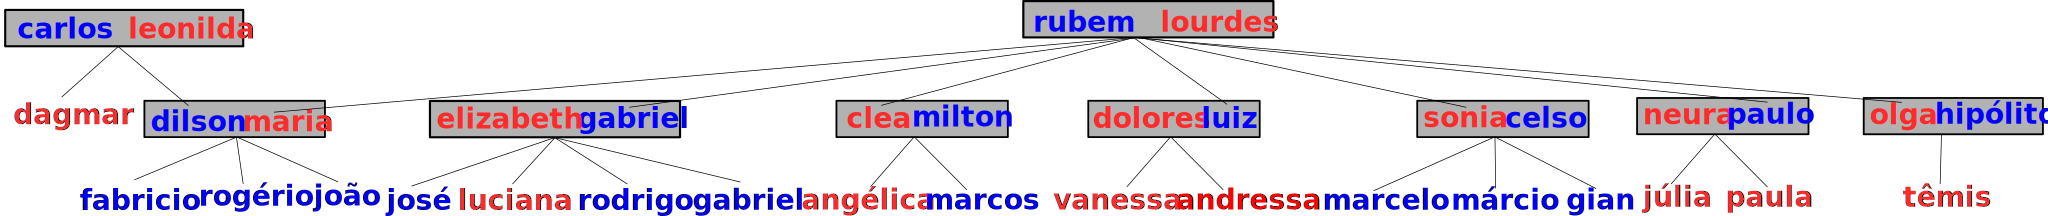
\includegraphics[width=\textwidth]{familia}
	\end{center}
\end{frame}

\begin{frame}[fragile]{Prolog - Exercício (III)}
\begin{center}
{\bf familia-pessoas.pl}
\end{center}

\begin{minipage}{0.4\textwidth}
\begin{tiny}
\begin{lstlisting}
homem(carlos).
homem(rubem).
homem(dilson).
homem(fabricio).
homem(rogerio).
homem(joao).
homem(gabriel).
homem(jose).
homem(rodrigo).
homem(gabrielzinho).
homem(milton).
homem(marcos).
homem(luiz).
homem(celso).
homem(marcelo).
homem(marcio).
homem(gian).
homem(paulo).
homem(hipolito).
\end{lstlisting}
\end{tiny}
\end{minipage}
\begin{minipage}{0.4\textwidth}
\begin{tiny}
\begin{lstlisting}
mulher(leonilda).
mulher(lourdes).
mulher(maria).
mulher(dagmar).
mulher(elizabeth).
mulher(luciana).
mulher(clea).
mulher(angelica).
mulher(dolores).
mulher(vanessa).
mulher(andressa).
mulher(sonia).
mulher(neura).
mulher(julia).
mulher(paula).
mulher(olga).
mulher(temis).
\end{lstlisting}
\end{tiny}
\end{minipage}
\end{frame}

\begin{frame}[fragile]{Prolog - Exercício (III)}
	\begin{center}
	{\bf familia-pais.pl}
	\end{center}

\begin{minipage}{0.4\textwidth}
\begin{tiny}
\begin{lstlisting}
pai(carlos, dilson).
pai(carlos, dagmar).
pai(dilson, fabricio).
pai(dilson, rogerio).
pai(dilson, joao).
pai(rubem, maria).
pai(rubem, gabriel).
pai(rubem, clea).
pai(rubem, luiz).
pai(rubem, sonia).
pai(rubem, paulo).
pai(rubem, olga).
pai(gabriel, jose).
pai(gabriel, luciana).
pai(gabriel, rodrigo).
pai(gabriel, gabrielzinho).
pai(milton, angelica).
pai(milton, marcos).
pai(luiz, vanessa).
pai(luiz, andressa).
pai(celso, marcelo).
pai(celso, marcio).
pai(celso, gian).
pai(paulo, julia).
pai(paulo, paula).
pai(hipolito, temis).
\end{lstlisting}
\end{tiny}
\end{minipage}
\begin{minipage}{0.4\textwidth}
\begin{tiny}
\begin{lstlisting}
casal(carlos, leonilda).
casal(dilson, maria).
casal(rubem, lourdes).
casal(gabriel, elizabeth).
casal(milton, clea).
casal(luiz, dolores).
casal(celso, sonia).
casal(paulo, neura).
casal(hipolito, olga).
\end{lstlisting}
\end{tiny}
\end{minipage}
\end{frame}

\begin{frame}[fragile]{Prolog - Exercício (III)}
	\begin{center}
	{\bf familia-relacoes.pl}
	\end{center}

\begin{minipage}{0.4\textwidth}
\begin{tiny}
\begin{lstlisting}
mae(X,Y) :- mulher(X), pai(W,Y), casal(W,X).
avo(X,Y) :- homem(X), pai(W,Y), pai(X,W).
avo(X,Y) :- homem(X), mae(W,Y), pai(X,W).
avoh(X,Y) :- mulher(X), pai(W,Y), mae(X,W).
avoh(X,Y) :- mulher(X), mae(W,Y), mae(X,W).
irmao(X,Y) :- homem(X), pai(W,X), pai(W,Y), X\==Y.
irma(X,Y) :- mulher(X), pai(W,X), pai(W,Y), X\==Y.
irmaos(X,Y) :- irmao(X,Y) ; irma(X,Y).
tio(X,Y) :- homem(X), pai(W,Y), irmao(X,W) .
tio(X,Y) :- homem(X), mae(W,Y), irmao(X,W).
tio(X,Y) :- homem(X), pai(W,Y), irma(Z,W), casal(X,Z).
tio(X,Y) :- homem(X), mae(W,Y), irma(Z,W), casal(X,Z).
tia(X,Y) :- mulher(X), pai(W,Y), irma(X,W) .
tia(X,Y) :- mulher(X), mae(W,Y), irma(X,W).
tia(X,Y) :- mulher(X), pai(W,Y), irmao(Z,W), casal(Z,X).
tia(X,Y) :- mulher(X), mae(W,Y), irmao(Z,W), casal(Z,X).
primo(X,Y) :- homem(X), pai(W,X), pai(T,Y), irmao(W,T).
primo(X,Y) :- homem(X), pai(W,X), mae(T,Y), irmao(W,T).
primo(X,Y) :- homem(X), mae(W,X), pai(T,Y), irma(W,T).
primo(X,Y) :- homem(X), mae(W,X), mae(T,Y), irma(W,T).
prima(X,Y) :- mulher(X), pai(W,X), pai(T,Y), irmao(W,T).
prima(X,Y) :- mulher(X), pai(W,X), mae(T,Y), irmao(W,T).
prima(X,Y) :- mulher(X), mae(W,X), pai(T,Y), irma(W,T).
prima(X,Y) :- mulher(X), mae(W,X), mae(T,Y), irma(W,T).
\end{lstlisting}
\end{tiny}
\end{minipage}
\end{frame}


\section{Introdução à Lógica Nebulosa} % Necessário para gerar o \tableofcontents

\begin{frame}[t]
\vskip 3cm
\begin{center}
{\Huge Introdução à Lógica Nebulosa}
\end{center}
\end{frame}
\end{document}
